\documentclass[
]{thesis-ekf}
\usepackage[T1]{fontenc}
\PassOptionsToPackage{defaults=hu-min}{magyar.ldf}
\usepackage[magyar]{babel}
\usepackage{mathtools,amssymb,amsthm,pdfpages,float}
\usepackage{xcolor,listingsutf8,caption}
\footnotestyle{rule=fourth}
\newtheorem{tetel}{Tétel}[chapter]
\theoremstyle{definition}
\newtheorem{definicio}[tetel]{Definíció}
\theoremstyle{remark}
\newtheorem{megjegyzes}[tetel]{Megjegyzés}
\definecolor{darkblue}{rgb}{0,0,139}
\definecolor{deepblue}{rgb}{0,0,0.5}
\definecolor{deepred}{rgb}{0.6,0,0}
\definecolor{deepgreen}{rgb}{0,0.5,0}
\renewcommand{\lstlistingname}{kód}
\lstdefinelanguage{TypeScript}{
	keywords={break, case, catch, continue, debugger, default, delete, do, else, finally, for, function, if, in, instanceof, new, return, switch, this, throw, try, typeof, var, void, while, with, class, export, boolean, throw, implements, import, this, public, static, async, await, Requzest, Response, NextFunction, const},
	morecomment=[l]{//},
	morecomment=[s]{/*}{*/},
	morestring=[b]',
	morestring=[b]",
	sensitive=true
}
\lstdefinestyle{python}{
	language=Python,
	inputencoding=utf8,
	basicstyle=\footnotesize\ttfamily,
	tabsize=2,
	numbers=left,
	numberstyle=\tiny\color{gray},
	stepnumber=1,
	numbersep=10pt,
	xleftmargin=2cm,
	xrightmargin=2cm,
	breaklines=true,
	frame=tblr,
	framesep=3pt,
	rulecolor=\color{black!30},
	keywordstyle=\bfseries\color[HTML]{06486A},
	commentstyle=\itshape\color[HTML]{3A7F97},
	stringstyle=\color{deepgreen},
	showstringspaces=false,
	captionpos=b,
	morekeywords={self},
	emph={__init__},
	emphstyle=\ttfamily\color{darkblue}
}
\lstdefinestyle{ts}{
	language=TypeScript,
	inputencoding=utf8,
	basicstyle=\footnotesize\ttfamily,
	tabsize=2,
	numbers=left,
	numberstyle=\tiny\color{gray},
	stepnumber=1,
	numbersep=10pt,
	xleftmargin=2cm,
	xrightmargin=2cm,
	breaklines=true,
	frame=tblr,
	framesep=3pt,
	rulecolor=\color{black!30},
	keywordstyle=\bfseries\color[HTML]{06486A},
	commentstyle=\itshape\color[HTML]{3A7F97},
	stringstyle=\color{deepgreen},
	showstringspaces=false,
	captionpos=b,
	emphstyle=\ttfamily\color{darkblue},
	escapeinside={\%*}{*)}
}
\def\UrlBreaks{\do\/\do-}
\newcommand{\benchmarkSpecification} {Ezt egy \emph{i7-7700HQ} 2.8 Ghz processzorral és egy \emph{16 GB DDR4 SDRAM}-mal ellátott laptopon futtattam.}
\newcommand{\benchmarkSpecificationSec} {Ezt egy \emph{i5-13600K} 3.5 Ghz processzorral és egy \emph{32 GB DDR5 RAM}-mal ellátott asztali számítógépen futtattam.}

\begin{document}
\institute{Matematikai és Informatikai Intézet}
\title{Ajánlórendszerek és azok integrálása webalkalmazásokban}
\author{Besenyei Ferenc\\Programtervező Informatikus BSc}
\supervisor{Dr. Kovásznai Gergely\\Egyetemi docens}
\city{Eger}
\date{2024}
\maketitle
\tableofcontents

\chapter*{Bevezetés}
\addcontentsline{toc}{chapter}{Bevezetés}
Az elmúlt időszakban, nem telik el úgy nap, hogy ne jöjjön velünk szembe valamilyen \emph{mesterséges intelligenciáról} szóló hír, legyen az egy önvezető jármű, nyelvi modell, vagy az első ``AI Software Engineer''. Azonban a ``mesterséges intelligencia'' kifejezés már régóta létezik, kutatják és fejlesztik. Sokkal több felhasználási területe van, mint azt egy átlagember gondolná és sokkal többször is találkozik vele. A technológia fejlődésének hála, ma már ``mindenki'' zsebében ott lapul egy \emph{okostelefon} és elérhető számára az \emph{internet}. Nem is kell az interneten böngésznünk, már a számítógép operációs rendszer telepítése alatt, a telepítő engedélyt kér, hogy adatokat gyűjtsön viselkedésünkről és \emph{személyre szabott} hirdetésekkel bombázhasson. Ugyanígy majd minden weboldal azzal kezd, hogy engedélyünket kéri, \emph{cookie}-k formájában adatokat gyűjthessen rólunk hasonló célokra. De ott vannak a különböző szociális- és videómegosztó oldalak \emph{hírfolyamai}, melyeket minden nap látogatunk, és még sorolhatnám.

A szakdolgozatom célja, hogy egy átfogó képet nyújtsak a \emph{gépi tanulásról} és az ehhez kapcsolódó különböző területekről. Ugyanígy, az \emph{ajánlórendszerek} témakörét is szeretném bővebben kifejteni, azok különböző megközelítéseit, módszereit, és azt, hogy hogyan tudjuk mindezt megvalósítani és integrálni egy modern webalkalmazásban.

\chapter{Felhasznált technológiák ismertetése}
Az alkalmazás -- ami megtalálható a \url{https://github.com/fepu08/szakdolgozat} GitHub tárolóban az \textbf{mvp} mappában -- egy elosztott rendszer, melyet három részre, szolgáltatásra bontok: 
\begin{itemize}
	\item \emph{Frontend szolgáltatás}:  A böngészőben látható weblap. A felhasználó számára ez a kezelőfelület.
	\item \emph{Backend szolgáltatás}: Többek közt a frontendet és az intelligens szolgáltatást köti össze.
	\item \emph{Intelligens szolgáltatás}: Itt készíti az alkalmazás az ajánlásokat.
\end{itemize}
A rendszerek közötti kommunikációt \emph{HTTP} protokollon keresztül valósítom meg. Bővebben majd \aref{subsec-architektura}. fejezetben, először hadd mutassam be az alkalmazáshoz felhasznált különböző technológiákat. 

\section{TypeScript}
A \emph{TypeScript}\footnote{TypeScript hivatalos oldala: \url{https://www.typescriptlang.org/}} egy ingyenes és nyílt forráskódú, a \emph{Microsoft} által fejlesztett magas szintű programozási nyelv, ami statikus típusossággal és opcionális típusannotációkkal egészíti ki a \emph{JavaScript}-et, annak \emph{szuperszettje}, tehát minden \emph{JavaScript} program szintaktikailag érvényes \emph{TypeScript} kód. Egyaránt használható kliens- és szerver oldalon is, többek közt a \emph{Node.js} használatával.\cite{wiki-ts} Fordítási időben képes hibát dobni, ezáltal gyorsabb visszacsatolást biztosít a fejlesztők számára. Valamint \aref{sec-statikus-kodelemzo}. fejezetben említett \emph{ESlint}-tel együtt használva, a fejlesztés alatt, valós időben láthatjuk a hibát a fejlesztőkörnyezetben. Igazából ez ugyanúgy működik, ahogy \emph{VisualStudio} jelzi a hibát, ha egy \emph{integer} változónak egy \emph{stringet} adunk értékül.

\section{Statikus kódelemző}
\label{sec-statikus-kodelemzo}
Statikus kódelemzéshez az \emph{ESLint}\footnote{ESLint hivatalos oldala: \url{https://eslint.org/}}-et használom kliens- és szerver oldalon egyaránt. Jól működik a \emph{TypeScript}-tel és \emph{Prettier}\footnote{Prettier hivatalos oldala: \url{https://prettier.io/}}-rel. Utóbbival együtt használva szép, egységesen formázott kódot kapunk végeredményként.

\section{Kliens oldali technológiák}
A frontendünk egy \emph{egylapos webalkalmazás} (single page application vagy SPA) mely megépítéséhez a \emph{React} könyvtárat használtam.
\subsection{React}
A \emph{React}\footnote{React hivatalos oldala: \url{https://react.dev/}} egy ingyenes és nyílt forráskódú kliensoldali \emph{JavaScript könyvtár}, melyet komponensalapú felhasználói felületek létrehozásához használnak. A \emph{Meta} (korábban \emph{Facebook}), valamint \emph{open-source fejlesztők} által fejlesztett és üzemeltetett.\cite{wiki-react}

Lényegében azért választottam, mert népszerű, és lehetővé teszi a komponensalapú fejlesztést, valamint nem utolsó sorban ezzel van tapasztalatom. \Aref{fig-react-component-based}. ábrán látható, hogy mit is takar a komponensalapú fejlesztés. Az ábra bal felében a \emph{VideoList} nevű komponens programkódja látható, mely böngészőben való megjelenítésé az ábra jobb felén helyezkedik el. Nem mennék bele a részletekbe, viszont számomra nagy előny ebben a koncepcióban, hogy a \emph{React} egységbe zárja a komponenst és az ahhoz tartozó üzleti logikát, emellett ezek a komponensek \emph{újrafelhasználhatóak}.

\begin{figure}[H]
	\centering
	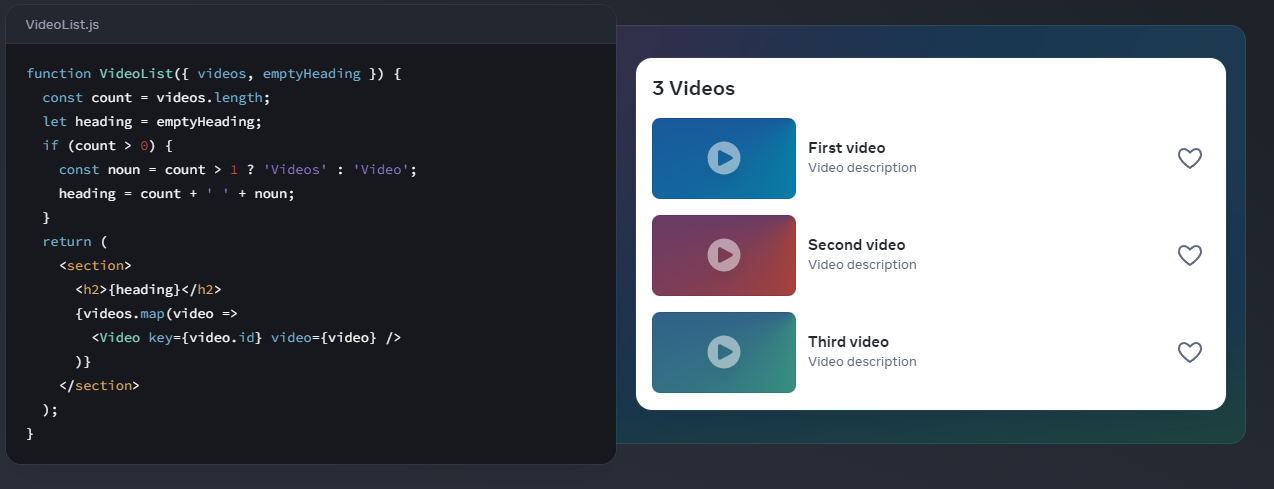
\includegraphics[width=14cm]{images/react-component-based.png}
	\caption[React - Komponensalapú fejlesztés]{React - Komponensalapú fejlesztés\footnotemark}
	\label{fig-react-component-based}
\end{figure}
\footnotetext{Forrás: \url{https://react.dev/}}

\subsection{Egyéb csomagok, könyvtárak, keretrendszerek}
Mivel nem vagyok túl jártas \emph{frontend} fejlesztő, szerettem volna gyorsan és hatékonyan egy szerény, azonban \emph{adaptív}\footnote{A responsive és reactive web design-ról bővebben: \url{https://www.linkedin.com/pulse/reactive-vs-responsive-web-design-complete-comparison-g9fef/}} oldalt létrehozni. Ehhez a \emph{Bootstrap}\footnote{Bootstrap hivatalos oldala: \url{https://getbootstrap.com/}}-et alkalmaztam, ami egy ingyenes és nyílt forrású \emph{CSS keretrendszer}. Továbbá a filmekhez, a borítók gyanánt az \emph{Unsplash} API-át\footnote{Unsplash API - Get a random photo:  \url{https://unsplash.com/documentation\#get-a-random-photo}} használtam. Minden egyéb használt csomag megtalálható a frontend szolgáltatás \emph{package.json} fájljában felsorolva.

\section{Szerver oldali technológiák}
\subsection{Node.js}
A \emph{Node.js}\footnote{Node.js hivatalos oldala: \url{https://nodejs.org/en}} egy aszinkron eseményvezérelt (event-driven) JavaScript futtatókörnyezet, amely skálázható hálózati alkalmazások fejlesztéséhez lett tervezve.\cite{nodejs-homepage}

Noha a \emph{Node.js} nagyon elterjedt és \emph{kiválóan alkalmazható webszerverek, vagy más webes szolgáltatások készítésére}, ugyanakkor megvannak a maga korlátai. Ilyen korlát például az, hogy \emph{egy folyamatban} (process) fut, viszont \emph{nem hoz létre új szálakat minden híváshoz}.\cite{node-docs} Ez annyit jelent a gyakorlatban, hogy ha hosszú, komplikált, nagy számítási kapacitást igénylő műveleteket szeretnék végrehajtani \emph{szinkron} módon, az bizony blokkolja a program futását. Például ha az ajánlórendszer modelljét tanítjuk, vagy a modell segítségével készítünk Top-N ajánlási listát az összes felhasználó számára, azok a felhasználók, akik csak le szeretnék kérni, hogy milyen új filmek vannak, bizony várniuk kell, míg a program végre nem hajtja a műveletet (kész nincs az ajánlási lista), és csak azután tudjuk egyetlen felhasználó kérését fogadni. Ezt orvosolva, a \emph{Node.js}, pontosabban a \emph{libuv} könyvtár\footnote{libuv hivatalos oldala: \url{https://libuv.org/}} létrehozott egy úgynevezett \emph{Event Loop}-ot\footnote{Event Loop: \url{https://nodejs.org/en/learn/asynchronous-work/event-loop-timers-and-nexttick}}, ami egy eseményvezérelt, nem blokkoló I/O modell, mely \emph{lehetővé teszi a Node.js számára hogy egyetlen szálon képes legyen kezelni sok aszinkron műveletet}. Tehát, ha a szerver éppen egy felhasználó kiszolgálásával van elfoglalva, egy másik nyugodtan tud kéréseket intézni a szerverhez, és amint lehetséges válaszolni fog rá.

\subsection{Express}
Az \emph{Express.js}\footnote{Express.js hivatalos oldala: \url{https://expressjs.com/}} vagy Express egy Node.js webalkalmazás-keretrendszer, ami széleskörű funkcionalitást kínál webes és mobilalkalmazások számára.\cite{expressjs-homepage}


Az \emph{Express} a \emph{felelősségi lánc} (chain of responsibility) viselkedési mintát alkalmazva, \emph{köztes szoftverekből} (middleware) áll. A felelősségi lánc viselkedési minta lehetővé teszi, hogy kezelők láncolatán kéréseket továbbítson. A kérés beérkezésekor minden kezelő eldönti, hogy feldolgozza-e a kérést, vagy továbbítja azt a következő kezelőnek a láncban. Minden kezelő képes megállítani a folyamatot, valamint módosítani az objektumot, melyet átadnak egymásnak.\cite{chain-of-responsibility} Ezzel lehetővé válnak különböző funkcionalitások, mint például az autentikáció.

\subsection{Sequelize}
A \emph{Sequelize}\footnote{Sequelize hivatalos oldala: \url{https://sequelize.org/}} egy modern \emph{TypeScript} és \emph{Node.js} \emph{objektum-relációs leképzést megvalósító csomag} (ORM), amit különböző relációs adatbázisokhoz, mint például \emph{PostgreSQL} vagy \emph{MySQL} használhatunk.\cite{sequelize}

Minden egyéb használt csomag megtalálható a backend szolgáltatás \emph{package.json} fájlban felsorolva.

\section{Intelligens rendszerben használt technológiák}
\subsection{Python}
A \emph{Python}\footnote{Python hivatalos oldala: \url{https://www.python.org/}} egy interpretált, magas szintű, multiparadigmás (többek közt funkcionális és objektum-orientált) programozási nyelv, dinamikus szemantikával.

Népszerű és széles körben alkalmazzák az \emph{adattudomány} (data science), \emph{mesterséges intelligencia} (artificial intelligence vagy AI) és a gépi tanulás (machine learning vagy ML) területein is. Ezáltal rengeteg használható eszköz áll rendelkezésünkre, úgy mint a \emph{Surprise} könyvtár, \emph{pandas} vagy a \emph{numpy}. Kiválóan lehet vele szkripteket írni, ahogy az például \aref{subsec-adatbazis-terv}. fejezetben is olvasható. Valamint a \emph{Flask}-hoz hasonló könyvtárakkal \emph{API}-okat is lehet velük létrehozni.

\subsection{Flask}
A \emph{Flask}\footnote{Flask hivatalos oldala: \url{https://flask.palletsprojects.com/en/3.0.x/}} egy \emph{Python}-hoz készült \emph{micro könyvtár}\cite{wiki-flask}, mely segítségével könnyen és egyszerűen tudunk létrehozni egy \emph{REST API}-t, hogy az elkészített ajánlások elérhetők legyenek a backend részére.

\subsection{Surprise könyvtár}
\label{subsec-surpriselib}
A \emph{Surprise}\footnote{Surprise hivatalos oldala: \url{https://surpriselib.com/}} könyvtár egy Python \emph{scikit}, mellyel  explicit értékeléseket használva ajánlórendszereket tudunk építeni és analizálni.\cite{surpriselib}

Megtalálhatók benne előre implementált csomagok (package) és modulok (module), úgy mint: 
\begin{itemize}
	\item \emph{prediction\_algorithms package}: Különböző előrejelző algoritmusok ajánlások készítéséhez.
	\item \emph{model\_selection package}: Különböző keresztvalidációhoz és hiperparaméter-\\finomhangoláshoz szükséges eszközök.
	\item \emph{similarities module}: Elemek közötti hasonlóság kiszámítására szolgáló algoritmusok.
	\item \emph{accuracy module}: Pontossági mérőszámok kiszámításához funkciók.
	\item \emph{dataset module}: Adatkészletek menedzseléséhez.
	\item \emph{dump module}: Betanított modellek és elkészült ajánlások szerializálásához, mentéséhez, betöltéséhez.
\end{itemize}\cite{surpriselib}

Minden egyéb használt csomagot megtalálni az intelligens szolgáltatás \emph{requirements.txt} fájljában, köztük a \emph{pandas} és \emph{numpy} csomagokat.

\section{Adatbázis-kezelő rendszer}
Az \emph{adatbázis} elektronikusan tárolt és elérhető adatok szervezett gyűjteménye. Az \emph{adatbázis-kezelő rendszer} (Database Management System vagy DBMS) az a szoftver, amely az adatok rögzítése és elemzése érdekében kapcsolatban áll a végfelhasználókkal, az alkalmazásokkal és magával az adatbázissal. A DBMS-szoftver emellett magában foglalja az adatbázis kezeléséhez biztosított alapvető eszközöket is. Számos népszerű \emph{DBMS} létezik, melyeket különböző típusokra lehet osztani az alapján, hogy milyen formában tárolják az adatokat.\cite{wiki-adatbazis}

\subsection{PostgreSQL}
\label{subsec-postgres}
Az alkalmazáshoz \emph{PostgreSQL}\footnote{PostgreSQL hivatalos oldala: \url{https://www.postgresql.org/}} (vagy Postgres) választottam. A Postgres egy ingyenes, nyílt forráskódú \emph{relációs adatbázis-kezelő rendszer} (RDMS), amit sokan kedvelnek számos előnye miatt, például támogatja az SQL nyelvet és olyan adattípusokat mint \emph{JSON}, jól skálázható a particionálásnak köszönhetően, biztonságos, stb.\cite{postgres-docs}

\section{Docker}
A \emph{Docker}\footnote{Docker hivatalos oldala: \url{https://www.docker.com/}} egy szoftver platform, melyet alkalmazások fejlesztésére, futtatására és szállítására fejlesztettek. A Docker segítségével elkülöníthető az applikációnk és az infrastruktúra, lehetővé téve a gyorsabb fejlesztés.\cite{docker-overview} Operációs rendszer szintű virtualizációt, úgynevezett konténerizációt hajt végre. A hagyományos virtualizációtóval ellentétben, a Docker egyetlen operációs rendszer kernelt használ az összes konténer számára, így jelentős mértékben csökkentve a szükséges erőforrásokat és növelve a hatékonyságot. Docker \emph{konténerek} futtatására szolgál, melyek egymástól elszeparált, zárt környezetek. Ezek képesek más konténerekkel és a külvilággal kommunikálni. Az egyes konténerek létrehozásához \emph{képfájlokat} (imagefile vagy image) használ, ezek a konténert leíró fájlok, tartalmaznak mindent, ami egy szoftver futtatásához szükséges, beleértve a programkódot, futtatókörnyezetet, könyvtárakat, környezeti változókat és konfigurációs fájlokat. A konténerek segítségével képesek vagyunk automatizálni az applikációk telepítését és futtatását, így azok zökkenőmentesen tudnak különböző környezetekben, izoláltan működni.\cite{docker-docs, docker-overview-container, docker-overview-image}

\subsection{Docker Compose}
A \emph{Docker Compose} egy eszköz, mely leírja és futtatja a több konténerből álló alkalmazásokat. Leegyszerűsíti az alkalmazás irányítását, segítségével könnyen lehet szolgáltatásokat, hálózatot és köteteket (volume)\footnote{Docker volumes:  lehetővé teszi az adatok tárolását és azok konténerek közötti megosztását.} menedzselni egy egyszerű, átfogó \emph{YAML}\footnote{A YAML egy elterjedt, emberek által könnyen olvasható, szerializációs nyelv, melyeket gyakran használnak konfigurációs fájlokban. Forrás: \url{https://en.wikipedia.org/wiki/YAML}} fájlban.\cite{docker-compose-docs}
\chapter{Gépi Tanulás}
\section{Mi az a Gépi Tanulás?}

	A gépi tanulás (Machine Learning) kifejezést 1959-ben \emph{Arthur Samuel}, az IBM egyik alkalmazottja alkotta meg. A gépi tanulásra úgy is hivatkoztak, hogy \emph{öntanító} vagy \emph{önoktató számítógépek} (``self-teaching computers'').\cite{wiki-ml}

	A gépi tanulás a számítógép-tudomány és \emph{mesterséges intelligencia} (MI, angolul artificial intelligence vagy AI) egy ága, ami lehetővé teszi a számítógépek olyan dolgok elvégzésére, melyre nem programozták őket -- nem adtak utasításokat, nem definiálták előre a lépéseket. Ezt nem úgy kell érteni, hogy a gépek programozás nélkül teljesítenek feladatokat, sokkal inkább úgy, hogy a beviteli adatokat (input data), nem pedig a beviteli parancsokat (input command) használva hajtják azt végre.\cite{book:ml-for-beginners}
	
	Fontos észben tartani, ahogy az \aref{fig-mestint-reszhalmazai}. ábrán is látható, a gépi tanulás nem ekvivalens a mesterséges intelligenciával, hanem csak egy részhalmaza annak. Míg a \emph{gépi tanulás} olyan algoritmusokat jelent, melyek képesek az említett tanulásra, előrejelzéseket és döntéseket elvégezni a beviteli adat alapján, addig a \emph{mesterséges intelligencia} alatt a program vagy mesterségesen létrehozott tudat által megnyilvánuló intelligenciát értjük.\cite{wiki-aihun, wiki-aieng} \emph{Alan Turing} volt az első, aki jelentős kutatásokat végzett a mesterséges intelligencia területén, amit \emph{gépi intelligenciának} (machine intelligence) nevezett.\cite{wiki-aihun, wiki-aieng}
	
	\begin{figure}[H]
		\centering
		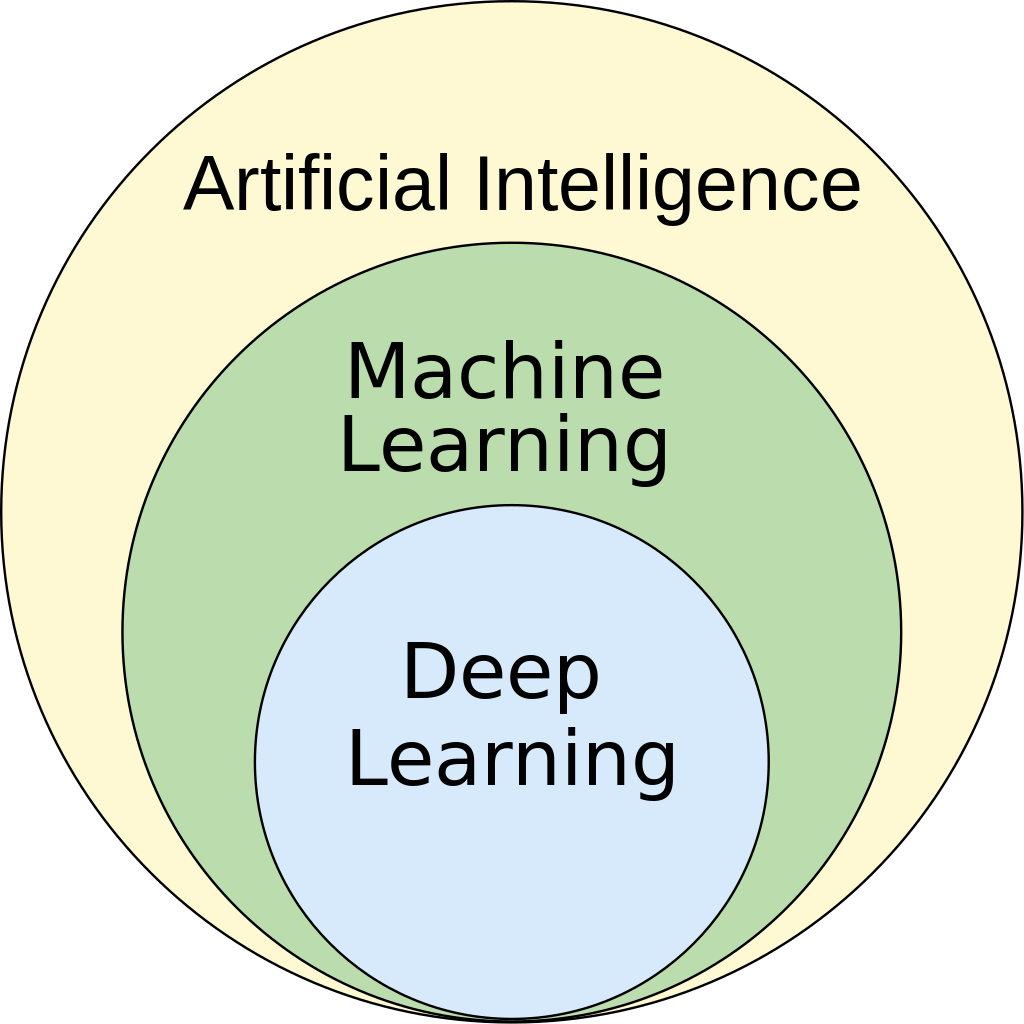
\includegraphics[width=6cm]{images/ml-subfield-of-ai.png}
		\caption[A mesterséges intelligencia részhalmazai]{A mesterséges intelligencia részhalmazai\footnotemark}
		\label{fig-mestint-reszhalmazai}
	\end{figure}
	\footnotetext{Forrás: \cite{bioinformatics-in-ml}}
	
	A gépi tanulást megannyi területen használják, mint például: 
	\begin{itemize}
		\item csalások feltárása (fraud detection)
		\item levélszemét szűrők (spam)
		\item beszéd felismerés (speech recognition)
		\item természetes nyelvek feldolgozása (natural language processing vagy NLP)
		\item gépi látás (computer vision)
		\item egészségügy
		\item önvezető járművek
		\item \emph{ajánló rendszerek} (recommender systems) melyet a szakdolgozatom témájának választottam, bővebben \aref{chap-ajanlo-rendszerek}. fejezetben olvashatunk róla.
	\end{itemize}

\section{A gépi tanulás lépései}
\label{gepi-tanulas-lepesei}
	\Acite{ml-lifecycle} felhasználva a gépi tanulást a következő lépésekre lehet bontani:
	\begin{enumerate}
		\item \textbf{A probléma definiálása}: Mit szeretnénk megoldani?
		\item \textbf{Adatgyűjtés}: Az algoritmusunk tanításához.
		\item \textbf{Adatok előkészítése, előfeldolgozása}: Például a hiányzó értékek kezelése, normalizálás.
		\item \textbf{Az adatok elemzése}: Annak érdekében, hogy megértsük a mintákat, trendeket és összefüggéseket. Ezek segítenek a feladatokhoz szükséges jellemzőkészletek definiálásában (feature engineering).
		\item \textbf{Jellemzők definiálása} (Feature engineering): ``A feature engineering az adatbányászat első fázisa, amelyikben az adatokat gyűjtjük össze, egészen pontosan az általunk fontosnak tartott “jellemzőket” (features).''\cite{featureengineeringmagyaritas}
		\item \textbf{Algoritmus kiválasztása}: Az eddig végzett lépések alapján a megfelelő ML algoritmus kiválasztása. Fontos szempontok pl. a probléma, amit meg szeretnénk oldani és az adat természete.
		\item \textbf{Az adat elosztása}: A gépi tanuláshoz a teljes adathalmazt általában két vagy három diszjunkt részre bontjuk, lásd \aref{az-adat-keszletekre-valo-felosztasa}. fejezetben.
		\item \textbf{A modell tanítása}: ``A tanító adatbázis alapján, a kiértékelési metrika, mint célfüggvényre optimalizálva, a gépi tanulás során felépítunk egy modellt. A modell a döntési szabály, ami tartalmazza az egyedek jellemzői közti feltárt kapcsolatokat\allowbreak/mintázatokat\allowbreak/szabályszerűségeket.''\cite{gepitanulasalapfogalmak}
		\item \textbf{A modell kiértékelése}: Különböző metrikákkal (bővebben \aref{sec-algoritmusok-kiertekelese}. fejezetben) (például RMSE) a tesztkészletet felhasználva.
		\item \textbf{Hiperparaméter-finomhangolás} (Hyperparameter Tuning): A modell paramétereinek finomhangolása a jobb eredmény eléréséhez
		\item \textbf{Üzembe helyezés}
		\item \textbf{Felhasználói visszacsatolás} (Feedback Loop): A rendszer javításának, fejlesztésének érdekében.
	\end{enumerate}
	
\section{Adat}
\label{sec-adat}
	Ahogy az előző pontban is látható, a beviteli adat, amivel majd a modell tanítva lesz, nagyban befolyásolja az algoritmus kimenetét. A több mennyiségű adat nem feltétlenül jelent azt, hogy jobban teljesít majd a betanított modell. Nagyon fontos, hogy az adatot megfelelően előkészítsük a feldolgozásra. Kulcsfontosságú, hogy lehetőleg csak a releváns adatokat tartsuk meg, ugyanakkor, ahogy a későbbiekben olvasható, előfordulhat, hogy a modell új, számunkra ismeretlen összefüggéseket fedez fel (lásd \aref{subsec-unsupervised-learning}. fejezet). Megeshet, hogy az adatban sok jellemző hiányos (missing data), vagy nulla értékű (sparse data).
	
	\begin{itemize}\label{sparse-data}
		\item \textbf{Ritka adat}: olyan adatkészletekre utal, ahol sok bejegyzés értéke 0 vagy egy alapértelmezett nem informatív érték (például null).
		\item \textbf{Hiányos adat}: olyan adathiányra utal, mely valamilyen hiba miatt, az adatok váratlanul nem állnak rendelkezésünkre.
	\end{itemize}
	
	\begin{figure}[!h]
		\centering
		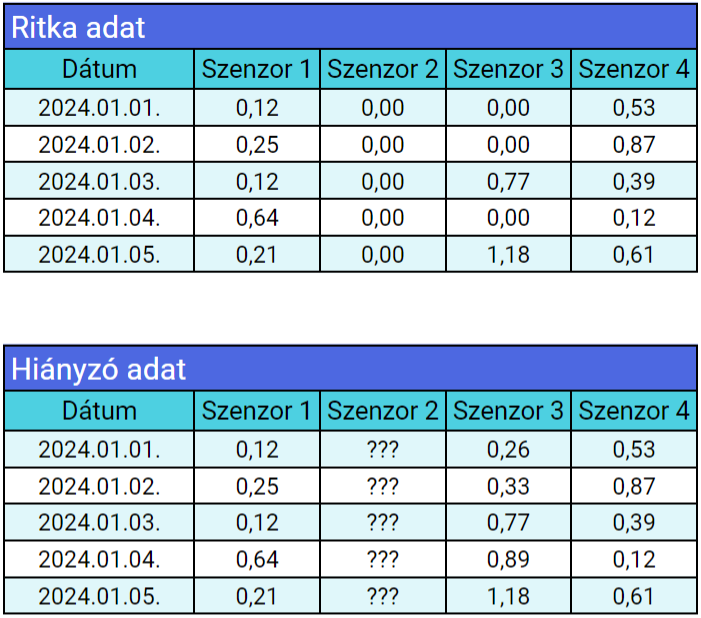
\includegraphics[width=8cm]{images/ritka-es-hianyzo-adat.png}
		\caption[Ritka és hiányzó adatok reprezentálása]{Ritka és hiányzó adatok reprezentálása\footnotemark}
		\label{ritka-es-hianyzo-adat}
	\end{figure}
	\footnotetext{Forrás: \url{	https://stats.stackexchange.com/questions/267322/difference-between-missing-data-and-sparse-data-in-machine-learning-algorithms}}	

	
	\Aref{ritka-es-hianyzo-adat} ábrán látható, hogy míg a \emph{ritka adat} az a \emph{Szenzor 2-nél} és sok helyen a \emph{Szenzor 3-nál} 0 értékű -- tehát a mérések és az adat küldések megtörténtek -- addig a \emph{hiányzó adat} táblában a \emph{Szenzor 2} valamiért nem küldött mérési adatokat. Ugyanakkor gépi tanulás kontextusában mindkettőre gyakran csak ``sparse data''-ként hivatkoznak. Vannak olyan módszerek, algoritmusok, melyek nem működnek jól ilyen adatokkal (például memória-alapú kollaboratív szűrők, lásd \aref{subsec-kollaborativ}. fejezetben), de vannak, amelyeket ilyen esetekre használnak (például \emph{SVD}, lásd \aref{subsec-dimenzio-csokkentes}. fejezet).
	
	Az adatok sok forrásból jöhetnek, \emph{különböző formákban}. Ilyen szempontból megkülönböztethetünk:
		\begin{itemize}
			\item \textbf{Struktúrált adat}: Adatbázis táblák.
			\item \textbf{Strukturálatlan adat}: Szöveg, kép, hang, videó, stb.
			\item \textbf{Félig Strukturált (Semi-Structured) adat}.
		\end{itemize}
		
	Valamint az \emph{adat mennyisége} is eltérő lehet:
	\begin{itemize}
		\item \textbf{Data}: Általában strukturált formában van tárolva, pár terrabájt nagyságrendig.
		\item \textbf{Big Data}: Strukturálatlan vagy félig strukturált formában van tárolva, pár terrabájttól egészen több exabájt ($1EB \approx 10^6TB$) nagyságrendig.
	\end{itemize}
	Ezek persze több dologban is eltérhetnek, ugyanakkor érdemesnek tartottam megemlíteni ezeket a szempontokat.
	
	A \emph{táblázatos adat} (tabular-data) olyan adatkészlet, amely táblákban, sorokba és oszlopokba van rendezve.\cite{tabular-data-def} Az oszlopok a \emph{jellemzőket}  (variable, dimension, attribute, feature) és a sorok reprezentálják az \emph{egyedeket} (példány, instance, row, case, value), egy adott jellemzőn való megfigyeléseket (lásd \ref{fig-tabular-data}.~ábra).\cite{book:ml-for-beginners,gepitanulasalapfogalmak}
	
	\begin{figure}[!h]
		\centering
		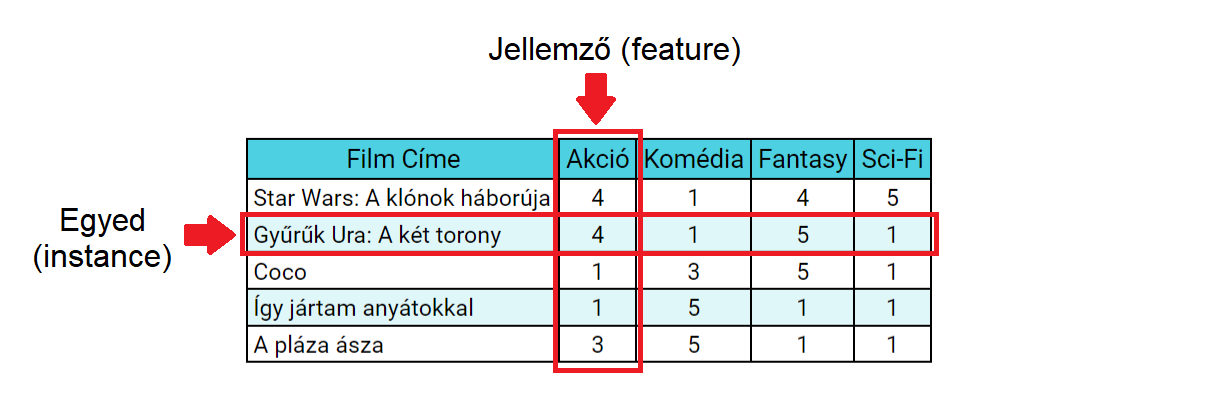
\includegraphics[width=14cm]{images/tabular-data.PNG}
		\caption{Táblázatos adat\cite{gepitanulasalapfogalmak}}
		\label{fig-tabular-data}
	\end{figure}
	
	Az oszlopokat lehet \emph{vektoroknak} is nevezni és több vektorra lehet \emph{mátrixként} is hivatkozni (lásd \ref{fig-vektor-matrix}.~ábra). A felügyelt tanulásnál, a sorok már léteznek az adatkészletben és arra használjuk őket, hogy a mintázatokat fedezzünk fel az egymástól független jellemzők közt.\cite{book:ml-for-beginners}
	\begin{figure}[!h]
		\centering
		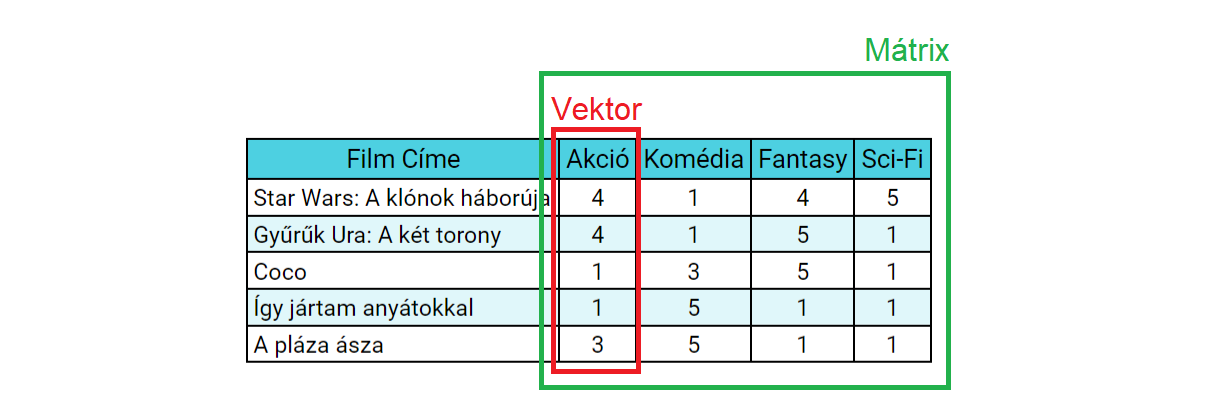
\includegraphics[width=14cm]{images/vektor-matrix.png}
		\caption{Vektor és Mátrix táblázatos adatnál\cite{book:ml-for-beginners}}
		\label{fig-vektor-matrix}
	\end{figure}
	
	
\subsection{Az adat tisztítása}
Az adat változatossága miatt -- például hiányzó, ritka, vagy éppen strukturálatlan adat -- az adatot elő kell készíteni mielőtt a modellt elkezdjük rajta tanítani. Ezt a lépést angolul ``Data Scrubbing''-nak nevezik.

A tisztítás alatt több dologra is oda kell figyelnünk, úgy mint:
\begin{itemize}
	\item Duplikációk
	\item Szenzitív információk törlése vagy anonimizálása
	\item Ritka, vagy hiányos adat
	\item Az adat standardizálása
	\item Normalizáció
\end{itemize}

\subsection{Az adat gyűjtése}
Az adat gyűjtése történhet \emph{explicit} és \emph{implicit} módon.

Az explicit adatgyűjtés általában a rendszer által, a felhasználótól kért adatbevitelt jelent, például:
\begin{itemize}
	\item Adjon értékelést
	\item Válassza ki a listából az általa legjobban preferált cikkeket
\end{itemize}

Mivel a felhasználók nagy többsége valamely oknál fogva nem szeret explicit értékelést adni, ezért sokszor az implicit adatgyűjtés jelenti a megoldást. Ez a módszer számos előnnyel rendelkezik, többek közt lehetővé teszi sokkal szélesebb körű és változatosabb adatok gyűjtését:

\begin{itemize}
	\item a felhasználó mikor és mivel lépett interakcióba (például megtekintett egy árucikket)
	\item egy filmet, videót vagy terméket mennyi ideig nézett
	\item mit és mivel vásárolt együtt
\end{itemize}

\subsection{Az adat készletekre való felosztása}
\label{az-adat-keszletekre-valo-felosztasa}
A gépi tanuláshoz az a teljes adathalmazt általában három diszjunkt részre bontjuk:
\begin{itemize}
	\item \textbf{Tanító készlet} (train set): A rendelkezésre álló adat nagy részét -- az összes adat 60-80\%-át -- a modell tanítására, azaz a modell paramétereinek a beállítására használjuk fel.
	
	\item \textbf{Validációs készlet} (validation set): Ezt az adathalmazt a \emph{hiperparaméterek finomhangolására} (lásd \ref{sec-hiperparameter-optimalizalas}. fejezet), valamint \emph{regularizációra} (az \emph{idő előtti leállítás} segítségével) használjuk, amellyel elkerülhető a túlilleszkedés. Az összes adat 10-20\%-át kitevő részhalmaz.
	
	\item \textbf{Tesztelési készlet} (test set): A tesztelési (esetleg tesztelő vagy teszt) készlet egy a modell számára új, ismeretlen adathalmaz. Ezt használjuk a modell teljesítményének mérésére (lásd \ref{sec-algoritmusok-kiertekelese}. fejezet). Az összes adat 10-20\%-a.

\end{itemize}\cite{introduction-to-statistical-learning}

Ugyanakkor előfordul, hogy az adatot csak \emph{tanító és tesztelő készletekre} bontják. Például akkor, ha nincs elegendő adatmennyiség vagy számítási kapacitás, vagy -- ahogy a szakdolgozatomban is -- amikor \emph{keresztvalidációt} (lásd \ref{subsec-cross-validation}. fejezet) használnak, mely lehetővé teszi az adat hatékonyabb felosztását.

\section{Tanulási típusok}
\subsection{Felügyelt tanulás}
A felügyelt tanulás (supervised learning) során a gépet \emph{címkézett} (labeled) adatkészletekkel tanítják, hogy felismerje az adatok közötti mintákat és mintázatokat, majd megtanulja a bemutatott példákat megfelelően címkézni. Mivel a tanítási adatokat már előre ellátták a helyes címkékkel, a modell visszajelzést kap a döntéseinek pontosságáról. Ennek köszönhetően a betanított modell képes lesz arra is, hogy olyan új adatokat is címkékkel ellásson, amelyekkel korábban még nem találkozott.\cite{supervised-learning-google, gepi-tanulas-3-fo-tipusa}

A felügyelt tanulást két fő kategóriába soroljuk: \textbf{klasszifikációs} (vagy osztályozó) és \textbf{regressziós} algoritmusokra. A klasszifikációs feladatok során gyakran alkalmazott módszer a \emph{Logisztikus regresszió}, míg a regressziós problémák megoldására gyakran használják a \emph{Lineáris regressziót}.\cite{wiki-ml, supervised-learning-google}

\subsection{Felügyelet nélküli tanulás}
\label{subsec-unsupervised-learning}
A felügyelet nélküli tanulásnál (unsupervised learning vagy self-learning) az emberek által nem ellenőrzött, címkézetlen adatokat szolgáltatnak bemenetként. Mivel ezeket az adatokat nem látták el címkékkel, így a gépnek lehetősége van arra, hogy saját maga fedezze fel az adatok közötti összefüggéseket és kapcsolatokat.\cite{unsupervised-learning-google}

A felügyelet nélküli tanulás különösen jól működik nagyobb komplexitású feladatok esetében, mint például nagy adatkészletek klaszterezésénél -- \emph{``A klaszteranalízis egy olyan dimenziócsökkentő eljárás, amellyel adattömböket tudunk homogén csoportokba sorolni, klasszifikálni.''}\cite{wiki-klaszteranalízis}.

\subsection{Félig felügyelt tanulás}
A félig felügyelt tanulásnál (semi-supervised learning) az adatok diverzitása, strukturálatlansága és nagy volumene, valamint az emberi kapacitás korlátozottsága miatt az adatok többsége nem rendelkezik címkékkel. Azonban, egy kis mennyiségű címkézett adat felhasználásával jelentősen javítható a tanulási folyamat sebessége és pontossága. Ezzel együtt járó hátránya, hogy a rendszer a címkézett adatok esetleges hibáit is megtanulhatja.\cite{semi-supervised-learning-mit,mi-a-gepi-tanulas}

\subsection{Megerősítéses tanulás}
A \emph{megerősítéses tanulás} (reinforcement learning) a modelleket úgy tanítja döntések hozatalára, hogy az optimálishoz közeli végeredményt érjék el. A megerősítéses tanulási algoritmusok a \emph{jutalmazási és büntetési mechanizmusokra épülnek}, és a kapott visszajelzésből vonnak le következtetéseket, annak érdekében, hogy saját maguk fedezzék fel a cél elérésének optimális módját. Képesek a késleltetett jutalmazás alkalmazására is, ami lehetővé teszi számukra, hogy hosszú távon a legjobb eredményeket érjék el, még akkor is, ha ez rövid távon nem tűnik a legkifizetődőbbnek.\cite{what-is-reinforcement-learning}

A való életben ez nagyban hasonlít ahhoz, ahogy az emberek, vagy például a kutyák tanulnak. Vegyük azt az esetet, amikor egy kutyát arra tanítunk, hogy az ``ül'' parancsra leüljön. Jutalomfalatokat használhatunk, és amikor a kutyának mondjuk a parancsszót és ő leül, kap egy falatot; ha viszont nem tesz eleget a parancsnak, akkor nem jutalmazzuk. Így a kutya idővel megtanulja a parancsszót és a hozzá tartozó cselekvést, valamint azt, hogy hogyan szerezheti meg a lehető leggyorsabban a kívánt jutalmat.

\section{Hiperparaméter optimalizálás}
\label{sec-ml-hiperparameter-optimalizalas}
\emph{Hiperparaméterek} azok a konfigurációs beállítások, amelyek meghatározzák a gépi tanulási modellek működését, de nem keverendők össze sem az adathalmaz adatelemeivel, sem a modellek belső paramétereivel, mint például a súlyok vagy a bias. 

Ezek a paraméterek, mint például a neurális hálózatokban a \emph{rétegek száma}, a \emph{tanulási sebesség}, vagy az \emph{aktivációs funkciók}, nem a tanulási folyamat során, hanem előzetesen, manuális beállítással vagy automatizált keresési módszerekkel kerülnek optimális értékre állításra. 

A hiperparaméter-finomhangolás, amelyet az angol szakirodalom ``Hyperparameter-Tuning'' vagy ``Hyperparameter-Optimization'' néven ismer, elengedhetetlen a modell hatékonyságának maximális kiaknázása szempontjából. Ennek ellenére ez a feladat gyakran jelentős kihívást jelent a számos lehetséges konfigurációs kombináció miatt.
Az optimális hiperparaméter-kombinációk megtalálásának több módja létezik, de a legegyszerűbbek közé tartozik a \emph{rácskeresés} (grid search) -- melyet az alkalmazásban használok, és \aref{sec-hiperparameter-optimalizalas}. fejezetben be is mutatom -- vagy a \emph{paraméter-söprés} (parameter sweep), amely egy kimerítő keresési technika a hiperparaméter-tér kézzel meghatározott részhalmazán. Ezt a keresési módszert valamilyen teljesítménymutatóval kell vezérelni, mint például a keresztvalidáció (cross-validation) (lásd \aref{subsec-cross-validation}. fejezet).\cite{aws-hyperparameter-tuning,wiki-hyperparameter-optimization}

\chapter{Ajánló rendszerek}
\label{chap-ajanlo-rendszerek}
Az \emph{ajánló rendszerek} (recommender-, recommendation system, engine vagy algorithm) speciális \emph{információ szűrű rendszerek}, amelyek felhasználói és termékprofilokat építenek tanuló algoritmusok segítségével, majd a modellek alapján ajánlanak olyan \emph{tartalmakat} (film, zene, videó, stb.) vagy \emph{termékeket} a felhasználónak, amely nagy valószínűséggel érdekes lesz számára.\cite{wiki-ajánlórendszer-marketing,wiki-recommender-system,werner-ajanlo-rendszer}

\section {Mely problémákra nyújtanak megoldást?}
Az internet növekedése, az online tartalom mennyisége miatt a felhasználók számára nehézzé vált az információ szűrése, a releváns tartalmak megtalálása, ez az \emph{információs túlterhelés}.\cite{werner-ajanlo-rendszer}

Ugyanakkor, üzleti szempontból is megvannak a nehézségei  az online térben való érvényesülésnek, hiszen a konkurenciák száma is nőttön nő, akiknek a kínálata is sokkal széleskörűbb lehet. Így, hogy minél több és minél elégedettebb felhasználó legyen -- és természetesen minél többet fogyasszanak -- az üzleteknek érdekük segíteni a felhasználót, hogy könnyen megtalálják a számukra megfelelő termékeket, esetleg olyan termékeket is megvásároljanak, amit amúgy nem állt szándékukban, viszont látják, hogy mások, a termék mellé, mely más termékeket vásárolták (Lásd \ref{fig-amazon-frequently-bought-together}~ábra alján a ``Frequently bought together'' részt).

Ahogy azt olvashatjuk \aref{sec-kulonbozo-megkozelitesek}~részben, erre és ehhez hasonló problémákra különböző megközelítéseket hoztak létre.

\begin{figure}[H]
	\centering
	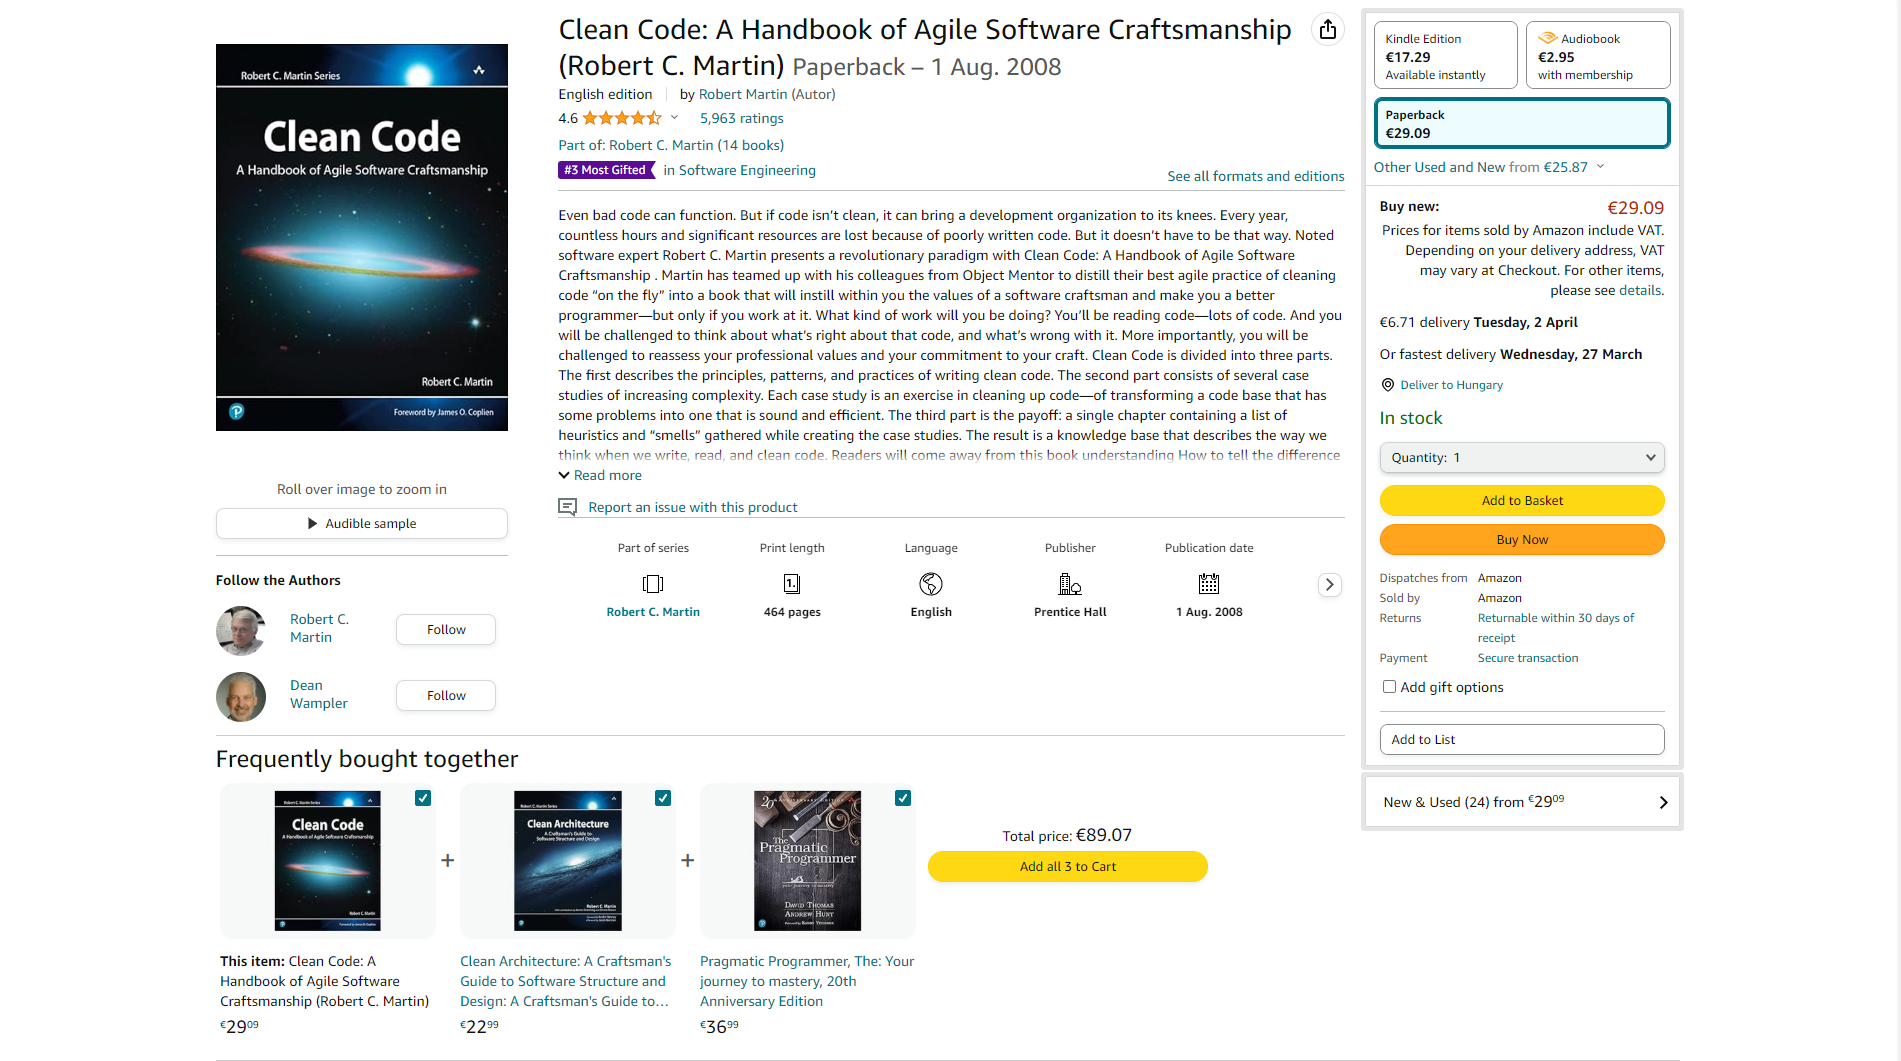
\includegraphics[width=14cm]{images/amazon-frequently-bought-together.png}
	\caption[Példa a gyakran együtt vásárolt termékekre]{Példa a gyakran együtt vásárolt termékekre\footnotemark}
	\label{fig-amazon-frequently-bought-together}
\end{figure}
\footnotetext{Forrás: \url{https://amazon.de}}

\section{Ajánlási feladat formális leírása}
\label{sec-ajanlasi-feladat-formalis-leirasa}
Ebben az alfejezetben az ajánlási feladat formális leírásához a \cite{werner-ajanlo-rendszer} munkájában leírtakat használom.
\subsection{Hasznosságfüggvény}
Ha $C$ jelöli a felhasználókat és $S$ a termékeket, akkor 
\[u\colon C\times S\rightarrow \mathbb{R} , \text{ ahol } \mathbb{R} \text{ halmaz teljesen rendezett,}\]
jelöli a \emph{hasznosságfüggvényt}.\cite{werner-ajanlo-rendszer}
\subsection{Tanulási feladat}
Határozzuk meg azt az ${u}'\colon C\times S\rightarrow \mathbb{R}$ leképzést, amely a lehető legjobban közelíti $u$-t és teljesen definiált a teljes $C\times S$ téren.\cite{werner-ajanlo-rendszer}
\subsection{Ajánló rendszer kimenete}
``$\forall c\in C$ vásárló számára a legérdekesebb/leghasznosabb új termék(ek) megadása, azaz:
\[s_{c}\in S \text{ ,ahol } u(c,s_{c}) \text{ maximális.}\]
''\cite{werner-ajanlo-rendszer}

\section{Hasonlósági függvények}
\label{sec-hasonlosagi-fuggvenyek}
Ahogy azt a későbbiekben is olvashatjuk, az ajánlórendszerek számára szükséges, hogy meg tudjuk határozni a felhasználók vagy az elemek közötti \emph{hasonlóságot}. Erre a célra különböző módszerek állnak a rendelkezésünkre, például: 
\begin{itemize}
	\item \textbf{Euklideszi norma} (Euclidean distance): Két pont közé eső szakasz hosszának meghatározására szolgál.\cite{wiki-tavolsag}
	\[\sqrt{\sum^{n}_{i=1}|x_{i}-y_{i}|^{2}}\]
	
	\item \textbf{Pearson-féle korrelációs együttható} (Pearson correlation coefficient):``olyan mérőszám, amely az erősségét és az irányát mutatja meg egy lineáris kapcsolat két változója között, amely a változók kovarianciája osztva a standard szórás. Ez a korrelációs együttható legismertebb és leggyakrabban használt típusa."\cite{wiki-korrelacios-egyutthato}
		
	\item \textbf{Spearman rangkorrelációs együttható} (Spearman's rank correlation coefficient):``azt jelzi, hogy a két változó közötti kapcsolatot hogyan lehet monoton függvénnyel leírni.''\cite{wiki-korrelacios-egyutthato}
	
	\item \textbf{Jaccard-hasonlóság} (Jaccard similarity): A halmazok közötti hasonlóságot úgy méri, hogy a halmazok metszetének méretét elosztja a halmazok uniójának méretével. Különösen hasznos azoknál a rendszereknél, ahol az adatok binárisak, például megtekintette/nem tekintette meg.\cite{book:introduction-to-data-minging}

\end{itemize}
\subsection{Koszinusz hasonlósági függvény}
\label{koszinusz-hasonlosagi-fuggveny}
A \emph{koszinusz hasonlóság} (cosine similarity) a dokumentumok hasonlóságának egyik legelterjedtebb mértéke, mely két nem nulla vektor hasonlóságának megállapítására szolgál. A koszinusz hasonlóságnál, ahogy a nevéből is következtethető, a \emph{vektorok által bezárt szög koszinusza}, vagyis a vektorok \emph{skaláris szorzata}\footnote{Skaláris szorzatról bővebben: \cite{wiki-skalaris-szorzat}} osztva a hosszuk szorzatával.\cite{book:introduction-to-data-minging, wiki-cosine-similarity}

\begin{definicio}
	\label{def:cosine-similarity}
	Két nem nulla vektor koszinusza az \emph{Euklideszi skalárszorzat} képletének segítségével számítható, ahol $x$ és $y$ két nem nulla vektor, és az általuk bezárt $\theta$ szög koszinusza meghatározható:
	\[ cos(\theta) =\frac{x\cdot y}{\left \|  x \right \| \left \|  y \right \|} \]\label{math-expr:cosine-similarity}
	
	Ahol $x \cdot y$ az $x$ és $y$ vektorok közötti \emph{skaláris szorzatot}, $n$ pedig a dimenziók számát jelöli:
	\[x\cdot y=\sum^{n}_{i=1}x_{i}y_{i}=x_{1}y_{1}+x_{2}y_{2}+\dots +x_{n}y_{n}\]
	
	
	$\left \|  x \right \|$ és $\left \| y \right \|$ pedig $x$ és $y$ vektorok hosszát, vagy Euklideszi normáját jelenti:
	\[\left \| x \right \|= \sqrt{\sum^{n}_{i=1}x^{2}_{i}}=\sqrt{x^{2}_{1}+x^{2}_{2} \dots x^{2}_{n}}\]
	és 
	\[\left \| y \right \|= \sqrt{\sum^{n}_{i=1}y^{2}_{i}}=\sqrt{y^{2}_{1}+y^{2}_{2} \dots y^{2}_{n}}\]
	
\cite{book:introduction-to-data-minging, wiki-skalaris-szorzat, wiki-euklideszi-norma}
\subsubsection{Példa}
Vegyük például a \emph{Free Guy (2021)} akció/vígjáték és a klasszikus \emph{Drágán add az életed! (1988)} akció/thriller filmeket. Az egyszerűség kedvéért, nézzük csak az akció és a vígjáték műfajokat. Képzeljünk el egy koordináta rendszert, ahol az $x$ az \emph{akció} az $y$ tengely pedig a \emph{vígjáték} jellemzőt reprezentálja egy 0-1 skálán. Ha ezen elhelyezzük a \emph{Drágán add az életed!}  filmet az a $[1,0]$ míg a \emph{Free Guy} az $[1,1]$ pontokon helyezkednek el. Ha az origóból húzunk egy-egy vektort ezekbe a pontokba, megkaphatjuk az általuk bezárt $\theta$ szöget, és így kiszámíthajuk a köztük lévő hasonlóságot a \emph{koszinusz hasonlósági} függvényt használva.
\end{definicio}

\subsubsection{Többdimenziós terek}
Az előző példában ugyan az egyszerűség kedvéért két dimenzióban szemléltettem a koszinusz hasonlósági függvényt, ugyanakkor ettől több is lehet. Az applikációban használt adatkészletben számszerűen 19 darab műfaj található. A fenti definíció azonban ugyanúgy alkalmazható 19 dimenziós vektorokra, mint 2 dimenziósokra.


\section{Különböző megközelítések}
\label{sec-kulonbozo-megkozelitesek}
Az ajánló rendszerek algoritmusainak különféle megközelítése ismert:
\begin{itemize}
	\item Kollaboratív szűrők (lásd \aref{subsec-kollaborativ}.~fejezetben)
	\item Tartalomalapú módszerek (content-based filtering): a felhasználó által kedvelt jellemzőkkel bíró termékek (lásd \aref{subsec-tartalomalapu}. fejezet)
	\item Mátrix faktorizáció (lásd \aref{subsec-matrix-faktorizacio})
	\item Mély tanulás (deep learning)
	\item Faktorizáló gépek (factorization machines)
	\item Munkamenet-alapú ajánlások (session-based recommendations)
	\item Gráf-alapú ajánlások (graph based recommendations)
	\item Hibrid modellek (hybrid models): A különböző megközelítéseket kombinálva, azok előnyeit egyesítve, hátrányaikat ellensúlyozza.
\end{itemize}

\subsection{Kollaboratív szűrés}
\label{subsec-kollaborativ}
A \emph{kollaboratív szűrés} (collaborative filtering) \emph{múltbéli} felhasználói interakciók és preferenciák, implicit vagy explicit értékelések alapján ajánl új, még nem értékelt termékeket. Azt a feltételezést veszi alapjául, hogy ha az embereknek megegyezett az ízlése a múltban (például többen is ugyan azokat a filmeket kedvelték, vagy éppen ellenkezőleg) akkor a jövőben is egyetértésre jutnak.\cite{wiki-recommender-system,werner-ajanlo-rendszer,wiki-collaborative-filtering}
	
\begin{figure}[!h]
	\centering
	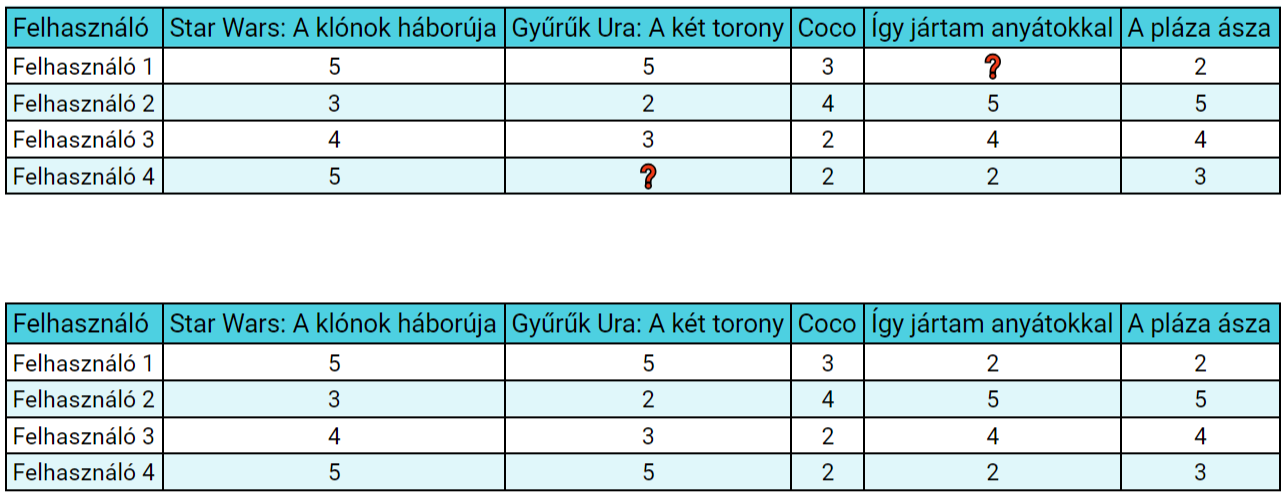
\includegraphics[width=14cm]{images/collaborative-filtering.PNG}
	\caption{Kollaboratív szűrés reprezentálása}
	\label{fig-collaborative-filtering}
\end{figure}

Ahogy \aref{fig-collaborative-filtering}.~ábrán, a felső táblázat mutatja, a \emph{Felhasználó 1} és a \emph{Felhasználó 4} sor hiányos elemekkel rendelkeznek. Mivel a \emph{Felhasználó 1} kedveli a \emph{Star Wars-t} és a \emph{Gyűrűk Urát}, viszont a \emph{Pláza ászát} nem, ezért logikusnak tűnik, hogy a sci-fi és a fantasy műfajokat szereti, a komédiát viszont nem. Párhuzam vonható közte és a \emph{Felhasználó 4} preferenciái közt, ezért következtethetjük, hogy a \emph{Felhasználó 4}-nek tetszeni fog a \emph{Gyűrűk Ura}, míg a \emph{Felhasználó 1}-et nem fogja érdekelni az \emph{Így jártam anyátokkal}. Nagyjából ez a gondolatmenet alkalmazható a gépi tanulás, különösen a kollaboratív szűrési algoritmusok területén is. Azonban fontos figyelembe venni, hogy nem felhasználó párokról beszélünk, hanem hasonló ízléssel bíró felhasználók által adott értékelések (legyenek azok implicit vagy explicit értékelések) aggregálásáról.

A \cite{wiki-recommender-system,werner-ajanlo-rendszer,wiki-collaborative-filtering} források szerint, a kollaboratív szűrési módszereket két osztályra lehet bontani, a \emph{memória alapú} (memory-based) és a \emph{modell alapú} (model-based) megközelítésekre. A \emph{memória alapú} megközelítések közvetlenül az adatbázisban lévő felhasználó-elem interakciókat használják fel az ajánlások előállításához, míg a \emph{modell alapú} megközelítések \emph{előrejelző modelleket} építenek a felhasználói preferenciák és az elemek közötti kapcsolatok modellezésére.

\subsubsection{Memória alapú megközelítések}
A \emph{memória alapú megközelítés} további csoportokra osztható:
\begin{itemize}
	\item \textbf{Felhasználó alapú szűrés} (user-based filtering): Felhasználók közötti hasonlóság alapján tesz ajánlásokat (lásd a fentebb lévő példát és \aref{fig-collaborative-filtering} ábrát). Általában az alábbi két lépésre bontható az algoritmus:
	\begin{enumerate}
		\item Az aktuális felhasználóval (aki számára készíti az ajánlást) hasonló ízlésű felhasználókat keres az értékelési minták vizsgálatával
		\item A hasonló ízlésű felhasználók értékeléseit felhasználva becslést készít az aktuális felhasználó számára
	\end{enumerate}\cite{wiki-collaborative-filtering}
	\item \textbf{Elem alapú szűrés} (item-based filtering): Az elemek közötti hasonlóság alapján tesz ajánlásokat, például ha sok felhasználó szeret egy könyvet, és azok közül sokan szeretnek egy másikat, akkor annak, aki kedveli az egyiket, ajánljuk a másikat (lásd \aref{fig-amazon-frequently-bought-together} ábra alját). Általában az alábbi két lépésre bontható az algoritmus:
	\begin{enumerate}
		\item Épít egy elem-elem mátrixot amely meghatározza az elempárok közötti kapcsolatot
		\item A mátrix vizsgálatával és a felhasználó adatainak egyeztetésével következtet az aktuális felhasználó ízlésére.
	\end{enumerate}\cite{wiki-collaborative-filtering}
	\item \textbf{Hibrid} (hybrid): A felhasználó és elem alapú módszerek előnyeit kombinálja. \cite{hybrid-user-item-based-collaborative-filtering}
\end{itemize}

A felhasználó- és az elem-alapú szűrésekre gyakran hivatkoznak \emph{szomszéd-alapú} kollaboratív szűrőként (neighborhood-based collaborative filtering) is.

Különböző algoritmusokat használnak a hasonlóságok mérésére, például \emph{k-legközelebbi szomszéd} (k-nearest neighbor, röviden k-NN) és a \emph{Pearson korreláció} (Pearson Correlation) (lásd \ref{sec-hasonlosagi-fuggvenyek}. fejezet).\cite{wiki-recommender-system, wiki-collaborative-filtering}

\subsubsection{Modell alapú megközelítések}
\label{subsubsec-kollaborativ-modell-alapu-megkozelitesek}
A \emph{modell alapú} megközelítésekre példa:
\begin{itemize}
	\item \textbf{Bayes-hálók} (Bayesian networks): A csomópontok a termékek, és lehetséges állapotaik az egyes  értékelések.\cite{werner-ajanlo-rendszer} Ezek a hálózatok a valószínűségi következtetések és döntéshozatali folyamatok modellezésére szolgálnak.
	\item \textbf{Klaszterezésen alapuló módszerek} (clustering models): A hasonló ízlésű felhasználókat egy-egy osztályba soroljuk, lehetővé téve az ajánlások személyre szabását a felhasználók klaszterei alapján.\cite{werner-ajanlo-rendszer}
	\item \label{kollaborativ-szures-matrix-faktorizació} \textbf{Mátrix faktorizáció} (matrix factorization): A felhasználó-elem interakció mátrixot két kisebb dimenziójú  mátrix szorzatára bontják (lásd \aref{fig-matrix-factorization}. ábra). Ilyen módszer például az \emph{SVD} (szinguláris érték dekompozíció vagy angolul singular value decomposition) amit az applikációban is implementáltam, bővebben később, \aref{subsec-matrix-faktorizacio}.~fejezetben.
	\item \textbf{Neurális hálózatokon alapuló megközelítések} (neural network-based): Az adatokból mély tanulási modellek segítségével történő mintázatfelismerés és ajánlás, ami képes a bonyolultabb felhasználói interakciók és preferenciák modellezésére.\cite{journal-neural-collaborative-filtering}
\end{itemize}\cite{wiki-collaborative-filtering}

\begin{figure}[!h]
	\centering
	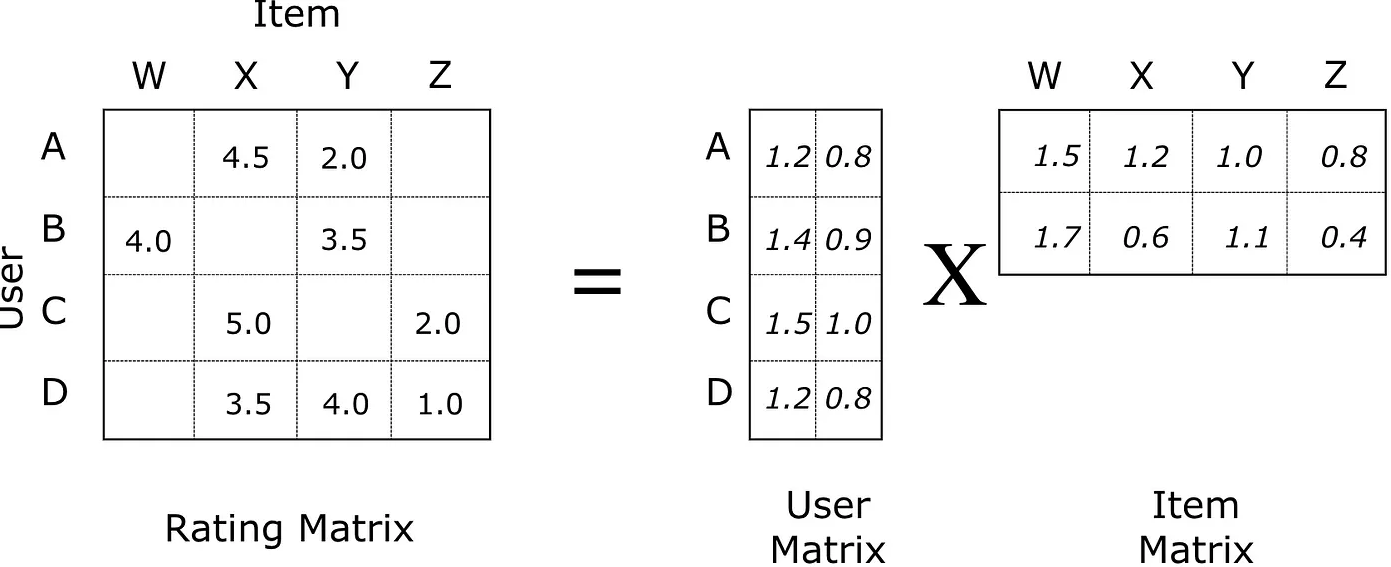
\includegraphics[width=12cm]{images/matrix-factorization.png}
	\caption[Mátrix faktorizáció film értékelés táblán]{Mátrix faktorizáció film értékelés táblán\footnotemark}
	\label{fig-matrix-factorization}
\end{figure}
\footnotetext{Forrás: \cite{prototyping-a-recommender-system-step-by-step-part-2}}

\subsubsection{Előnyei}
A kollaboratív szűrés nagy előnye, hogy a gépnek nem kell elemeznie a komplex elemeket, úgymond megértenie, mit is jelent az, hogy film, és milyen tulajdonsággal bírnak, hogyan lehet őket definiálni.\cite{wiki-recommender-system, wiki-collaborative-filtering}

\subsubsection{Hátrányai}
\label{p:kollaborativ-hatranyok}
Ugyanakkor megvannak a maga hátrányai is, legfőbbképpen a \emph{hideg indítás} (cold start), \emph{skálázhatóság} (scalability) és a \emph{ritka adat} (sparsity):
\begin{itemize}
	\item \label{hideg-inditas} \textbf{Hideg indítás}: Új felhasználóknál vagy elemeknél nem áll rendelkezésünkre elég adat hogy pontos ajánlást tudjunk adni.
	\item \textbf{Skálázhatóság}: A nagy mennyiségű adat, a felhasználóbázis és a kínálat miatt nagy számítási kapacitásra van szükség. Ha meg szeretnénk találni a hasonló ízlésű felhasználókat, akkor ki kell számítanunk minden felhasználó párra a hasonlóságot egy függvénnyel, majd a kapott eredményt rendeznünk kell, hogy megtalálhassuk a leginkább hasonló felhasználókat. Mivel ekkora mennyiségű adat nem fér el a RAM-ban, ezért nagyon lassú lehet ez a folyamat. Erre egy megoldást jelenthet egy gráf létrehozása.
	\item \textbf{Ritka adat}: Noha a kínálat hatalmas, a legtöbb felhasználó ennek csak a töredékével lép interakcióba és annál is kevesebbről adnak explicit értékelést.
\end{itemize}\cite{wiki-recommender-system, werner-ajanlo-rendszer, wiki-collaborative-filtering}

\subsubsection{Felhasználó-alapú kollaboratív szűrés formális leírása}
\Aref{sec-ajanlasi-feladat-formalis-leirasa}. fejezetben használt jelöléseket használva -- $C$ a felhasználók, $S$ a termékek halmaza, $c \in C$, valamint $s \in S$.
\paragraph{Egy termék hasznossága} egy adott skálán mozogó értékelés jelöljük:
\[r_{c,s}\equiv u(c,s)\]
Ez azt mutatja, hogy a felhasználó, milyen magasra pontozta, vagy értékelte (volna) az adott terméket.\cite{werner-ajanlo-rendszer}

\paragraph{Egy adott felhasználó számára, egy még nem értékelt termék értékelésének becslése hasonló felhasználók által adott értékelések összesítéséből}
\[\hat{r}_{c,s}\leftarrow \forall r_{c_{i},s} \text{ alapján, ahol } c\sim c_{i}\]\cite{werner-ajanlo-rendszer}

\paragraph{Az ajánlás menete}
\begin{enumerate}
	\item Felhasználópárosok \emph{hasonlósági faktorának} megállapítása: 
	\[\forall{x,y}\in C\colon sim(x,y) \text{ meghatározása}\]
	
	\item Adott felhasználóhoz \emph{hasonló ízlésű felhasználók megkeresése}	\[\forall{c}\in C\colon c \rightarrow \hat{C}= \{c' | c'\in C, sim(c,c') \text{ nagy}\}\]
	
	\item A hasonló ízlésű felhasználók által adott értékek \emph{aggregálásával} az ismeretlen értékelés becslése:
	\[\hat{r}_{c,s}=aggr_{\forall c'\in \hat{C}}(r_{c',s})\]
	
\end{enumerate}\cite{werner-ajanlo-rendszer, wiki-collaborative-filtering}

\paragraph{Felhasználó párok hasonlóságának meghatározása}
Általában a felhasználók által közösen értékelt $S_{xy}$ termékhalmaz alapján számítjuk:
\[S_{xy}=\{s\in S | r_{x,s}\neq \emptyset, r_{y,s} \neq \emptyset \}\]



A két felhasználó által értékelt termékek pontszámait egy-egy ${x}$ és ${y}$ vektorként használva definiálhatjuk a hasonlóságot a két vektor által bezárt szög koszinuszaként (\nameref{koszinusz-hasonlosagi-fuggveny} látható \apageref{koszinusz-hasonlosagi-fuggveny}.~oldalon):
\[sim(x,y)=cos({x}, {y})=\frac{{x} \cdot {y}}{|{x}|\cdot |{y}|}=\frac{\sum_{s \in S_{xy}}r_{x,s}\cdot r_{y,s}}{\sqrt{\sum_{s \in S_{xy}}r^{2}_{x,s}}\cdot\sqrt{\sum_{s \in S_{xs}}r^{2}_{y,s}}}\]
\cite{werner-ajanlo-rendszer}

\paragraph{Értékek aggregálása és súlyozása}
A kollaboratív szűrőknél kulcsfontosságú probléma, hogy az értékeket, preferenciákat hogyan kombináljuk, súlyozzuk.\cite{wiki-collaborative-filtering}

\begin{itemize}
	\item Egyszerű átlag
		\[	\hat{r}_{c,s}=\frac{1}{N}\sum_{\forall c' \in \hat{C}}r_{c',s} \text{ ,ahol } N=|\hat{C|}\]

	\item Felhasználók hasonlóságával súlyozott átlag
		\[\hat{r}_{c,s}=k\cdot \sum_{\forall c' \in \hat{C}} sim(c,c')\cdot r_{c',s} \text{ ,ahol } k=\frac{1}{\sum_{\forall c' \in \hat{C}}|sim(c,c')|}\]
		
	\item Súlyozott átlag, normalizált értékelésekkel
		\[\hat{r}_{c,s}=\bar{r}_{c}+k\cdot \sum_{\forall c' \in \hat{C}}sim(c,c')\cdot(r_{c',s}-\bar{r}_{c'})\]
		
\end{itemize}
\cite{werner-ajanlo-rendszer}

\subsection{Tartalomalapú módszerek}
\label{subsec-tartalomalapu}
A \emph{tartalomalapú szűrés} (content-based filtering) az elemek jellemzőiből és a felhasználó által adott implicit vagy explicit értékelések, preferenciák alapján generál személyre szabott ajánlásokat, ugyanakkor nem a felhasználók közötti hasonlóságot felhasználva, hanem az \emph{elemek közti jellemzőkre alapozva}.\cite{recommender-systems-the-textboox,the-adaptive-web}

Ezt a módszert akkor érdemes használni, ha a termékekről megfelelő minőségű és mennyiségű információ, jellemző (lásd \aref{sec-adat}. fejezet, \ref{fig-tabular-data} ábra) található, a felhasználókról viszont nincs elegendő, például új felhasználó (lásd hideg indítás probléma \ref{hideg-inditas}) vagy csak kevés interakcióról van adatunk (lásd ritka adat \aref{sparse-data}. fejezetben), ami következtében nehezen tudnánk a felhasználó hasonlóságot modellezni.\cite{wiki-recommender-system}

\subsubsection{Megközelítések}
A tartalomalapú módszereket is többféleképpen meg lehet közelíteni, például: 
\begin{itemize}
	\item \textbf{Jellemző reprezentáció}:
	\begin{itemize}
		\item \textbf{Vektortér modell} (vector space model): Az elem és felhasználói profilok vektorokként vannak reprezentálva a többdimenziós térben, ahol minden dimenzió az elem egy jellemzőjének felel meg.
		\item \textbf{TF-IDF} (Term Frequency-Inverse Document Frequency): Gyakran használt módszer a szövegalapú elemeknél. Ez a megközelítés nagy hangsúlyt fektet a dokumentumon szövegére, szavakra, azok előfordulására.\cite{wiki-tf-idf}
	\end{itemize}
	\item \textbf{Felhasználó profil modellezés} implicit és explicit visszajelzésekből.
	\item \textbf{Elem profil modellezés}: 
	\begin{itemize}
		\item \textbf{Metaadat alapú}: Az elem metaadatait használja, úgy mint a műfaj, szerző, rendező, stb. Jól használható filmeknél, könyveknél, egyéb médiatartalmaknál.
		\item \textbf{Tartalom elemzés} (content analysis): 
		\begin{itemize}
			\item \emph{szöveges tartalmaknál} a természetes nyelvek feldolgozását (natural language processing vagy NLP),
			\item \emph{képekhez és videókhoz} pedig a gépi látást (computer vision) használja.
		\end{itemize} 
	\end{itemize}
	\item \textbf{Osztályozás} és \textbf{regresszió}: A felhasználó értékelésére vagy annak ízlésére ad becslést az elemek jellemzői alapján.
	\item \textbf{Neurális hálózat} (Neural network) és \textbf{Mély tanulás} (Deep Learning): Komplex modelleket készítenek.
	\item \textbf{Hibrid módszerek}
\end{itemize}
\cite{wiki-recommender-system}
\subsubsection{Előnyei}
\begin{itemize}
	\item Nem a felhasználó adatain, interakción alapul, ezért jól működik például a \emph{hideg indításnál} (lásd \ref{hideg-inditas}. fejezet).
	\item Független a többi felhasználótól
	\item Új vagy kevésbé felkapott elemeket is ajánlhat (hosszú farok vagy long tail, lásd \cite{wiki-hosszu-farok})\cite{werner-ajanlo-rendszer}
\end{itemize}

\subsubsection{Hátrányai}
\begin{itemize}
	\item \textbf{Megkülönböztethetetlenség problémája}: Ha két termék jellemzői azonosak (a két $n$-es megegyezik), a rendszer számára megkülönböztethetetlenek (Pl. egy jól és egy rosszul megírt tudományos cikk ugyanabban a témában).\cite{werner-ajanlo-rendszer}
	\item \textbf{Kicsi a diverzitás}: Hasonló elemeket ajánl (lásd \aref{subsec-viselkedesi-metrikak}. fejezet). 
\end{itemize}

\subsubsection{Tartalomalapú ajánló rendszer formális leírása}
\paragraph{Egy adott felhasználó számára egy termék hasznossága}
A hasonló termékek ugyanazon felhasználó által megadott hasznosságaiból becsüljük és a legnagyobb becslés értékűt ajánljuk.
\[\hat{u}(c,s)\leftarrow \forall_{u}(c,s_{i}) \text{alapján, ahol: } s\sim s_{i}\] \cite{werner-ajanlo-rendszer}

\paragraph{Az ajánlás menete}
\begin{enumerate}
	\item Az egyes elemekhez \emph{tartalmi profilt} készítünk:
	\[\forall_{s}\in S \colon s \rightarrow Content(s)\]
	
	\item Az értékelt elemek alapján \emph{felhasználói profilt} hozunk létre:
	\[\forall_{c} \in C \{(Content(s),u(c,s))~|~ s \in S_{c})\} \rightarrow ContentBasedProfil(c)\]
	
	\item Ezek alapján \emph{becsüljük az ismeretlen hasznosságokat}:
	\[\hat{u}(c,s) = score(Content(s), ContentBasedProfile(c)))\]
\end{enumerate}\cite{werner-ajanlo-rendszer}

\paragraph{Dokumentum profil készítése}
\label{p-dokumentum-profil}
Például lehetséges heurisztikára egy publikációban:
\begin{itemize}
	\item Jelöljük a rendszerben nyilvántartott \emph{kulcsszavakat}:
	\[\sigma_{1}, \sigma_{2}, \dots, \sigma_{k}\]
	
	\item Az $s_{i}$ dokumentumban $\sigma_{j}$ \emph{kulcsszó gyakorisága}:
	\[f_{i,j}\]
	
	\item Egy \emph{dokumentum profilja} legyen az a vektor, mely az összes kulcsszó $w_{i,j}$ fontosságait, súlyát tartalmazza erre a dokumentumra:
	\[Content(s_{i})=\vec{w_{s_{i}}}=(w_{i,1},w_{i,2},\dots,w_{i,k})\]
	
	\item Egy \emph{kulcsszó súlyának} meghatározása többféle módon definiálható, de például arányos lehet a normalizált előfordulási gyakoriságával:
	\[TF_{i,j}=\frac{f_{i,j}}{max_{\forall_{z}f_{i,z}}}\]
	
	\item Nem túl informatívak azok a kulcsszavak, melyek túl sok dokumentumban fordulnak elő, ezek súlyát hivatott csökkenteni az \emph{inverse-document-frequency} tényező:
	\[ IDF_{j}=\log{\frac{n}{n_{j}}} \text{, ahol }n_{j}=\left |\{i~|~f_{i,j}>0\} \right | \]
	
	\item Így a \emph{fontosság}:
	\[ w_{i,j}=TF_{i,j}\cdot IDF_{j} \]
\end{itemize}
\cite{werner-ajanlo-rendszer}

\paragraph{Felhasználó profil készítése}
A felhasználó profilja lehet egy vektor, amely a múltban elolvasott vagy megvásárolt dokumentumok alapján az adott felhasználó \emph{egyes kulcsszavakra vonatkozó $v_{i,j}$ preferenciáit} tartalmazza: 
	\[ContentBasedProfile(c_{i})=\vec{v}_{c_{i}}=(v_{i,1}, v_{i,2}, \dots, v_{i,k})\]
	
A preferenciák meghatározása történhet a már értékelt dokumentumok ${w}_{s_{i}}$ vektorainak valamilyen átlagolásával, így a ${v}$ preferenciavektor szintén tekinthető egy \emph{TF-IDF} (Term Frequency-Inverse Document Frequency) vektornak.\cite{werner-ajanlo-rendszer}

\paragraph{Hasznosságbecslés}
A hasznosságot például definiálhatjuk a ${v}$ és ${w}$ vektorok által bezárt szög koszinuszaként (\nameref{koszinusz-hasonlosagi-fuggveny} látható \apageref{koszinusz-hasonlosagi-fuggveny}.~oldalon):
\begin{align*}
	\hat{u}(c_{i}, s_{l}) &= score(Content(s_{l}), ContentBasedProfile(c_{i}))= \\
	&=cos({v}_{c_{i}},{w}_{s_{l}})=\frac{{v}_{c_{i}} \cdot {w}_{s_{l}}}{\left \|{v}_{c_{i}}\right \| \left \| {w}_{s_{l}} \right \|}= \\ 
	&=\frac{\sum^{k}_{j=1}v_{i,j}\cdot w_{l,j}}{\sqrt{\sum^{k}_{j=1}v^{2}_{i,j}} \cdot \sqrt{\sum^{k}_{j=1}w^{2}_{i,j}}}
\end{align*}

\subsection{Dimenzió csökkentés alapú ajánlás, mátrix faktorizáció}
\label{subsec-dimenzio-csokkentes}
\label{subsec-matrix-faktorizacio}
A \emph{mátrix faktorizáció} (matrix factorization) a kollaboratív szűrés egy megközelítési módja. Ahogy \aref{kollaborativ-szures-matrix-faktorizació}. fejezetben is olvasható,  a \emph{felhasználó-elem interakció mátrixot két kisebb dimenziójú  mátrix szorzatára bontják}, lásd \aref{fig-matrix-factorization}. ábra. Ezek a módszerek a ``Netflix-díj'' (Netflix prize)\footnote{Egy nyílt verseny volt a filmek felhasználói értékelésének előrejelzésére szolgáló legjobb kollaboratív szűrési algoritmus megtalálására.} végett lettek széleskörben ismertek a hatásfokuk miatt. Ennek nyertes pályázata számos \emph{SVD}-modellt tartalmazott, beleértve a \emph{Restricted Boltzmann gépekkel kevert SVD++}-t\cite{wiki-matrix-factorization, journal-netflix-prize-and-svd}

\Aref{subsubsec-kollaborativ-modell-alapu-megkozelitesek}. fejezetben azt is láthatjuk, hogy ez a kollaboratív ajánlók egy \emph{modell alapú megközelítése}, amely egyaránt jól orvosolja a \emph{skálázhatósági problémát} és a \emph{zajos} és \emph{ritka adatkészlet} problémáját is.

\subsubsection{Mátrix Faktorizáció}
A \emph{mátrix faktorizáció}, más néven \emph{mátrix dekompozíció} (matrix factorization, matrix decomposition), egy hatékony módszer a faktorterekben lévő felhasználók és elemek ábrázolására. A felhasználó-elem interakciók az $f$ dimenziós látens faktortérben vett skaláris szorzatként vannak modellezve. Minden elemhez egy $q_{i} \in \mathbb{R}^{f}$ vektor, míg minden felhasználóhoz egy $p_{u} \in \mathbb{R}^{f}$ vektor kapcsolódik. A $p_{u}$ vektor elemei a felhasználók elemek iránti preferenciáit tükrözik, függetlenül attól, hogy ezek pozitív vagy negatív érdeklődést jelentenek. Így a két vektor skaláris szorzata közelíti meg a felhasználók valamely konkrét $i$ elemre vonatkozó értékelését, amit $r_{u,i}$-ként jelölünk a becslés során.\cite{journal-netflix-prize-and-svd, matrix-factorization-techniques-for-rec-sys}

\[ r_{u,i} \approx q_{i}\cdot p_{u} \]\cite{journal-netflix-prize-and-svd}

A felhasználó-elem interakciókat leíró vektorok leképzése után viszonylag egyszerű feladat a fenti egyenlet segítségével megbecsülni a felhasználó által az elemre adott értékelést.\cite{journal-netflix-prize-and-svd}

\subsubsection{Szinguláris érték szerinti felbontás (SVD)}
\label{subsec-svd}
A \emph{szinguláris érték szerinti felbontás} (singular value decomposition vagy SVD) széleskörben használt ajánlórendszerekben, azon belül a kollaboratív szűrésben. Segít megtalálni a \emph{látens változókat} -- a statisztikában a látens, vagy más néven háttérváltozók (angolul latent factors), olyan változók, amelyekre csak közvetve lehet következtetni egy matematikai modell segítségével, más, közvetlenül megfigyelhető vagy mérhető változók alapján.\cite{wiki-latent-and-observable-variables}
Mivel ez az eljárás igen összetett, a formális leírására nem térek ki, kiváló referenciák találhatók, például amiket én is használók ennek az \ref{subsec-dimenzio-csokkentes}. alfejezetnek a megírásához \cite{journal-netflix-prize-and-svd, matrix-factorization-techniques-for-rec-sys, szingularis-ertek-felbontas-es-fuggvenyillesztes}.


\subsubsection{Ajánlás menete, film értékelések becslésére}
\paragraph{Értékelés mátrix létrehozása}
Felhasználó-elem $R$ mátrix létrehozása, ahol:
\begin{itemize}
	\item a sorok a felhasználókat,
	\item az oszlopok a filmeket
	\item és a mátrix elemei a felhasználók által, a filmekre adott értékeléseket 
\end{itemize} reprezentálják.
Fontos, hogy ez a mátrix tele van üres, vagy nem informatív értékekkel (sparse data), amiknek a megbecslése a célunk, máskülönben értelmetlen lenne az folyamat, a végcél ugyanis a legnagyobb értékre becsült elem vagy elemek meghatározása.

\paragraph{SVD alkalmazása}
A szinguláris érték szerinti felbontás az eredeti $R$ mátrixot 3 hasonló mátrixra bontja:
\begin{itemize}
	\item $U$ felhasználó mátrix: Ez a mátrix a felhasználók és a háttérváltozók kapcsolatát reprezentálja. A sorok a felhasználókat, míg az oszlopok a háttérváltozókat jelölik.
	
	\item $\Sigma$ szinguláris érték mátrix: Diagonális mátrix\footnote{Diagonális vagy diagonálmátrix: olyan $A=(a_{i,j})$ négyzetes mátrix, melynek minden főátlón kívüli eleme nulla\cite{wiki-diagonalis-matrix}}, melynek elemei mutatják a háttérváltozók fontosságát, súlyát, ezek a \emph{szinguláris értékek}. Az elemek csökkenő sorrendben vannak rendezve, jelezve, hogy az első pár faktor a legfontosabb.
	
	\item $M^{T}$ film mátrix transzponáltja:  Ez a mátrix a filmek és a háttérváltozókat kapcsolatát mutatja. Az oszlopok a filmeket, míg a sorok a háttérváltozókat jelzi.
\end{itemize}

\paragraph{Dimenzió csökkentés}
Az SVD egyik legnagyobb előnye a \emph{dimenzió csökkentés}, mivel csak a legnagyobb $k$ szinguláris értékeket tartja meg a $\Sigma$ mátrixból és az ezekhez tartozó vektorokból az $U$ és $M^{T}$ mátrixokban. Ez a lépés kulcsfontosságú a dimenziócsökkentésben és az adatok közelítésében. Ennek gyakorlati haszna:
\begin{itemize}
	\item \textbf{Hatékonyság növelése}
	\item \textbf{Zajcsökkentés}: a kisebb szinguláris értékek gyakran a zajnak vagy kevésbé fontos információknak felelnek meg.
	\item \textbf{Értelmezhetőség}
\end{itemize}

\paragraph{Hasznosságbecslés}
Ahhoz, hogy megbecsüljük, a felhasználó számára vajon mennyire hasznos egy termék, jelen esetben egy film, vegyük
\begin{itemize}
	\item a felhasználó vektorát az $U$ mátrixból
	\item a szinguláris érték mátrixot $\Sigma$
	\item és a film vektorát a $M^{T}$ mátrixból.
\end{itemize}

\[ R = U \Sigma M^{T} \]
Ez az eredmény az eredeti értékelési mátrix közelítését eredményezi, a hiányzó értékekre kitöltött becslésekkel.

Egy $u$ felhasználó egy konkrét $m$ film értékelésének becslését megkaphatjuk:
\[ R_{u,m} = U_{u} \cdot M^{T}_{m} \]

\section{Az adat előkészítése a modell tanítására és tesztelésre}
\label{sec-adat-elokeszitese}
A tisztítás után az adatot elő kell készíteni a modell tanítására és tesztelésére. Ehhez két vagy három diszjunkt részre bontjuk a rendelkezésre álló adatokat (lásd \ref{az-adat-keszletekre-valo-felosztasa}. fejezet).

\subsection{Túlilleszkedés}
\label{sec-tulilleszkedes}
``A gépi tanulásban a \emph{túltanulás} vagy \emph{túlilleszkedés} (overfitting) azt jelenti, hogy a rendszer által kialakított modell túlságosan alaposan követi a tanításra használt adathalmazt, azaz nem csak a lényegi információt, hanem az adott véges adathalmaz egyedi furcsaságait is megtanulja.

Túltanulás esetén a modell jól működik a tanításra használt adathalmazon, de rosszabbul teljesít, ha más, korábban nem látott adathalmazra alkalmazzuk.''\cite{overfitting}

\begin{figure}[H]
	\centering
	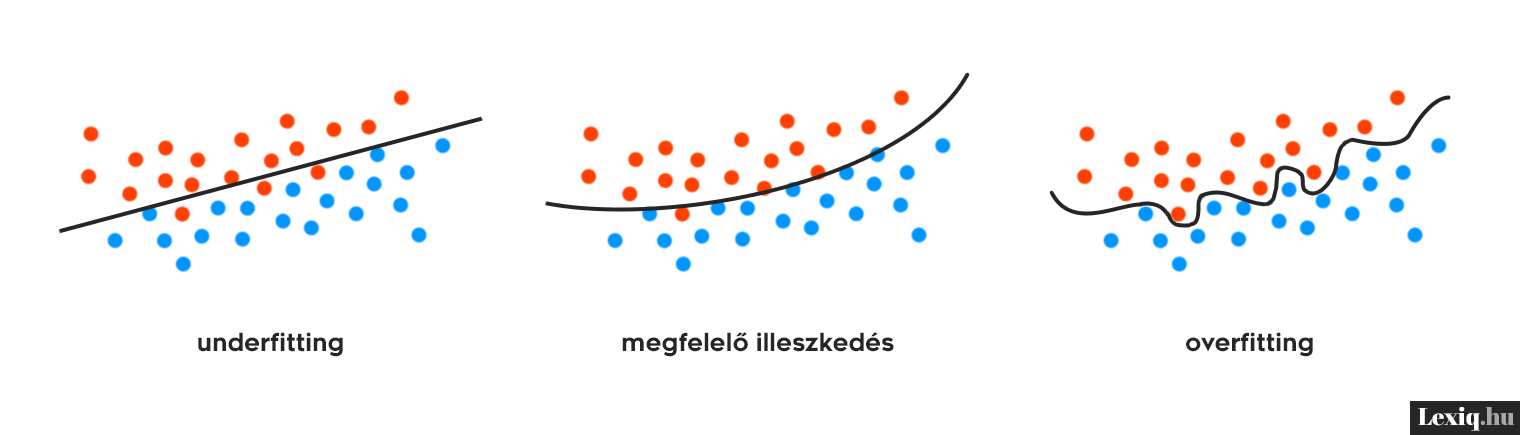
\includegraphics[width=12cm]{images/overfitting-abrazolasa.png}
	\caption{Overfitting ábrázolása egy adathalmazon\cite{overfitting}}
\end{figure}


\subsection{Adatfelosztásos validáció (split-validation)}
\label{subsec-split-validation}
A tanító készlet általában az összes adat 70-80 míg a tesztelő 20-30 százalékát jelenti. Míg a tanító készletet arra használjuk, hogy betanítsuk a modellt, a tesztelő készletet arra, hogy a modell pontosságát mérni tudjuk.

\subsection{K-szoros keresztvalidáció (k-fold cross validation)}
\label{subsec-cross-validation}
Itt az adatkészletet csakugyan elosztjuk $k$ egyenlő részre (fold), amiből 1 lesz a tesztkészlet\footnote{A $k$ részből egynél több is szolgálhat tesztkészletként}. Így tehát a $k-1$ darab tanító készleten betanítjuk, majd az így kapott modellt, ezen a maradék 1 készleten leteszteljük. Ezt az eljárást addig ismételjük, amíg az összes készletet fel nem használjuk tanító és tesztkészletként egyaránt. Az így kapott eredményeket ezután összesítjük és ennek átlagát vesszük, így egy átfogó értékelést alkotunk a modell teljesítményéről. Ez az átlagolt érték adja meg, hogy a modell általánosítási képessége várhatóan milyen lesz ismeretlen adatokon. Ezen kívül, a különböző iterációk során kapott eredmények szórása is fontos információkat szolgáltathat a modell stabilitásáról és megbízhatóságáról.\footnote{Amikor a tesztkészlet mindössze egyetlen elemből áll, akkor ezt \emph{Leave-One-Out Cross-Validation} (LOOCV) néven ismerjük, míg a \emph{Leave-P-Out Cross-Validation} (LPOCV) esetén a tesztkészlet $P$ elemű, ahol $P>1$.} Ez több számítási kapacitást igényel, viszont elkerüljük a túlilleszkedést (lásd \ref{sec-tulilleszkedes}. fejezet).


\section{Algoritmusok kiértékelése, összehasonlítása és metrikák}
\label{sec-algoritmusok-kiertekelese}
\subsection{Pontossági mérőszámok}
Számos algoritmus áll rendelkezésre, hogy megkapjunk egy mérőszámot mely az ajánló rendszerünk pontosságát tükrözi, ebből bemutatok néhányat.
Ebben az alszekcióban lévő egyenletekhez felhasznált irodalom: \cite{szupercella:elorejelzesek-verifikacioja, surpriselib:accuracy-module}


A matematikai formulákban lévő jelölések:
\begin{itemize}
	\item  $n$ jelöli a tesztkészletben lévő \emph{elemek számát},
	\item $x$ a \emph{megfigyelt értékek}, azaz a felhasználók által adott értékelések, $x_{i}$ az $i$-edik megfigyelt érték,
	\item $y$ a rendszerünk által készített \emph{becsléseket}, $y_{i}$ az $i$-edik becslés.
\end{itemize}

\subsubsection{Hibák mérése}
Általánosságban elmondható az alábbi metrikákra, hogy  minél kisebb a kapott érték, annál pontosabb becsléseket készít a rendszerünk.
\paragraph{Átlagos hiba (ME)}
Angolul \emph{Mean Error (ME)} vagy \emph{Bias (B)}.

Vegyük a tesztkészletben lévő, a rendszerünk által készített becslések és a felhasználó által adott értékelések különbségét és ennek számítsuk ki áz átlagát.

\[ \mathbf{ME} = \mathbf{B} =  \frac{\sum^{n}_{i=1}(y_{i}-x_{i})}{n}\]

Ez a legegyszerűbb mérőszám. Nem méri a hiba abszolút értékét, tehát nullát úgy is el lehet érni, hogy pozitív és negatív irányba is eltérhet a becslésünk és a megfigyelés különbsége. Más szavakkal a rendszerünk túl- és alulbecsülheti az egyes elemeket.

\paragraph{Átlagos abszolút hiba (MAE)} 
Angolul \emph{Mean Absolute Error (MAE)}.

Vegyük a tesztkészletben lévő, a rendszerünk által készített becslések és a felhasználó által adott értékelések különbségének abszolút értékét, és ennek számítsuk ki áz átlagát.
\[ \mathbf{MAE} = \frac{\sum^{n}_{i=1}\left | y_{i}-x_{i}\right |}{n} \]

Az előző (ME) hibáját igyekszik korrigálni, tehát a különbségek abszolút értékét veszi, ezáltal minden eltérést hibának vesz, legyen az pozitív vagy negatív irányban, de ez az egyik hibája is egyben, nem mutatja, hogy alul vagy túlbecsültük az elemeket.

\paragraph{Átlagos négyzetes hiba (MSE)}
\label{p:MSE}
Angolul \emph{Mean Squared Error (MSE)}.

Vegyük a tesztkészletben lévő, a rendszerünk által készített becslések és a felhasználó által adott értékelések különbségének négyzetét, és ennek számítsuk ki áz átlagát.
\[ \mathbf{MSE} = \frac{\sum^{n}_{i=1}(y_{i}-x_{i})^{2}}{n}\]

Ez sem veszi figyelmen kívül hagyja, hogy alul- vagy túlbecsültük az elemeket. A négyzetre emelés miatt érzékenyebb a nagyobb eltérésekre.


\paragraph{Átlagos négyzetes hiba gyöke (RMSE)}
\label{p:RMSE}
Angolul \emph{Root Mean Squared Error (RMSE)}.

Vegyük a tesztkészletben lévő, a rendszerünk által készített becslések és a felhasználó által adott értékelések különbségének négyzetét, és ennek számítsuk ki áz átlagát, majd ennek vegyük a négyzetgyökét.
\[ \mathbf{RMSE} = \sqrt{\frac{\sum^{n}_{i=1}(y_{i}-x_{i})^{2}}{n}}\]

Ez az előző kifejezés (MSE) négyzetgyökeként értelmezhető. Az eredeti mennyiséggel (azaz a megfigyelt változóval) azonos mértékegységgel rendelkezik. Például ha:
\[x=[5,5,4,4,3,2,5] \text{ és } y=[2,5,3,2,1,5,1]\]
akkor
\begin{align*}
	& \mathbf{MSE} = 6.1429 \\
	& \mathbf{RMSE} = 2.4785
\end{align*}

\emph{RMSE} jobban tükrözi a tényleges átlagos hiba nagyságát az eredeti mértékegységben.

\subsubsection{Top-N Találati arány}
\label{subsubsec-hit-rate}
A \emph{találati arány} (hit-rate) eredetileg az üzleti teljesítmény mérőszáma, mely hagyományosan az értékesítésekhez kapcsolódik.\cite{wiki-hit-rate} 
Ezt a metrikát gyakran használják ajánlórendszerek teljesítményének a mérésére. A felső N találati arány (top-N hit rate) azt mutatja, hogy a rendszer által ajánlott tételek közül hány esetben szerepel legalább egy, felhasználó által előnyben részesített tételek között.\cite{recommendation-system-evaluation-metrics}

\paragraph{Számításának menete}
\begin{enumerate}
	\item \textbf{Adatok előkészítése}: Osszuk fel az adatkészletünket tanító és tesztelő készletekre. Az adatkészletből távolítsunk el \emph{egy darab}, a felhasználó által preferált elemet, ez lesz a tesztkészletünk\footnote{Leave-One-Out cross validation vagy LOOCV}.
	\item \textbf{Modell tanítása}: tanítsuk be az ajánlórendszert a tanítókészletet felhasználva.
	\item \textbf{Top-N ajánlások generálása}: A tesztkészlet minden felhasználójához generálunk egy top-N ajánlási listát.
	\item \textbf{Találatok számítása}: Vizsgáljunk meg minden felhasználót, hogy a tesztkészlet eleme megjelenik-e az ajánlott N termékben, ha igen, az egy \emph{találat} (hit).
\end{enumerate}\cite{article-evaulating-a-real-life-recommender-system}

Ha például van 100 felhasználónk és 90 felhasználónál szerepelt a  megfigyelt elem a \emph{legjobb 10} ajánlásban, akkor a Top-10 Hit Rate $90\%$-os.

\subsection{Viselkedési metrikák}
\label{subsec-viselkedesi-metrikak}
Léteznek úgynevezett viselkedési metrikák, melyek nem a pontosságot, hanem egyéb fontos tulajdonságait mutatja az ajánlórendszerünknek. Ebben a részben felhasználtam a \cite{10-metrics-to-evaluate-rec-and-ranking-systems} található információkat.

Ilyen metrikák például:
\begin{itemize}
	\item \textbf{Lefedettség} (coverage): Egy százalékos arány, mely azt mutatja meg hogy a tanító készletből mennyi elemet tud ajánlani a tesztkészleten.\cite{evaluation-metrics-for-rec-sys}
	\item \textbf{Diverzitás} (diversity): Azt méri, hogy mennyire változatosak az ajánlott elemek. Egy magas diverzitású ajánlórendszer széles választékot kínál, ami segíthet felfedezni új érdeklődési területeket, így növelve a felhasználói elégedettséget. A diverzitás növelése azonban csökkentheti az ajánlások relevanciáját, ezért fontos megtalálni az egyensúlyt.
	\item \textbf{Újdonság} (novelty): Magas újdonsággal azok az új, vagy hosszú farokban\footnote{A \emph{hosszú farok}ról bővebben \cite{wiki-hosszu-farok}} lévő termékek bírnak, amelyekkel kevés felhasználó lépett interakcióba, a népszerű termékeket viszont alacsony újdonsággal lehet jellemezni.\cite{journal-the-definition-of-novelty-in-rec-systems}
	\item \textbf{Véletlenszerű felfedezés} (serendipity): Ez a metrika arra utal, amikor a rendszer olyan elemeket ajánl a felhasználónak, amelyek nem csak relevánsak, hanem meglepőek is, azaz olyan tartalmakat, amelyeket a felhasználó valószínűleg nem talált volna meg magától, de mégis értékel. A számszerűsítésének legyegyszerűbb módja a top-N ajánlott cikk átlagos népszerűsége.\cite{linkedin:serendipity}
	\item \textbf{Lemorzsolódás} (churn) és \textbf{Reakciókészség} (responsiveness): A \emph{lemorzsolódás} azt méri, hogy új értékelések után, milyen gyakorisággal változnak az ajánlások. A \emph{reakciókészség} az ilyen változások sebességét mutatja. \cite{recommender-systems-machine-learning-metrics-and-business-metrics}
\end{itemize}

Ezeknél a mérőszámoknál nem lehet feketén-fehéren kijelenteni, hogy a nagyobb érték az jobb rendszert eredményez. Ezek úgymond az ajánlórendszerünk stílusát, szofisztikáltságát jellemzik. Fontos lehet, hogy az ajánlórendszerünk tudjon sokszínű ajánlásokat tenni, ugyanakkor ennek a mértékének a meghatározása főleg valós felhasználókon történő teszteléssel lehet meghatározni (lásd \ref{a/b-teszteles}. fejezet).

\subsection{Online A/B Teszt}
\label{a/b-teszteles}
Az \emph{A/B tesztelés} más néven kettős tesztelés (split testing vagy bucket testing) egy olyan módszer, melyet a \emph{felhasználók viselkedésének} kutatására használnak. Általában egy adott dolog (például termék, weboldal, ajánlórendszer, stb.) kettő (A/B) vagy több változat összehasonlítására szolgál, általában azért, hogy kiválasszuk, melyik verzió teljesít jobban a \emph{valós felhasználók viselkedése alapján}.\cite{wiki-a/b-testing}

Lépések:
\begin{enumerate}
	\item \textbf{Adatgyűjtés}: Mielőtt megnéznék, hogy a rendszerünk más verziója hogyan teljesít, érdemes lehet a jelenlegi állapotáról információkat gyűjteni.
	\item \textbf{Hipotézis felállítása}: Egy hipotézis megfogalmazása, hogy a változatok között melyik és miért lehet jobb, miért van szükségünk a fejlesztésre, módosításra.
	\item \textbf{Változatok létrehozása}: Készítsünk kettő vagy több változatot, melyek csak egy-egy dologban térnek el egymástól.
	\item \textbf{Kísérleti csoportok kiválasztása}: A változatokat véletlenszerűen kiválasztott csoportoknak mutatjuk be.
	\item \textbf{Adatgyűjtés az összes változatról}: Figyeljük meg a felhasználók viselkedésének változásait a különböző változatoknál.
	\item \textbf{Elemzés}: Megállapítjuk, hogy melyik változat teljesített jobban a hipotézisben megfogalmazott kiválasztott nézőpontok alapján.
	\item \textbf{Döntéshozatal}: Eldöntjük melyik verziót szeretnénk bevezetni.
\end{enumerate}\cite{a/b-testing-guide}

Mivel \emph{valós felhasználókon} teszteljük a termékünk különböző verzióit, teljesen objektívan tudunk döntést hozni a változtatást illetően. Ugyanakkor hogy ezek az eredmények megbízhatóak legyenek elengedhetetlen, hogy megfelelően válasszuk ki a kísérleti csoportjainkat valamint ha valóban a verziók csupán csak egy-egy dologban térnek el, akkor nehezebbé válik a komplexebb változtatások tesztelése.

\chapter{Specifikáció}
\section{Feladat specifikáció}
Egy olyan alkalmazást tűztem ki a szakdolgozatom céljául, amivel szeretném demonstrálni egy modern webalkalmazás felépítését, népszerű eszközök használatával, valamint különböző szolgáltatások együttműködését, hogy hogyan is kerülnek a felhasználók elé az ajánlórendszer által készített ajánlások, egy egyszerű \emph{filmajánló} példáján keresztül. A hangsúlyt szerettem volna az alkalmazás felépítésére helyezni, ezért ezt csak egy \emph{MVP}-nek\footnote{Minimum Viable Product (MVP): ``Minimálisan Életképes Terméket jelent. A legkisebb olyan funkcionalitással rendelkező termék vagy szolgáltatás, amelyre visszajelzést tudunk kapni a potenciális felhasználóktól, ugyanakkor még nem feltétlenül piacképes.''\cite{mvp-es-mme-jelentese}} nevezném, mintsem egy kész alkalmazásnak. Ezért hiányoznak belőle olyan funkcionalitások, mint például az admin jogosultság, felhasználó vagy film adatainak módosítása, filmek értékelése.

\section{Rendszerterv}
A \emph{rendszerterv} (system design) az a folyamat, ahol definiáljuk, mely feltételeknek kell megfelelnie az elkészült alkalmazásunknak és azt, hogyan tervezzük megvalósítani azt.\cite{wiki-system-design, the-complete-guide-to-system-design-in-2024}

Ez egy kritikus lépés, mert az online szolgáltatásoknál széles skálán mozoghatnak a felhasználók, akiket ki kell szolgálnunk. Előfordulhat, hogy weboldalunkat csak néhányan látogatják, de például, a \emph{Facebook napi felhasználóinak (daily active users) száma} 2.064 milliárd.\footnote{Forrás: \url{https://www.demandsage.com/facebook-statistics/}} A rendszertervünknek tehát döntő szerepe lesz abban, hogy milyen felhasználói élményt nyújtunk, mennyire állunk azok rendelkezésére, így tehát, hogy sikeres lesz a projektünk, vagy kudarcba fullad.

\subsection{Architektúra}
\label{subsec-architektura}
Az alkalmazásomhoz \emph{szolgáltatásorientált architektúrát} választottam. A \emph{szolgáltatásorientált architektúra} (angolul Service-Oriented Architecture, röviden SOA) egy programozási módszer, aminek lényege, hogy az egyes szolgáltatások egy hálózatban helyezkednek el, és egy protokoll (jelen esetben \emph{HTTP}) által meghatározott módon kommunikálnak. \emph{A szolgáltatások különálló egységek, amik távolról is, valamint egymástól függetlenül is elérhetők, használhatók, frissíthetők, újra kombinálhatók.}\cite{wiki-szolgaltatasorientalt-architektura} Ez nagyon hasznos, hiszen ha más kliensoldali technológiát szeretnénk használni (például egy másik népszerű választás az Angular vagy Vue.js), akkor nem kell drasztikus változtatásokat végeznünk a frontenden, elég, ha megírjuk az új szolgáltatást, és ahhoz hozzá kapcsoljuk a már meglévő backendet, de ugyanez elmondható az összes komponensre. Valamint ezek a komponensek külön-külön is skálázhatók, ha szükséges, például \emph{Kubernetes}\footnote{\url{https://kubernetes.io/}} használatával.

\begin{figure}[H]
	\centering
	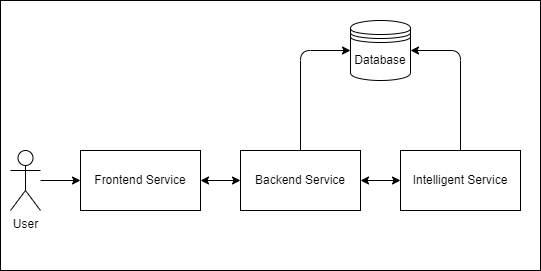
\includegraphics[width=14cm]{images/high-level-system-design.png}
	\caption[Magas szintű rendszerterv]{Magas szintű rendszerterv}
	\label{fig-rendszerterv}
\end{figure}

\Aref{fig-rendszerterv}.~ábrán igyekeztem egyszerűen szemléltetni a rendszerem tervét. A felhasználó (User) a \emph{Frontend Service}-szel (továbbiakban frontend vagy frontend szolgáltatás) van kizárólagos kapcsolatban. A frontend \emph{HTTP}\footnote{Éles környezetben biztonsági okokból érdemes \emph{HTTPS}-t használni.} protokollt használva kommunikál a \emph{Backend Service}-szel (továbbiakban backend vagy backend szolgáltatás), olyan kéréseknél mint például a bejelentkezés, regisztráció, ajánlások kérése. A backend kapcsolatban van az \emph{Intelligent Service}-szel (továbbiakban intelligens szolgáltatás), mely szolgáltatás feladata, hogy előállítsa az ajánlásokat a felhasználó részére, ez a kommunikáció is \emph{HTTP}\footnotemark[\value{footnote}] protokollon keresztül történnek. Mind a \emph{backend}, mind az \emph{intelligens szolgáltatás} kapcsolatban van az adatbázissal (Database), ahol a felhasználókról, filmekről, ajánlásokról tárolunk információkat (lásd \ref{subsec-adatbazis-terv}.~fejezet).

\subsection{Adatbázis terv}
\label{subsec-adatbazis-terv}
Az adatbázis megtervezésénél meg kell határozni, hogy milyen formában fogjuk tárolni az adatot, ez halmozottan fontos, ha strukturált adatbázist használunk, például PostgreSQL-t. \Aref{subsec-postgres}. fejezetben olvasható, miért a \emph{PostgreSQL} mellett döntöttem.

Egy meglévő, a \emph{GroupLens Research}\footnote{GroupLens Research hivatalos oldala: \url{https://grouplens.org}} által összegyűjtött adatkészletet, a \emph{MovieLens\footnote{MovieLens hivatalos oldala: \url{https://movielens.org}}}-t (azon belül is az \emph{ML latest small} adatkészletet) használom, ami eredetileg CSV (Comma-Separated Values) formátumban van tárolva, ezt PostgreSQL adatbázisba migrálom, tehát \emph{strukturált tabuláris adatot} alkalmazok. Ehhez a migrációhoz írtam pár Python szkriptet\footnote{A Python szkriptek megtalálhatók az \emph{applikáció/intelligent-service/data/scripts} mappában}.
\begin{itemize}
	\item \emph{separate-release-year-from-title.py}: Ezzel elkülönítem a \emph{title} részből a \emph{releaseYear}-t.
	\item \emph{generate-sql-script-to-create-dummy-users.py}: Létrehozunk egy \emph{sql} szkript fájlt, mellyel az adatbázist feltöltöm tesztelő felhasználókkal. Ezek nem valós felhasználói az alkalmazásnak, az adatkészletben a \emph{ratings.csv} fájlban az értékelésekhez van egy \emph{userId} társítva. Ez szükséges ahhoz, hogy tesztelhessük az alkalmazást.
	\item \emph{generate-sql-script-to-insert-data-into-movies-genres-and-movie-genres.py}: Ezt használva létrehozok egy \emph{sql} szkriptet, mely feltölti az adatbázist a \emph{movies.csv} fájlban található filmeket, műfajokkal.
	\item \emph{generate-sql-script-to-insert-data-into-ratings.py}: Végül a filmeket és felhasználókat felhasználva létrehozunk egy \emph{sql} szkriptet, ami az értékelésekkel egészíti ki az adatbázisunkat.
\end{itemize}

Ezekre a szkriptekre azért volt szükség, hogy \emph{harmadik normálformában} (3NF) tárolhassam az adatokat az adatbázisunkban (CSV fájlok helyett). A 3NF által csökkentjük az adatok redundanciáját, megakadályozzuk azok inkonzisztenciáját, javítjuk az adatintegritást, és optimalizáljuk a lekérdezések teljesítményét. Az így kapott adatbázis tervünk ER Diagramja\footnote{ER-modell: \url{https://hu.wikipedia.org/wiki/ER-modell}} látható a \ref{fig-er-diagram}.~ábrán.

\begin{figure}[H]
	\centering
	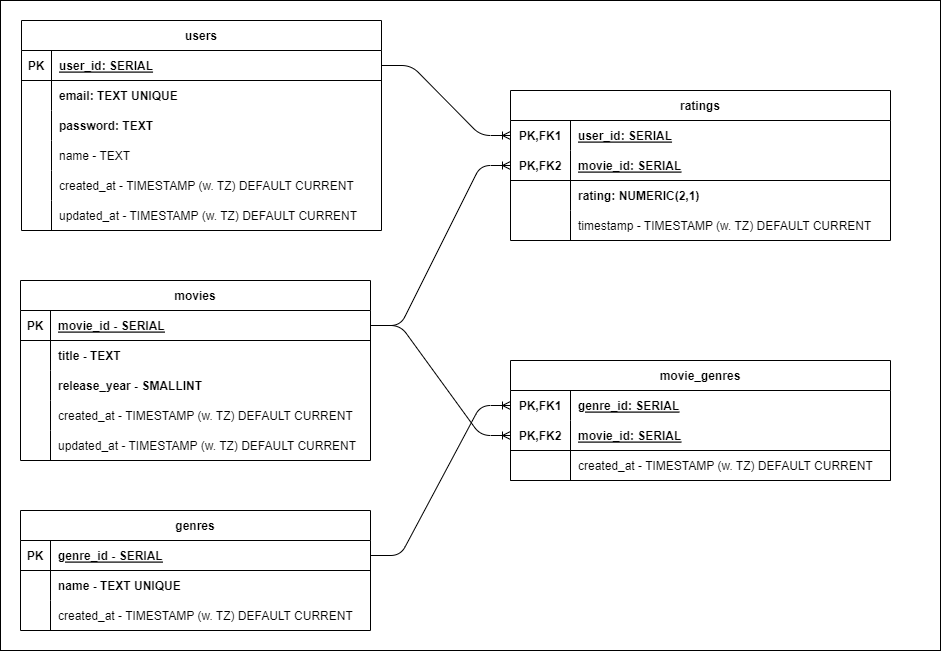
\includegraphics[width=14cm]{images/er-diagram.png}
	\caption[ER Diagram]{ER Diagram}
	\label{fig-er-diagram}
\end{figure}

\subsubsection{Felhasználók}
A felhasználókról csak a legfontosabb adatokat tároljuk, melyek elegendők azok megkülönböztetésére, azonosítására (autentikáció, lásd \ref{subsec-authentikacio-authorizacio}.~fejezet).

A regisztrációhoz, belépéshez kötelező megadni egy email címet (email) és egy jelszót (password) (amit majd hashelünk\footnote{``A hashelés azt a folyamatot jelenti, amelynek során egy változó méretű bemenetből egy fix méretű kimenetet állítunk elő.'' Forrás: \url{https://academy.binance.com/hu/articles/what-is-hashing}} és titkosítunk), valamint opcionálisan megadható egy felhasználónév (name). Nyomon szeretnénk követni, hogy mikor hozták létre (created\_at), valamint mikor módosították (updated\_at) utoljára a felhasználót. Minden felhasználóhoz szeretnénk hozzá társítani egy automatikusan létrehozott ID-t (user\_id), amit elsődleges kulcsként fogunk használni (Primary Key).

\begin{table}[!h]
	\centering
	\begin{tabular}{|l|c|c|c|} 
		\hline
		\textbf{Mező} & \textbf{Típus} & \textbf{Egyéb megkötés} \\ 
		\hline
		user\_id & SERIAL &  Primary Key \\ 
		\hline
		email & TEXT & Unique, Not Null\\ 
		\hline
		password & TEXT & Not Null \\ 
		\hline
		name & TEXT & -\\ 
		\hline
		created\_at & TIMESTAMP TZ\footnotemark\label{fn:table-tz-megfeleloje} & DEFAULT\_CURRENT \\ 
		\hline
		updated\_at & TIMESTAMP TZ\footnotemark[\value{footnote}] & DEFAULT\_CURRENT \\ 
		\hline
	\end{tabular}
	\caption{Felhasználók tábla}
	\label{tbl-users-table}
\end{table}
\footnotetext{TZ-t a ''WITH TIMEZONE`` rövidítésére használom helytakarékossági okokból}

\newpage

\subsubsection{Filmek}
A filmek (movies) tábla is mindössze a film címéből és a kiadásának évéből tevődik össze, ehhez is hozzárendeltem egy automatikusan létrehozott ID-t (movies\_id), amit elsődleges kulcsként fogunk használni valamint a létrehozásának és módosításának dátumát megörző (created\_at és updated\_at) mezőket.

\begin{table}[!h]
	\centering
	\begin{tabular}{|l|c|c|c|} 
		\hline
		\textbf{Mező} & \textbf{Típus} & \textbf{Egyéb megkötés} \\ 
		\hline
		movie\_id & SERIAL &  Primary Key \\ 
		\hline
		title & TEXT &  Not Null\\ 
		\hline
		release\_year & SMALLINT &  Not Null \\ 
		\hline
		created\_at & TIMESTAMP TZ\footnotemark[\value{footnote}] & DEFAULT\_CURRENT \\ 
		\hline
		updated\_at & TIMESTAMP TZ\footnotemark[\value{footnote}] & DEFAULT\_CURRENT \\ 
		\hline
	\end{tabular}
	\caption{Filmek tábla}
	\label{tbl-movies-table}
\end{table}

\subsubsection{Műfajok}
A műfajok (genres) táblában egy automatikusan létrehozott ID-t (genre\_id) és a létrehozásának dátumát (created\_at), valamint a műfaj megnevezését (name) tároljuk.

\begin{table}[!h]
	\centering
	\begin{tabular}{|l|c|c|c|} 
		\hline
		\textbf{Mező} & \textbf{Típus} & \textbf{Egyéb megkötés} \\ 
		\hline
		genre\_id & SERIAL & Primary Key \\ 
		\hline
		name & TEXT &  Not Null, Unique\\
		\hline
		created\_at & TIMESTAMP TZ\footnotemark[\value{footnote}] & DEFAULT\_CURRENT \\ 
		\hline
	\end{tabular}
	\caption{Műfajok tábla}
	\label{tbl-genres}
\end{table}
		
\subsection{Film Műfajok}
A filmek és műfajok közötti kapcsolatot a \emph{movie\_genres} táblában rögzítjük \emph{több-több} (many-to-many) kapcsolattal, mivel egy filmhez több műfaj is tartozhat, és egy műfajhoz több film is kapcsolódhat. Ez a tábla egy úgynevezett \emph{kapcsolótábla} (junction table), amely lehetővé teszi a filmek és műfajok közötti több-több kapcsolat reprezentálását. A genre\_id és a movie\_id is részét képzi az \emph{elsődleges kulcsnak} (Primary Key) valamint egy-egy \emph{idegen kulcsok} (Foreign Key) melyek a filmek és a műfajok táblákat kapcsolja hozzá ehhez a táblához.

\begin{table}[!h]
	\centering
	\begin{tabular}{|l|c|c|c|} 
		\hline
		\textbf{Mező} & \textbf{Típus} & \textbf{Egyéb megkötés} \\ 
		\hline
		genre\_id & INT & Primary Key, Foreign Key \\ 
		\hline
		movie\_id & INT & Primary Key, Foreign Key \\ 
		\hline
		created\_at & TIMESTAMP TZ\footnotemark[\value{footnote}] & DEFAULT\_CURRENT \\ 
		\hline
	\end{tabular}
	\caption{Felhasználók tábla}
	\label{tbl-movie_genres}
\end{table}

\subsubsection{Értékelések}
Az értékelések (ratings) tábla is egy \emph{kapcsolótábla} (junction table), mely \emph{több-több} (many-to-many) kapcsolatban köti össze a filmeket és a felhasználókat, akik értékelték azt. Itt a két genre\_id és a movie\_id együtt teszik ki az elsődleges kulcsot, valamint egy-egy idegen kulcsok. Ezen kívül tároljuk magát az értékelést 2 számjegyű formátumban, melyből egy a tizedes jegy, azaz  az értékek lehetnek 0.0-tól 9.9-ig (például 2.5 helyes, de 25 hibás). Tárolunk még egy \emph{timestamp} mezőt, ami az eredeti adatkészletből származik.

\begin{table}[!h]
	\centering
	\begin{tabular}{|l|c|c|c|} 
		\hline
		\textbf{Mező} & \textbf{Típus} & \textbf{Egyéb megkötés} \\ 
		\hline
		genre\_id & INT & Primary Key, Foreign Key \\ 
		\hline
		movie\_id & INT & Primary Key, Foreign Key \\ 
		\hline
		rating & NUMERIC(2,1) & Not Null \\ 
		\hline
		timestamp & TIMESTAMP & DEFAULT\_CURRENT \\ 
		\hline
	\end{tabular}
	\caption{Értékelések tábla}
	\label{tbl-ratings}
\end{table}


\subsection{Authentikáció}
\label{subsec-authentikacio-authorizacio}
Az \emph{autentikáció} az a folyamat, amely során egy felhasználó vagy rendszer igazolja saját identitását egy másik rendszer felé. Ez történhet többféle képpen, például az általunk használt email cím-jelszó párossal, vagy például digitális tanúsítvánnyal, biometrikus azonosítással is.\cite{wiki-authentication}

Az alkalmazásban első lépésként, a felhasználónak azonosítania kell magát az említett email cím-jelszó párossal. Ha az azonosítás sikeresen megtörtént, a backend létrehoz egy \emph{JWT tokent}\footnote{JWT-ről bővebben: \url{https://jwt.io/}}, mely tartalmazza a felhasználónk ID-ját. Majd létrehoz egy \emph{HttpOnly cookie}t, amiben eltárolja ezt a tokent. A \emph{HttpOnly cookie} azért biztonságosabb mint a ``hagyományos'' (nem HttpOnly) \emph{cookie} vagy egyéb tárolási mód, mert korlátozza a cookie-hoz való hozzáférését a kliensoldali szkripteknek. Ez növeli \emph{XSS}\footnote{XSS támadásról bővebben: \url{https://en.wikipedia.org/wiki/Cross-site_scripting}} támadások elleni védelmet. A \emph{HttpOnly cookie-nál} a cookie tárolja a:
\begin{itemize}
	\item nevét (name)
	\item értékét (value)
	\item domaint (domain)
	\item lejárat (expires / max age)
	\item útvonalt (path)
	\item lejárati dátumát (expires)
	\item méretét (size)
	\item egy boolean értékként, hogy HttpOnly cookie-e
	\item biztonságos-e (secure): ez annyit jelent, hogy HTTPS protokollt használva lett-e küldve, ami csökkenti a \emph{közbeékelődéses támadás}\footnote{Közbeékelődéses támadásról bővebben: \cite{wiki-kozbeekelodeses-tamadas}} (man-in-the-middle) kockázatát
	\item egy úgynevezett \emph{SameSite} mezőt, melynek értéke lehet: 
		\begin{itemize}
			\item \textbf{Strict}: Az alkalmazásban ezt választottam, mivel ez a Cross-site request forgery (CSRF)\footnote{CSRF-ről bővebben: \url{https://www.educative.io/answers/what-is-cross-site-request-forgery-csfr}} ellen óvja a felhasználót. Ezzel lényegében azt mondjuk a böngészőnknek, hogy csak a cookie-t beállító webhelyről származó kérésekben szerepeljen ez a cookie. 
			\item \textbf{Lax}
			\item \textbf{None}
			\item \textbf{Nem definiált}: Ebben az esetben \emph{Chrome 80-as verzójától} Lax értékként értelmezi a böngésző (olyan böngészőknél, melyek ezt a motort használják).
		\end{itemize} 
\end{itemize}

Ha ki szeretnénk jelentkezni, a \emph{backend} beállítja 0-ra a HttpOnly cookie \emph{maxAge} attribútumát, tehát a cookie azonnal le fog járni, így használhatatlan lesz a továbbiakban.

Ugyan az alkalmazásban csak ennyi autentikációt implementálok, érdemes megemlíteni pár másik nézőpontot. Az általam írt \emph{docker-compose.yml} fájl  \emph{fejlesztéshez} és \emph{teszteléshez} készült, ezért a dockeren kívül is elérhetőek a \emph{backend} és az \emph{intelligens szolgáltatás} API végpontjai. Éles környezetben azonban eldönthetjük, hogy az intelligens szolgáltatás végpontjait publikáljuk-e. Ha nem, akkor nincs is más dolgunk, mert a docker egy zárt környezet, de az ezen belül lévő konténerek tudnak egymással kommunikálni. Ellenkező esetben megfontolandó, hogy ezeket a végpontokon implementálunk autentikációt, autorizációt\footnote{Míg az autentikáció azt nézi, \emph{ki} végzi a műveleteket, az autorizációnál azt nézzük, hogy ennek az entitásnak \emph{van-e jogosultsága} az adott műveletek elvégzéséhez.}.


\chapter{Fejlesztés bemutatása}
Az ebben a fejezetben bemutatottak csak részletek vagy reprezentációk. Az alkalmazás megtalálható a \url{https://github.com/fepu08/szakdolgozat} GitHub tárolóban az \textbf{mvp} mappában. Minden esetben, ha hivatkozok egy forráskód fájlra (például \emph{./intelligent-service/app.py}) akkor az az \emph{mpv} mappától számított relatív útvonal.

\section{Intelligens szolgáltatás Benchmark modulja}
\label{sec-benchmark-modul}
A következő \ref{sec-hiperparameter-optimalizalas}. és \ref{sec-algoritmusok-osszehasonlitasa} fejezetekben az eltelt idő méréséhez, az intelligens szolgáltatásban implementáltam egy \emph{Benchmark}\footnote{Benchmark: számítógépes program, programkészlet vagy egyéb műveletek futtatása egy objektum relatív teljesítményének felmérése érdekében, általában számos szabványos teszt és próba futtatásával.\cite{wiki-benchmark}} modult, mely az alkalmazáson belül az \emph{./intelligent-service/utils/Benchmark.py} fájlban található. Az itt található \emph{TimeBenchmark} osztály használatával -- mely forráskódja \aref{code-timebenchmark-class}. kódban látható -- mérem az eltelt időt.

\lstinputlisting[style=python,caption=TimeBenchmark osztály,label=code-timebenchmark-class]{codes/benchmark-modul.py}

Ennek használata nagyon egyszerű, \aref{code-timebenchmark-hasznalata}. kódban látható.

\lstinputlisting[style=python,caption=TimeBenchmark használata,label=code-timebenchmark-hasznalata]{codes/time-benchmark-hasznalata.py}

Először is példányosítani kell a \emph{TimeBenchmark} osztályt (\ref{code-timebenchmark-hasznalata}. kód 1. sora), ami inicializálja a példány mezőit \emph{None} értékre (\ref{code-timebenchmark-class}. kód 2-5. sorai). Azért érdemes itt példányokat használni a statikus metódusokkal ellentétben, mert ha egyszerre több helyen szeretnénk mérni az időt megtehetjük, egymástól függetlenül, különböző példányokat használva. Így, mikor \aref{code-timebenchmark-hasznalata}. kód 2. sorában meghívjük a példány \emph{start} metódusát, az beállítja annak \emph{start\_time} mezőjének értékének az aktuális időt, Unix időbélyeg formájában.\footnote{Unix időbélyeg: 1970.01.1. 00:00:00 UTC óta eltelt másodpercek száma, lebegőpontos formátumban.} Ha be szeretnénk fejezni a mérést, akkor a példány \emph{stop} metódusát kell hívnunk (\ref{code-timebenchmark-hasznalata}. kód 6. sora). Ahogy \aref{code-timebenchmark-class}. kód 13. sorában olvasható, ez a példány \emph{end\_time} értékét fogja megadni Unix időbélyeg formájában ugyan úgy, mint a \emph{start} metódusnál. Majd a 14. sorban az \emph{end\_time} és a \emph{start\_time} értékeket kivonva, megadjuk a \emph{time\_elapsed} mező értékét, mely a \emph{start} és a \emph{stop} között eltelt időt mutatja. Ezt kiírathatjuk a \aref{code-timebenchmark-class}. kód 14. sorában levő \emph{print\_elapsed\_time} metódussal.

Ha újra szeretnénk indítani a mérést, megtehetjük a példány \emph{start} metódusának a meghívásával. Ilyenkor \aref{code-timebenchmark-class}. kód 8. sorában ellenőrizzük, hogy volt-e korábbi futtatás, a példány \emph{start\_time} mezőjének vizsgálatával, ha ez igaz értéket ad vissza, akkor meghívjuk az osztály privát \emph{\_\_clear} metódusát, mely \aref{code-timebenchmark-class}. kód 19-22. soraiban látható. Ez visszaállítja a példány mezőinek értékét a konstruktorban definiáltak szerint, azaz \emph{None}-ra.

\section{Hiperparaméter optimalizálás}
\label{sec-hiperparameter-optimalizalas}
A \emph{hiperparaméterekről} és azok optimalizálásáról a \ref{sec-ml-hiperparameter-optimalizalas} fejezetben már írtam, ennek implementálását szeretném bemutatni a \emph{Surprise} könyvtár használatával.

A \emph{Surprise} könyvtár lehetőséget biztosít \emph{hiperparaméter optimalizálásra} a \emph{GridSearchCV} és \emph{RandomizedSearchCV} nevű osztályok alkalmazásával. A szakdolgozatban az előbbit használom. Ez az osztály rácskereséses módszert használva az algoritmus pontossági mérőszámait számítja ki a hiperparaméterek különböző kombinációira, \emph{keresztvalidációt} (lásd \aref{subsec-cross-validation}. fejezetben) használva. Az implementáció megtalálható az \emph{./intelligent-service/hyperparameter\_optimization.py} elérési úton. Egy ahhoz hasonló kódrészlet látható az alábbi \ref{code-hyperparameter-tuning}. kódban. Referenciaként a dokumentációt használtam.\cite{surpriselib_docs:tune-algorithms-w-gridsearch}

\lstinputlisting[style=python,caption=Hiperparaméterek optimalizálása GridSearchCV használatával,label=code-hyperparameter-tuning]{codes/hyperparameter-tuning.py}

\Aref{code-hyperparameter-tuning}. kódban látható kódrészlet egy \emph{SVD} (lásd \aref{subsec-svd}. fejezetben) algoritmus számára keresi a legjobb paraméter párokat az 1-12. sorokban biztosított paraméterrács alapján. Ez az adatrács a modell különböző paramétereinek a lehetséges értékeit tartalmazza, mint például a faktorok száma (\emph{n\_factors}), vagy mint a tanulási ráta (\emph{lr\_all}). A 13. sorban példányosítjuk a \emph{GridSearchCV} osztályt. Ennek megadjuk paraméterként 
\begin{itemize}
	\item az algoritmust (\emph{SVD}),
	\item a paraméterrácsot (\emph{param\_grid}),
	\item a mérőszámokat, melyeket használ az összehasonlításokhoz (\emph{measures=["rmse", "mae"]}),
	\item a keresztvalidációhoz használt foldok számát (\emph{cv=5}).
\end{itemize}
Majd a 14. sorban található \emph{fit()} metódus minden paraméterkombinációra lefuttatja a vizsgálatot. Ehhez paraméterként egy \emph{surprise.dataset.Dataset} típusú adatkészletet kell biztosítanunk, mely az alkalmazásban a \emph{MovieLens ml-latest-small} (lásd \ref{subsec-adatbazis-terv}. fejezet) adatkészletből származik. \Aref{code-hyperparameter-tuning}. kód 16. sorában lévő kóddal megkaphatjuk a legjobb \emph{RMSE} (lásd \ref{p:RMSE} fejezet) pontszámot és a 17. sorban lévő kóddal az ehhez tartozó paramétereket. Ezeket a későbbiekben felhasználom.

Ugyanezekkel a paraméterekkel lefuttattam a keresést az \emph{MovieLens ml-latest-small} adatkészleten, és \aref{sec-benchmark-modul}. fejezetben leírt \emph{TimeBenchmark}-kal lemértem a futtatáshoz szükséges időt, ami \emph{21281.79} másodpercet vett igénybe, ami körülbelül \textbf{6 órának} felel meg!\footnote{\benchmarkSpecification{}} \Aref{fig-hyperparameter-tuning-task-manager}. ábrán látható, hogy nagyságrendileg a processzorból hány százalékot és a RAM-ból hány MB-ot vett igénybe a futtatás.

\begin{figure}[H]
	\centering
	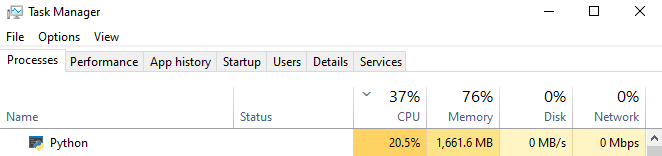
\includegraphics[width=14cm]{images/hyperparameter-tuning-grid-search.png}
	\caption[Hiperparaméter optimalizáció által igénybe vett erőforrások]{Hiperparaméter optimalizáció által igénybe vett erőforrások}
	\label{fig-hyperparameter-tuning-task-manager}
\end{figure}


\Aref{sec-algoritmusok-osszehasonlitasa}. fejezetben részletesebben ki fogok térni az algoritmusok összehasonlítására, azonban érdekességképpen lássuk, hogy az SVD vagy az optimalizált hyperparaméterekkel ellátott SVD (Tuned SVD) teljesít jobban \aref{fig-svd-vs-tuned-svd} ábrán.

\begin{figure}[H]
	\centering
	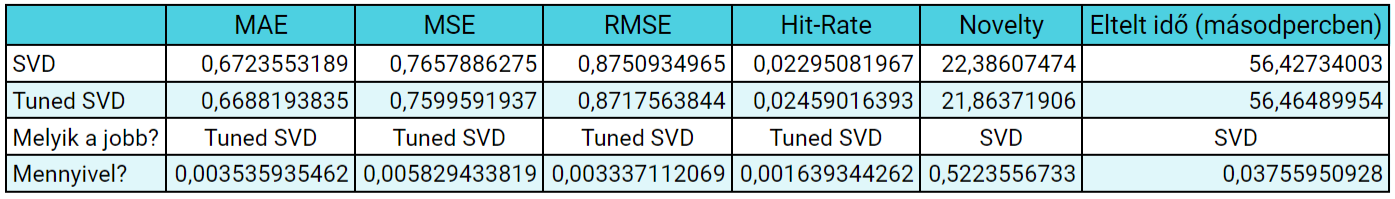
\includegraphics[width=14cm]{images/algoritmus-metrikak-svd-vs-tuned-svd.png}
	\caption[SVD és Tuned SVD összehasonlítása]{SVD és Tuned SVD összehasonlítása}
	\label{fig-svd-vs-tuned-svd}
\end{figure}


Nos, ahogy \aref{fig-svd-vs-tuned-svd}. ábra mutatja, a hiperparaméterekkel ellátott SVD (Tuned SVD) jobban teljesített, noha nem sokkal. Viszont érdemes figyelembe venni, hogy a használt adatkészlet megközelítőleg mindössze 600 felhasználó 9.000 filmre való 100.000 explicit értékelését tartalmazza.\footnote{Forrás: \url{https://grouplens.org/datasets/movielens/}} Ez közel sem mondható \emph{big datának} (big datáról \aref{sec-adat}. fejezetben találhatunk információkat). Lehet, a \emph{Netflix} vagy \emph{IMDb} adatbázisával ez a különbség sokkal számottevőbb lenne, noha jóval több mint 6 órába telne a futtatás.


\section{Algoritmusok összehasonlítása}
\label{sec-algoritmusok-osszehasonlitasa}
Ebben a részben \aref{subsec-surpriselib}.~fejezetben említett \emph{Surprise} könyvtárat használva kerülnek összehasonlításra az alábbi algoritmusok: 
\begin{itemize}
	\item \emph{random\_pred.NormalPredictor}: Az algoritmus a tanítókészlet eloszlásán alapuló véletlenszerű értékelés előrejelzésére.
	\item \emph{knns.KNNBasic}: Egy alap kollaboratív szűrési algoritmus.
	\item \emph{matrix\_factorization.SVD}: \Aref{subsec-svd}.~fejezetben említett SVD algoritmus.
	\item \emph{matrix\_factorization.SVD finomhangolt hiperparaméterekkel}: \Aref{sec-hiperparameter-optimalizalas}.~fejezetben kapott hiperparamétereket tápláltuk be az SVD algoritmusba.
	\item \emph{matrix\_factorization.SVDpp}: Az \emph{SVD++} algoritmus az \emph{SVD} kiterjesztése, mely figyelembe veszi az implicit értékeléseket.
\end{itemize}
Ezek mindegyike a \emph{Surprise} \emph{prediction\_algorithms} csomagjában vannak implementálva.\cite{surpriselib_docs:prediction_algorithms}

\Aref{sec-algoritmusok-kiertekelese}. fejezetben tárgyalt mérőszámokból párat fogunk vizsgálni, mégpedig:
\begin{itemize}
	\item \emph{MAE}
	\item \emph{MSE}
	\item \emph{RMSE}
	\item \emph{Hit-Rate} (Találati arány)
	\item \emph{Novelty} (Újdonság).
\end{itemize}
Ezek közül a \emph{MAE}, \emph{MSE} és az \emph{RMSE} implementálva van a \emph{Surprise} könyvtár \emph{accuracy} moduljában.\footnote{Surprise accuracy moduljának dokumentációja: \url{https://surprise.readthedocs.io/en/stable/accuracy.html}} A \emph{Novelty}-hez pedig egy \emph{recmetrics} nevű GitHub repositoryt valamint \emph{Claude Shannon} információtartalomra vonatkozó definícióját \cite{wiki-self-information} alkalmazom.\footnote{recmetrics novelty forráskódja: \url{https://github.com/statisticianinstilettos/recmetrics/blob/master/recmetrics/metrics.py\#L15}}

Ennek megvalósításához létrehoztam egy \emph{metrics} csomagot (package) az intelligens szolgáltatásban, ezen belül két modul található:
\begin{itemize}
	\item \emph{prediction\_evaluation}: Ebben egy \emph{Metrics} osztály van, amiben implementáljuk a metrikák kiszámítását a paraméterként átadott becslésekből.
	\item \emph{algorithm\_evaluation}: Itt egy \emph{AlgorithmEvaluator} osztály található, aminek feladata, hogy a biztosított algoritmusoknak a metrikáit kiértékelje a \emph{Metrics} osztály használatával. Ehhez elvégzi a szükséges adatok előkészítését és az eredmények kiíratásáról is gondoskodik.
\end{itemize}

\subsection{Újdonság (novelty) értékének kiszámítása}
\Aref{code-metrics-novelty} kódban látható egy kódrészlet az újdonság értékének kiszámításáról.

\lstinputlisting[style=python,caption=Újdonság értékének kiszámítása,label=code-metrics-novelty]{codes/novelty.py}

Ahogy \aref{code-metrics-novelty}. kód 6. sora mutatja, ez a statikus metódus két paramétert kér:
\begin{itemize}
	\item \emph{recommendations}: ez az algoritmus által generált Top-N ajánlási lista, egy \emph{defaultdict}\footnote{A \emph{defaultdict} egy szótár szerű adattípus, bővebben \url{https://docs.python.org/3/library/collections.html\#collections.defaultdict}} , melynél a kulcsok a felhasználó ID-k, az értékek \emph{listák} melyek elemei az ajánlott filmek ID-jából és a becsült értékelésekből készült \emph{tuple}\footnote{A \emph{tuple} egy vesszővel elválasztott értékekből álló adattípus (például \texttt{(1, "John Smith")}), bővebben: \url{https://docs.python.org/3/tutorial/datastructures.html\#tuples-and-sequences}}-ök.
	\item \emph{popularity\_rankings}: ez egy úgynevezett \emph{népszerűségi sorrend}\footnote{A népszerűségi sorrendet többféle képpen ki lehet számolni, ez a legegyszerűbb módja.}, egy \emph{defaultdict}, ahol a kulcsok film ID-k, az értéke pedig az előfordulásának a száma.
\end{itemize}

Az algoritmus a belső \emph{for} ciklusban (lásd \ref{code-metrics-novelty}. kód, 11-15. sorok) számítja ki az elemek információtartalmát, azaz azt, hogy egy adott elem előfordulása mennyire tekinthető valószínűtlennek (minél nagyobb az érték, annál valószínűtlenebb és váratlanabb az elem bekövetkezése). Ehhez \emph{Claude Shannon} információtartalomra vonatkozó definícióját alkalmazom.\cite{wiki-self-information}\footnote{Az információelméletben az információtartalom, öninformáció, meglepetés vagy Shannon-információ egy alapvető mennyiség, amely egy véletlen változóból származó különleges esemény bekövetkezésének valószínűségéből származik.} Ezt az elemenkénti információtartalmat \aref{code-metrics-novelty}. kód 15. sorában normalizálja a teljes elemszámot felhasználva. Majd a 18. sorban kiszámolja a rendszerre vonatkozó újdonságot, melyet az elemek átlagolásával kap meg. Ez a metódus, a 19. sorban két értéket ad vissza:
\begin{itemize}
	\item \emph{system\_level\_novelty}: A teljes rendszerre vonatkozó információtartalmat.
	\item \emph{mean\_self\_information}: Egy listát az elemenkénti információtartalommal.
\end{itemize}

\subsection{Találati arány (hit-rate) kiszámítása}
\Aref{code-hit-rate} kódban látható egy kódrészlet az újdonság értékének kiszámításáról.

\lstinputlisting[style=python,caption=Találati arány kiszámítása,label=code-hit-rate]{codes/hit-rate.py}

\Aref{subsubsec-hit-rate}. fejezetben már írtam a találati arány kiszámításáról, összefoglalva: a felhasználók által 1-1 preferált elemet kiválasztunk, ez lesz a tesztkészletünk, és megnézzük, hogy a rendszer által tett ajánlásokban milyen gyakran fordulnak elő ezek az elemek. Ugyan különböző módszerek vannak ennek kiszámítására, az egyszerűsége miatt azonban erre esett a választásom.

Ahogy \aref{code-hit-rate}. kód 4. sorában látható, ennek a metódusnak is két paramétert kell szolgáltatnunk, egy top-n ajánlást (\emph{top\_n\_recommendations}) és a tesztkészletet (\emph{LOOCV\_teststet})\footnote{LOOCV testset: a LOOCV a Leave-One-Out-Cross-Validation rövidítése, és ez annak a tesztkészlete, azaz a felhasználókhoz társított 1-1 elem.}. A 8. sorban ellenőrzi, hogy érvényes-e a teszkészletünk, ha nem, a 9. sorban egy nem informatív \emph{None} értéket ad vissza, de itt hibát is dobhatnánk. A \emph{for} ciklusban, \aref{code-hit-rate}. kód 11-14. soraiban számolja a találatokat. Ehhez végigiterál a tesztkészleten, majd az iterációban lévő felhasználó ID-ját (\emph{user\_id}) és kihagyott film ID-ját (\emph{left\_out\_movie\_id}), valamint a 12. sorban, a felhasználó ID-ját használva kiszelektálja a felhasználóhoz tartozó ajánlásokat (\emph{predicted\_movies}). Ezt használva, a 13. sorban ellenőrzi, hogy a kihagyott film ID-ja szerepel-e az ajánlások között, ha igen, a 14. sorban a számlálóhoz (\emph{num\_of\_hits}) ad egyet. A metódus végén, a 16. sorban a kapott találatok számát elosztja a tesztkészlet elemeinek számával, és az így megkapott értéket adja vissza, mint találati arány.

\subsection{A kiértékelés}
A kiértékeléshez létrehoztam az említett \emph{algorithm\_evaluation} modult, benne az \emph{AlgorithmEvaluator} osztállyal, ami a megtalálható az \emph{./intelligent-service\allowbreak/metrics\allowbreak/algorithm\allowbreak\_evaluator.py} elérési úton.

\lstinputlisting[style=python,caption=AlgorithmEvaluator osztály felépítése,label=code-algorithm-evaluator-high-level]{codes/evaluator-high-level.py}

\Aref{code-algorithm-evaluator-high-level}. kódban látható, hogy hogyan is épül fel ez az \emph{AlgorithmEvaluator} osztály. Példányosításkor biztosítanunk kell számára egy \emph{DataHandler} példányt, ami majd a szükséges adatokat fogja számára szolgáltatni, valamint a 11. sorban a konstruktorban létrehoz magának egy \emph{TimeBenchmark} példányt, amit a \emph{time\_benchmark} mezőjében tárol, ezzel foglyuk az eltelt időt mérni.

Az osztály tartalmaz 3 publikus
\begin{itemize}
	\item \emph{evaluate\_algorithms}: az paraméterként kapott algoritmusoknak végzi el a kiértékelését, kiíratja és CSV formátumban menti,
	\item \emph{print\_metrics}: kiírja a paraméterként kapott metrikákat ,
	\item \emph{save\_metrics\_to\_csv}: CSV formátumban menti a paraméterként kapott metrikákat a biztosított elérési útra
\end{itemize}
és egy privát \emph{\_\_prepare\_metrics} metódust mely egy segéd funkcióul szolgál, a paraméterként kapott metrikákból csinál egy \emph{pandas.DataFrame}-et.

\lstinputlisting[style=python,caption=EvaluateAlgorithms metódus,label=code-evaluate-algorithms-method]{codes/evaluator-evaluate-algorithms.py}

\Aref{code-evaluate-algorithms-method}. kód 10. sorában látható az \emph{evaluate\_algorithms} metódus, a következő paramétereket várja:
\begin{itemize}
	\item \emph{algorithms}: Egy szótár, amely tartalmazza a vizsgálni kívánt algoritmusokat és azok nevét.
	\item \emph{top\_n}: Egy logikai érték, amelynek alapértelmezett értéke igaz; ha igaz, elvégzi a \emph{hit-rate} és \emph{novelty} értékek kiszámítását és az ehhez szükséges műveleteket.
	\item \emph{n}: A \emph{top-n} ajánlás \emph{n} értékét határozza meg, alapértelmezett értéke 10.
	\item \emph{print\_result}: Egy logikai érték, amely ha igaz, kiírja a folyamat végén kapott metrikákat, alapértelmezett értéke igaz.
	\item \emph{save\_results}: Egy logikai érték, amely ha igaz, CSV fájlba írja a folyamat végén kapott metrikákat, alapértelmezett értéke igaz.
	\item \emph{save\_to}: Megadja, hova mentse a CSV fájlt, alapértelmezett értéke \emph{comparing-algorithms.csv}.
\end{itemize}

Az algoritmusok vizsgálata a 12-40. sorokban lévő \emph{for} iterációban történik. A 17. sorban betanítja az aktuális iterációban lévő modellt a \emph{self.data\_handler.get\_trainset()} által biztosított  adatfelosztásos validáció (\ref{subsec-cross-validation}. fejezet) tanító készletével. Majd a 18. sorban a már betanított algoritmustól készíttet egy ajánlókészletet a  \emph{self.data\_handler.\allowbreak{}get\_testset()} által kapott, a tanítókészlethez tartozó tesztkészletet felhasználva. A \emph{MAE}, \emph{MSE}, \emph{RMSE} kiértékeléséhez az egyszerűség és a gyorsaság végett használok adatfelosztásos validációt pl. keresztvalidáció helyett, melyeket a 20-22. sorokban ki is értékeljük ezeket, a már említett \emph{metrics.prediction\_evaluation} modult használva. A 23. soron ezeket meg is adja majd végeredményként szolgáló \emph{metrics} változóban.
\Aref{code-evaluate-algorithms-method}. kód 25-36. soraiban történik a \emph{Novelty} és \emph{Hit-Rate} értékek kiszámítása. Ehhez a 26. soron látható módon, az algoritmusunkat most a \emph{self.data\_handler.get\_leave\_one\_out\_\allowbreak{}trainset()} hívásával kapott \emph{Leave-One-Out-Cross-Validation} (LOOCV) tanító készletével tanítja be. Az \emph{LOOCV} egyrészt elengedhetetlen a \emph{Hit-Rate} kiszámításához, másrészt maximalizáljuk a tanítókészletet, mivel felhasználónként csak egy elemet hagyunk ki, ugyanakkor fennáll a veszélye a \emph{túlilleszkedésnek} (lásd \ref{sec-tulilleszkedes}. fejezet). A 27. sorban a \emph{test()} metódussal az \emph{LOOCV} tesztkészletét használva kiértékeli az algoritmus teljesítményét, úgy hogy előrejelzéseket készít a \emph{tesztkészletben lévő minden felhasználó-film párosra} és visszaad egy listát mely tartalmazza a tényleges és becsült értékeket is. A 28. sorban nagyjából ugyanezt hajtja végre, kivéve, hogy a \emph{self.data\_handler.get\allowbreak\_leave\allowbreak\_one\allowbreak\_out\allowbreak\_anti\allowbreak\_testset()} egy olyan adathalmazt, úgynevezett \emph{anti-testset}-et\label{anti-testset} (a \emph{surprise} könyvtár így hivatkozik erre az adatkészletre) ad vissza, amely tartalmazza az összes lehetséges felhasználó-film párost, amelyek nem szerepelnek az eredeti értékelési adatkészletben. Ez azt jelenti, hogy ezek azok a felhasználó-elem párosok, amelyekre a felhasználó által még nem történt interakció, értékelés. Ez azért fontos, mert éles környezetben ilyen elemekre szeretnénk ajánlásokat készíteni (nem feltétlen szeretnénk eladni valakinek újra és újra ugyanazokat a termékeket, például könyvek esetén). A 30. sorban ezt az adatkészletet felhasználva választja ki a felhasználók számára a legjobbra becsült \emph{n} (alapértelmezett értéke 10) elemet. A 32. sorban elvégzi a \emph{hit-rate} kiszámítását, majd a 33. sorban az \emph{újdonságét}. \Aref{code-evaluate_algorithm_metrics}. kódban látható mindennek a felhasználása.


\lstinputlisting[style=python,caption=Algoritmusok kiértékelése,label=code-evaluate_algorithm_metrics]{codes/evaluate_algorithm_metrics.py}

\Aref{code-evaluate_algorithm_metrics}. kód 5. sorában példányosítjuk az \emph{AlgorithEvaluator} osztályt, majd a hiperparaméter optimalizálásból  (lásd \ref{sec-hiperparameter-optimalizalas}. fejezet) származó adatokat paramétereket láthatjuk a 6-17. sorokban, melyeket majd egy \emph{SVD} algoritmusnak meg is adunk a 23-33. sorokban. A 19-35. sorokban látható, egy lista, mely elemei egy-egy szótár az algoritmusokkal és azok megnevezéseivel. Végül ezzel az \emph{algorithms} változóval meghívjük az \emph{evaluator.evaluate\_algorithms} metódusát a 37. sorban. Ennek eredményét láthatjuk \aref{fig-algoruitmus-metrikak}. ábrán.\footnote{\benchmarkSpecification} Ezt a metrikát felhasználva készítettem még másik két ábrát:
\begin{itemize}
	\item \Aref{fig-algoruitmus-metrikak-leggyorsabb-leglassabb}. ábrán látható  a leggyorsabban és leglassabban lefutott algoritmusok
	\item \Aref{fig-algoruitmus-metrikak-legjobb-ertekek}. ábrán látható  az egyes vizsgálatokon legjobban teljesített algoritmusok.
\end{itemize}


\begin{figure}[H]
	\centering
	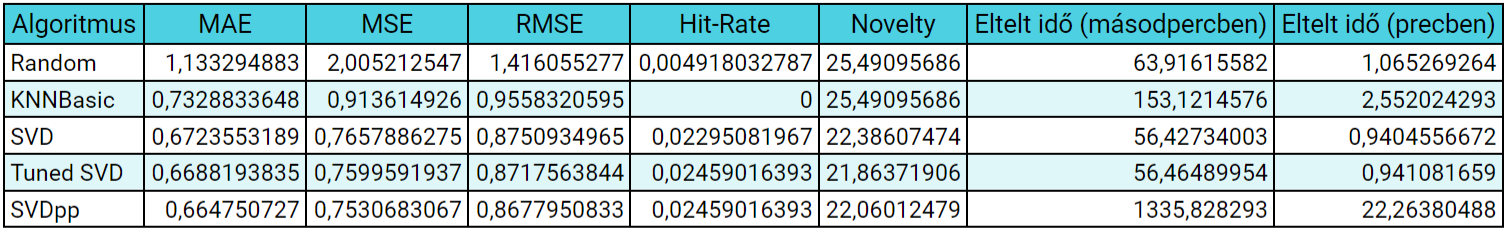
\includegraphics[width=14cm]{images/algoritmus-metrikak.png}
	\caption[Algoritmus metrikák és azok összehasonlítása]{Algoritmus metrikák és azok összehasonlítása}
	\label{fig-algoruitmus-metrikak}
\end{figure}

\begin{figure}[H]
	\centering
	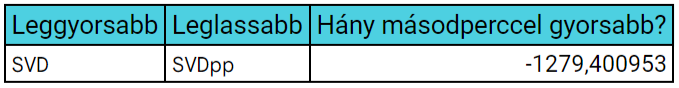
\includegraphics[width=8cm]{images/algoritmus-metrikak-leggyorsabb-vs-leglassabb.PNG}
	\caption[Algoritmus metrikák és azok összehasonlítása - Leggyorsabb és leglassabb vizsgálatok]{Algoritmus metrikák és azok összehasonlítása - Leggyorsabb és leglassabb vizsgálatok}
	\label{fig-algoruitmus-metrikak-leggyorsabb-leglassabb}
\end{figure}

\begin{figure}[H]
	\centering
	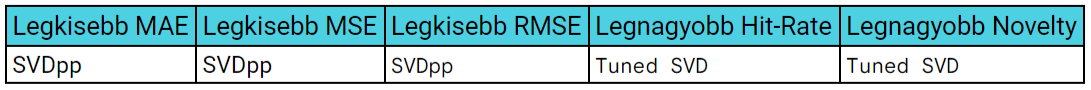
\includegraphics[width=10cm]{images/algoritmus-metrikak-legjobb-ertekek.png}
	\caption[Algoritmus metrikák és azok összehasonlítása - legjobb értékek]{Algoritmus metrikák és azok összehasonlítása - legjobb értékek}
	\label{fig-algoruitmus-metrikak-legjobb-ertekek}
\end{figure}

Az \emph{SVDpp} az \emph{SVD} egy változata, mely értékesíti az implicit értékeléseket. Noha az általunk választott adatkészletben kizárólag explicit értékelések vannak, mégis az \emph{SVDpp} kapta a legjobb értékeléseket, még ha nem is sokkal.

\section{Adatok tárolása és manipulálása}
\label{sec-adatok-tarolasa-es-manipulalasa}
Az alkalmazáshoz \emph{MovieLens ml-latest-small} (lásd \ref{subsec-adatbazis-terv}. fejezet) adatkészletét használom, mely eredetileg \emph{CSV}\footnote{CSV: \emph{Comma-Separated-Values} azaz vesszővel elválasztott értékek. Egy szöveges fájl, melyben az adatok vesszővel (vagy más előre definiált karakterrel például pontosvesszővel vannak elválasztva), ezzel biztosítva egy tabuláris adatstruktúrát.} formátumban vannak tárolva (például lásd \aref{code-ratings-csv-example}. kódot).

\lstinputlisting[style=python,caption=ratings.csv első sorai,label=code-ratings-csv-example]{codes/ratings.csv}

Az intelligens szolgáltatás fejlesztése elején, ezeket a \emph{CSV} fájlokat használtam adatforrásként, de később, hogy az adatok a \emph{backend szolgáltatás} rendelkezésére is elérhetők legyenek, valamint hogy demonstráljam egy általános webalkalmazás architektúráját az adatokat \emph{PostgreSQL} adatbázisba migráltam (bővebben \aref{subsec-adatbazis-terv}. fejezetben). Mindez jó példa arra, hogy az adatforrás egy alkalmazás élettartalma alatt változhat, ezt érdemes észben tartani, mikor megtervezzük a szoftverünket.

Mindennek a megvalósításához jó hasznát vesszük a \emph{függőség megfordításának elvének} (Dependency Inversion Principle vagy DIP), mely kimondja, hogy:
\begin{itemize}
	\item A magas szintű kód nem függ az alacsonyabb szintűtől, mindkettő az absztrakciótól függ.
	\item Az absztrakció nem a részletektől függ, hanem a részletek függnek az absztrakciótól.
\end{itemize}\cite{wiki-dip-magyar} 
Erről látható egy \emph{UML} diagram \aref{fig-dip-general}. ábrán:
\begin{itemize}
	\item A magas szintű kódot a \emph{HighLevelClass} reprezentálja, mely az absztrakciótól, azaz  \emph{BaseInterface}-től függ.
	\item Nem az absztrakció (\emph{BaseInterface}) függ a részletektől (\emph{ConcreteClass1} és \emph{ConcreteClass2}), hanem fordítva.
\end{itemize}

\begin{figure}[H]
	\centering
	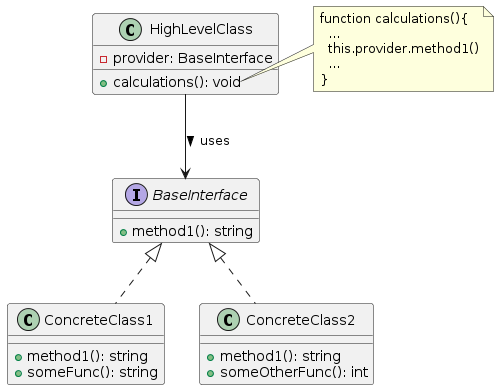
\includegraphics[width=10cm]{images/dip-general.png}
	\caption[Függőség megfordításának elvének bemutatása UML diagramon]{Függőség megfordításának elvének bemutatása UML diagramon}
	\label{fig-dip-general}
\end{figure}

\subsection{Intelligens szolgáltatás}
A fent említett függőség megfordításának elvének implementálását láthatjuk az intelligens szolgáltatásban is \aref{fig-dip-intelligent-service}. ábrán látható módon\footnote{A Pythonban nincs a C\# nyelvhez hasonló \emph{interface}, ezért ezt egy osztállyal oldom meg.}. Az intelligens szolgáltatáson belül, az alkalmazáshoz kapcsolódóan minden szükséges adattal kapcsolatos funkcionalitást a \emph{DataHandler} osztályban tárolunk. Egy \emph{függőség befecskendezés} (dependency injection)\footnote{A \emph{függőség befecskendezése} (dependency injection) a számítógép-programozásban egy technika, aminek lényege, hogy egy objektum más objektumok függőségeit elégíti ki.\cite{wiki-dependency-injection-magyar}} történik, mikor példányosítjuk a \emph{DataHandler} osztályunkat, ugyanis egy \emph{DataProviderBase} típusú objektumot kell biztosítanunk a konstruktor egy paramétereként. Ezt a \emph{DataProviderBase} objektumot használjuk, mikor a \emph{DataHandler} konstruktorában lekérjük a \emph{movie\_data} és \emph{ratings\_data} mezők értékét.

\begin{figure}[H]
	\centering
	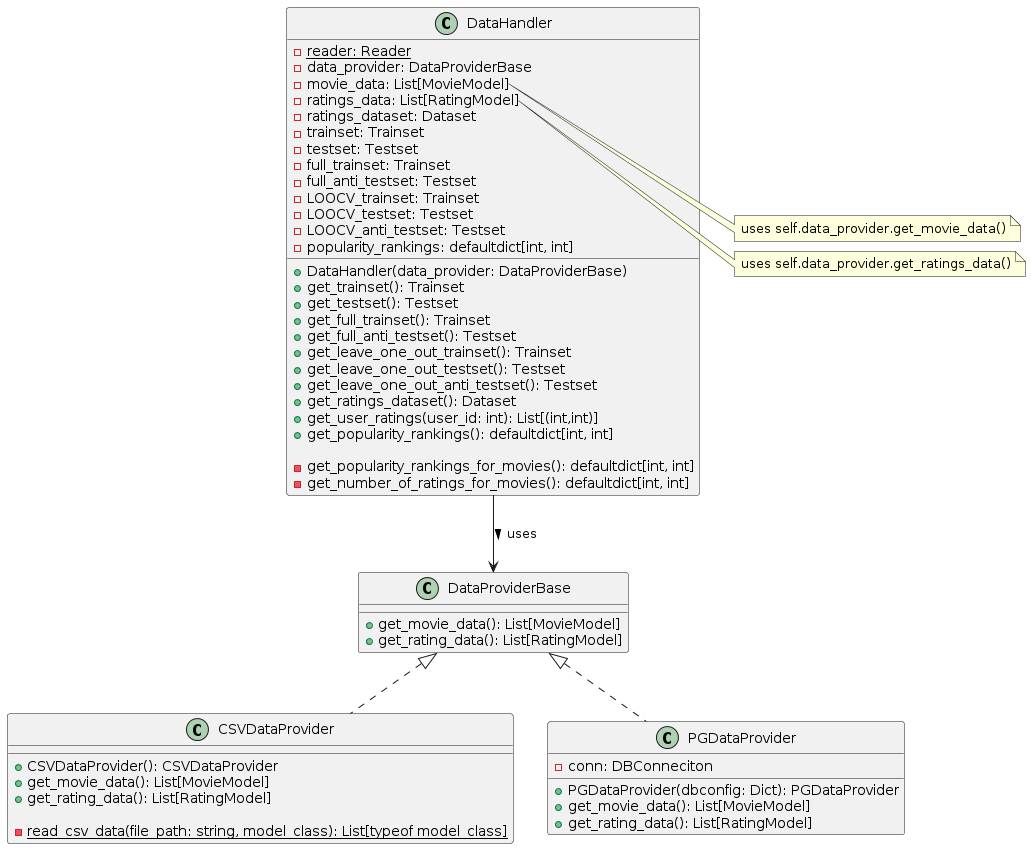
\includegraphics[width=14cm]{images/data-manipulation-in-intelligent-service.png}
	\caption[Függőség megfordításának elvének UML diagramon való bemutatása az intelligens szolgáltatásban]{Függőség megfordításának elvének bemutatása az intelligens szolgáltatásban UML diagramon}
	\label{fig-dip-intelligent-service}
\end{figure}

\Aref{code-dip-intelligent-service}. kódban látható, hogy hogyan használhatjuk a különböző \emph{DataProviderBase} implementációit a kódban.

\lstinputlisting[style=python,caption=DataHandler használata különböző DataProviderekkel,label=code-dip-intelligent-service]{codes/dip-intelligent-service.py}

\subsection{Backend szolgáltatás}
\subsubsection{Architektúra}
\label{subsubsec-backend-architektura}
Ahhoz, hogy megértsük, hogyan történik a \emph{backend szolgáltatás} és az \emph{adatbázis} közötti kommunikáció, nézzük meg egy részletét \aref{code-backend-src-folder-structure}. kódban látható \emph{src}\footnote{A \emph{backend szolgáltatásban} ebben a mappában tároljuk a forráskódokat.} mappa felépítéséről.

\lstinputlisting[style=python,caption=Backend szervíz \emph{src} mappájának tartalmáról egy részlet,label=code-backend-src-folder-structure]{codes/backend-src-structure-user-service.txt}

A szolgáltatásnál igyekeztem egy \emph{RESTful API}-t létrehozni, ami állapotmentes műveletek sorozatára épít meghatározott erőforrásokkal szemben. Noha a \emph{Richardson Maturity Model}\footnote{Forrás: \url{https://martinfowler.com/articles/richardsonMaturityModel.html}}-ből az utolsó, 3. szintnek nem teszek eleget, de ez nem is állt szándékomban. Továbbá figyelembe vettem, hogy az API legyen ellátva \emph{verzióval}, és a erőforrások jól elkülöníthetőek legyenek. Így tehát, ahogy az \aref{code-backend-src-folder-structure}. kódban a 2-14. sorokban is látható, azokat az \emph{src/api/v1} mappába rendeztem. Az erőforráson belül a különböző fájlok magyarázata a következő:
\begin{itemize}
	\item \emph{*-routes.ts}: A beérkező \emph{HTTP(S)} kérést irányítja a megfelelő erőforráshoz, hozzá társítva a kontrollert, és annak funkcióját.
	\item \emph{*-controller.ts}: A kontroller fogadja a felhasználói kéréseket és összekapcsolja azokat a megfelelő szolgáltatásokkal (services) vagy adatkezelő rétegekkel (DAO). Ebben a struktúrában a kontroller a kérés fogadásáért és válasz visszaküldéséért felelős.
	\item \emph{*-service.ts}: A \emph{service} réteg tartalmazza az üzleti logikát és a szükséges adatműveleteket, azaz a kérés feldolgozását végzi.
	\item \emph{*-dao.ts}: A \emph{DAO} (Data Access Object) a konkrét adatelérési logikát kezeli, tehát az \emph{adatbázisműveleteket} hajtja végre.
	\item \emph{*-dto.ts}: Az \emph{adatátviteli objektum} (DTO - Data Transfer Object) lényege, hogy egyszerűsítse és optimalizálja az adatok átvitelét különböző rendszerrészek között, minimalizálva ezzel a felesleges adatforgalmat és egyszerűsítve az adatstruk-\\túrákat.\cite{wiki-dto-hun}
	\item \emph{*-model.ts}: A \emph{Sequelize} használatához szükséges adatmodell definícióit tartalmazzák. Ezek leírják az adatbázis táblák szerkezetét, attribútumait és kapcsolatait, lehetővé téve a \emph{Sequaliz} számára, hogy \emph{ORM} (Object-Relational Mapping) módon kezelje az adatbázis-műveleteket.
\end{itemize}

\subsubsection{Adatbázissal való kommunikáció}
Az adatbázissal való kommunikációhoz a \emph{pg} és a \emph{sequelize} csomagokat használom. Az előbbit (pg) a \emph{PostgreSQL} adatbázishoz való kapcsolódásra míg az utóbbit (sequelize) az \emph{ORM} feladatokat ellátására alkalmazom. A \emph{sequelize} nem csak PostgreSQL, hanem más relációsadatbázis-kezelő rendszerekkel is működik. Minden erőforráshoz készítünk egy modellt, mely reprezentálja az adatbázis táblákat, ezt használja majd a \emph{sequelize} csomag. Ez egy kicsit kötöttebb felépítést biztosít, mivel ahhoz hogy más adatbázist használjunk, a \emph{./backend-service/src/config/sequelize-config.ts} számára más adatbázis klienst kell biztosítani. Ugyanakkor annak köszönhetően, hogy \aref{subsubsec-backend-architektura}. fejezetben bemutatott módon felosztottuk az erőforrásoknak egy-egy feladatát, az így kapott \emph{DAO}-kat már nem kell módosítani. Valamint \emph{DAO}-kat használva a \emph{service} réteg számára már nem számít, honnan származik az adat. Emellett, az egyes erőforrások tudnak kommunikálni egymással is, erre példa, mikor lekérjük a Top-N ajánlási listát a felhasználó számára, az a \emph{RecommendationService}-ből fogja használni a \emph{MovieService}-t, hogy a kapott film ID-khoz lekérje a filmek adatait.

\section{Az alkalmazás megtekintése}
Nézzük meg, hogyan is áll mindez össze egy egésszé. \Aref{fig-home-page}. ábrán az alkalmazásunk kezdőlapját láthatjuk, tesztelemekkel feltöltve. Igyekeztem egy \emph{streaming} szolgáltató (pl. Netflix) felületéhez hasonló egyszerűsített kezdőlapot létrehozni. Itt különböző kategóriákat láthatunk, úgy mint: 
\begin{itemize}
	\item ``New and Trending'': Új és népszerű filmek. Ezt az adatbázis lekérdezésével a legegyszerűbb meghatározni.
	\item ``Because you watched...'': Amiért megnézted a ... filmet, ajánljuk ezeket a filmeket. Ez egy jó példa \aref{subsec-kollaborativ}. fejezetben említett \emph{elem-alapú kollaboratív szűrők} felhasználására, például ha a felhasználó többször megnézte \emph{A Mátrix}ot (implicit adat), és ötből 5 csillagosra is értékelte (explicit adat), akkor az ehhez hasonló filmeket keressük. De ennek a megvalósítását nem mutatom be a szakdolgozatban.
	\item ``Action'': Különböző műfajokon belüli filmek, ebben a példában akciófilmek. Itt is lehetséges azt megcsinálni, hogy megnézzük a felhasználó által legnézettebb műfajt vagy műfajokat, és azokból ajánlunk más népszerű filmeket, vagy ezt is bővíthetjük még \emph{elem-alapú} szűrőkkel.
\end{itemize} 

\begin{figure}[H]
	\centering
	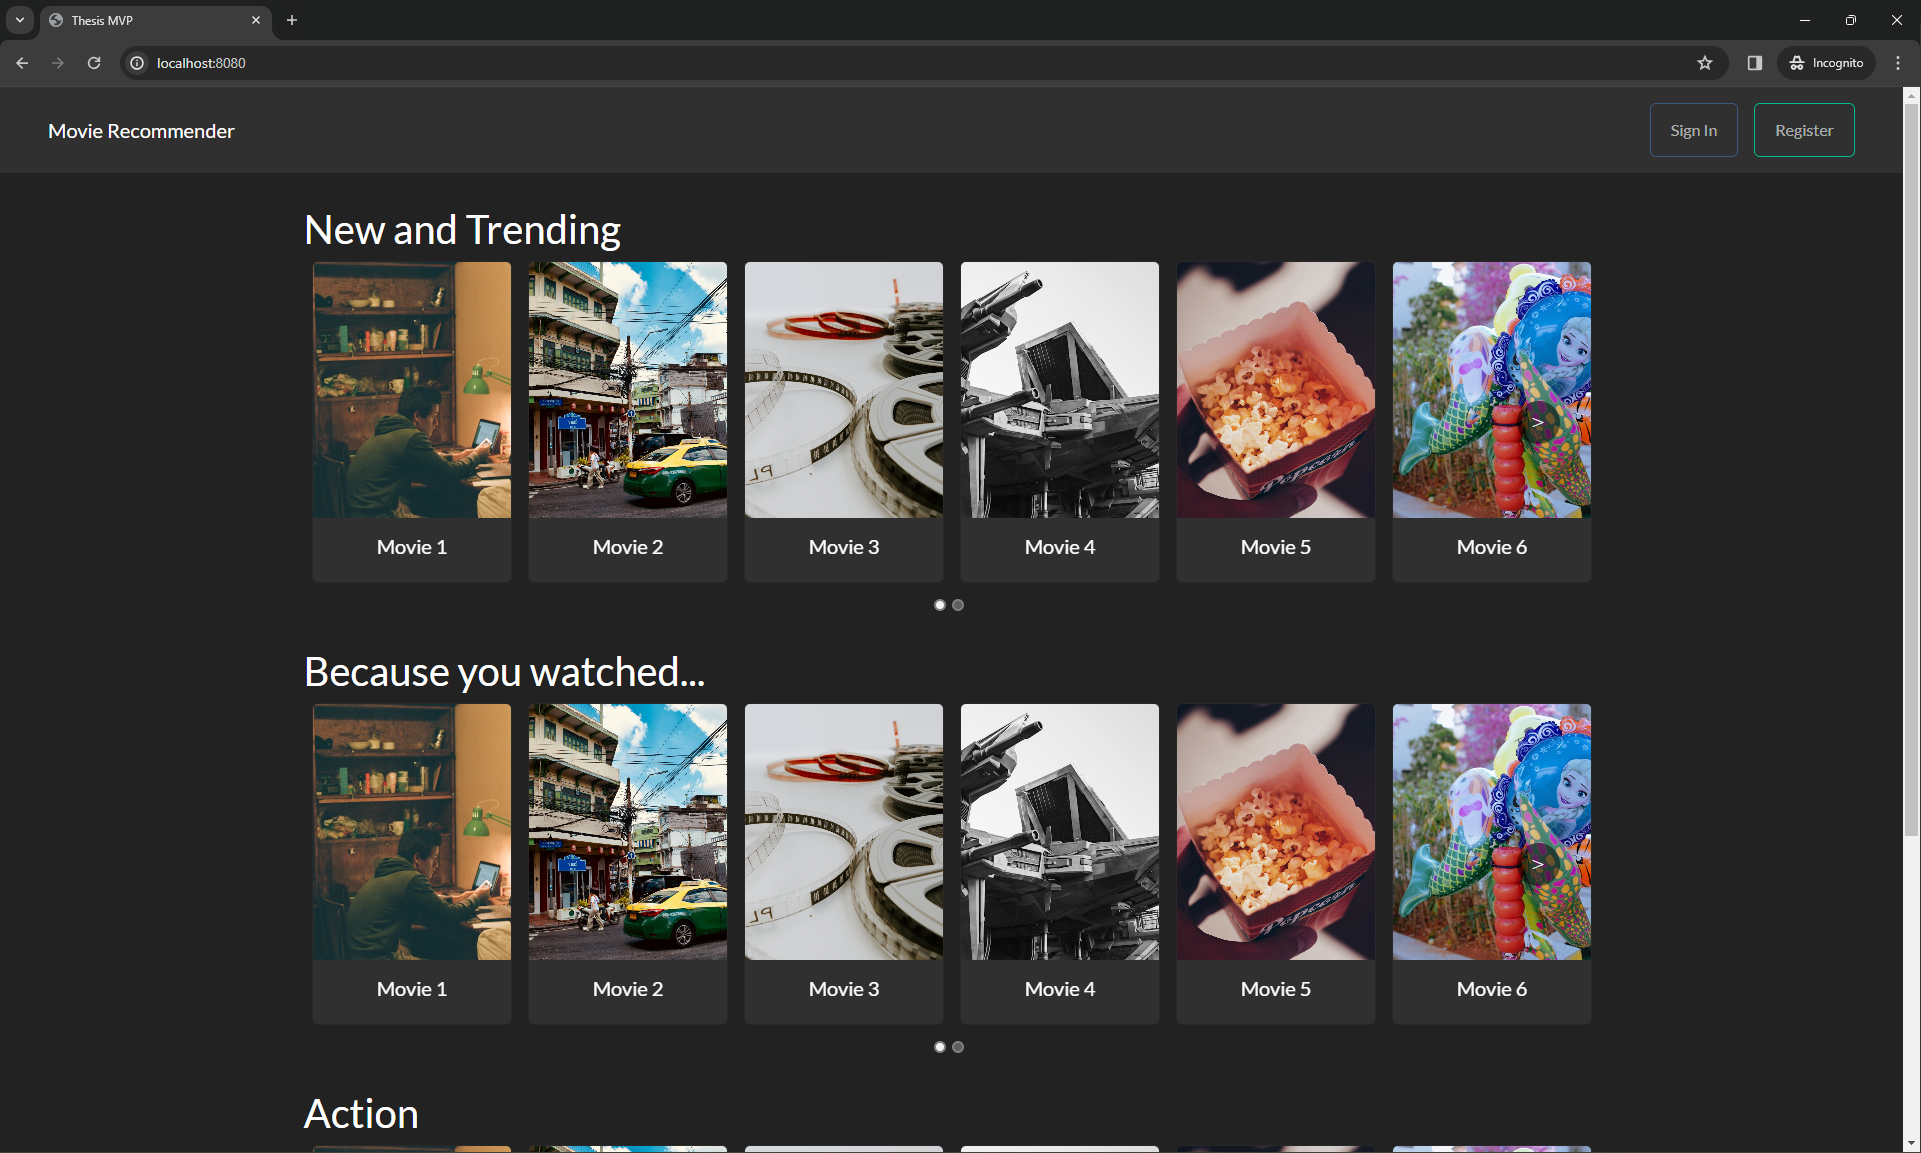
\includegraphics[width=14cm]{images/frontend-home-1.png}
	\caption[Az alkalmazás kezdőlapja]{Az alkalmazás kezdőlapja}
	\label{fig-home-page}
\end{figure}

\subsection{Autentikáció}
\label{demo-autentikacio}
\Aref{fig-home-page}. ábra jobb felső sarkában láthatjuk a \emph{Sign In} (bejelentkezés) és \emph{Register} (regisztráció) gombokat.

A \emph{Register} gomb megnyomása után a felület betölti a regisztrációs űrlapot, mely \aref{fig-register}. ábrán látható.

\begin{figure}[H]
	\centering
	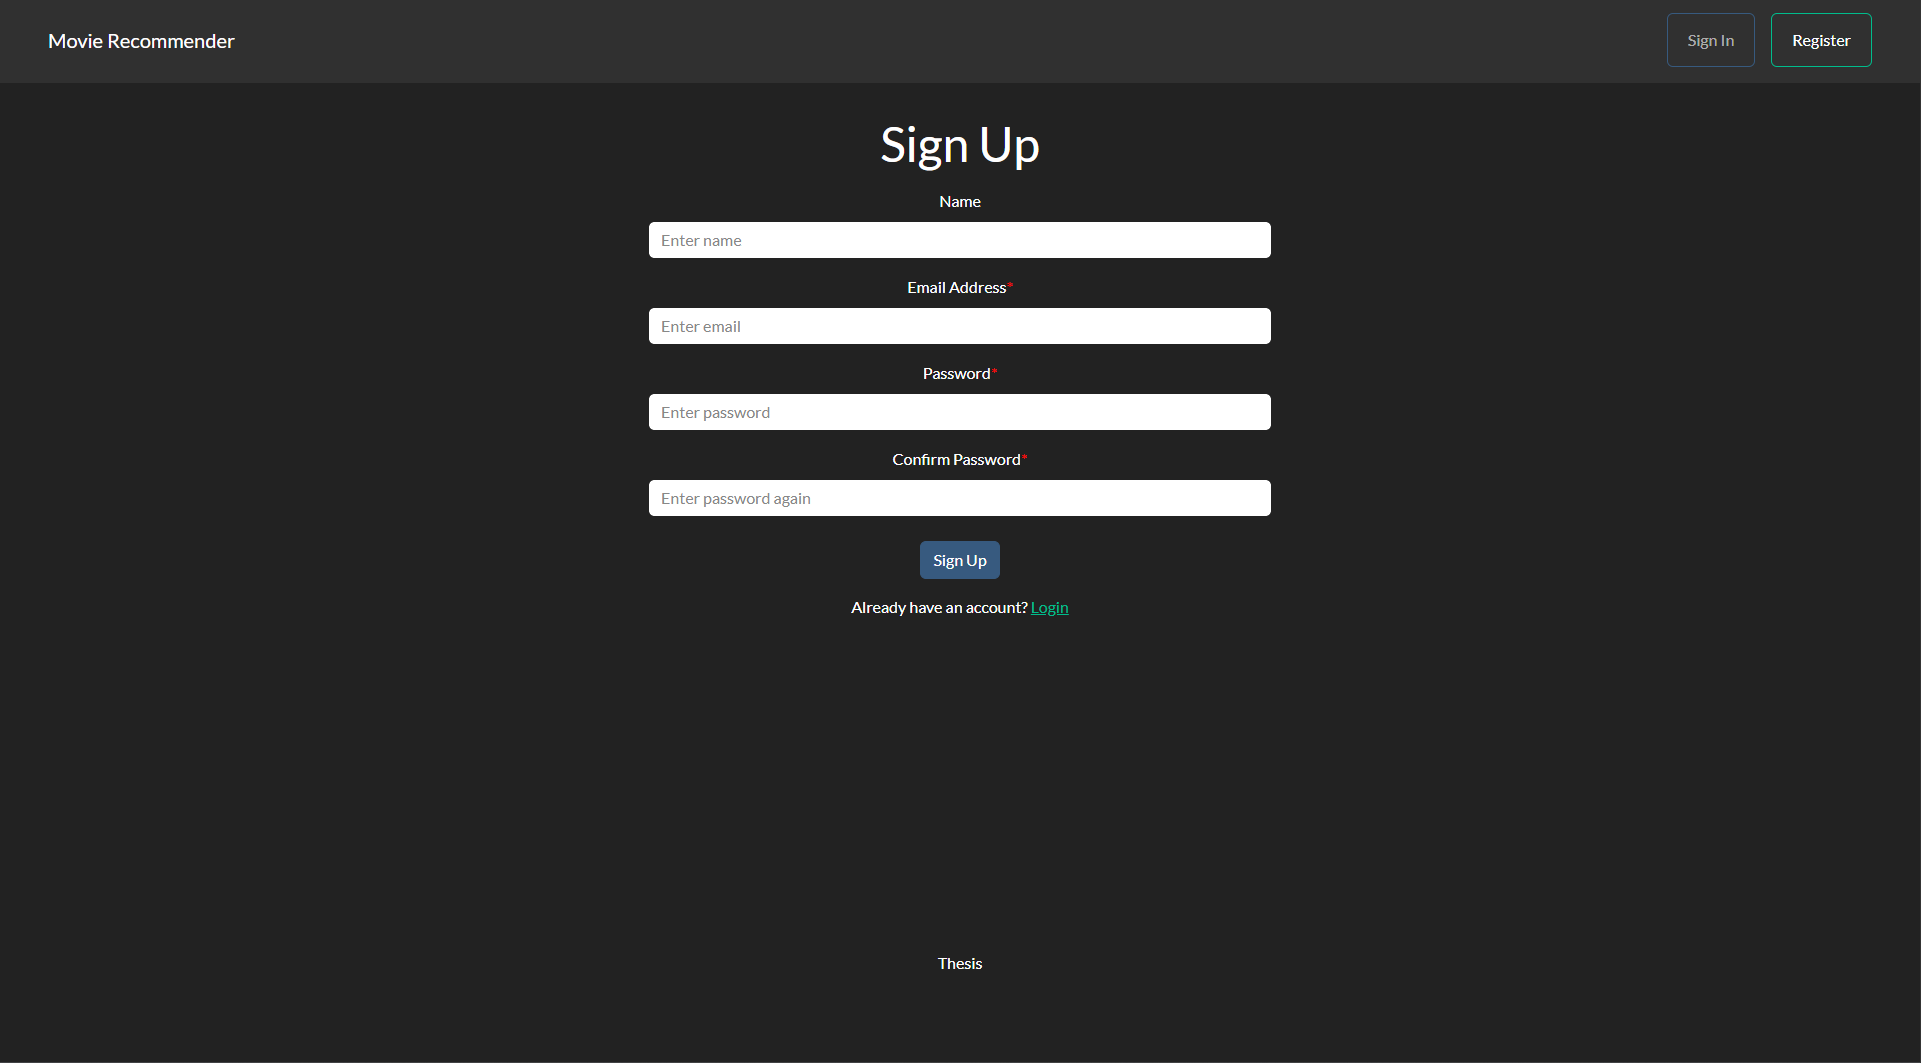
\includegraphics[width=14cm]{images/frontend-register-1.png}
	\caption[Regisztrációs felület]{Regisztrációs felület}
	\label{fig-register}
\end{figure}

Rendre a \emph{Sign In} gomb megnyomása után a felület betölti a bejelentkezési űrlapot (\ref{fig-sign-in}. ábra).

\begin{figure}[H]
	\centering
	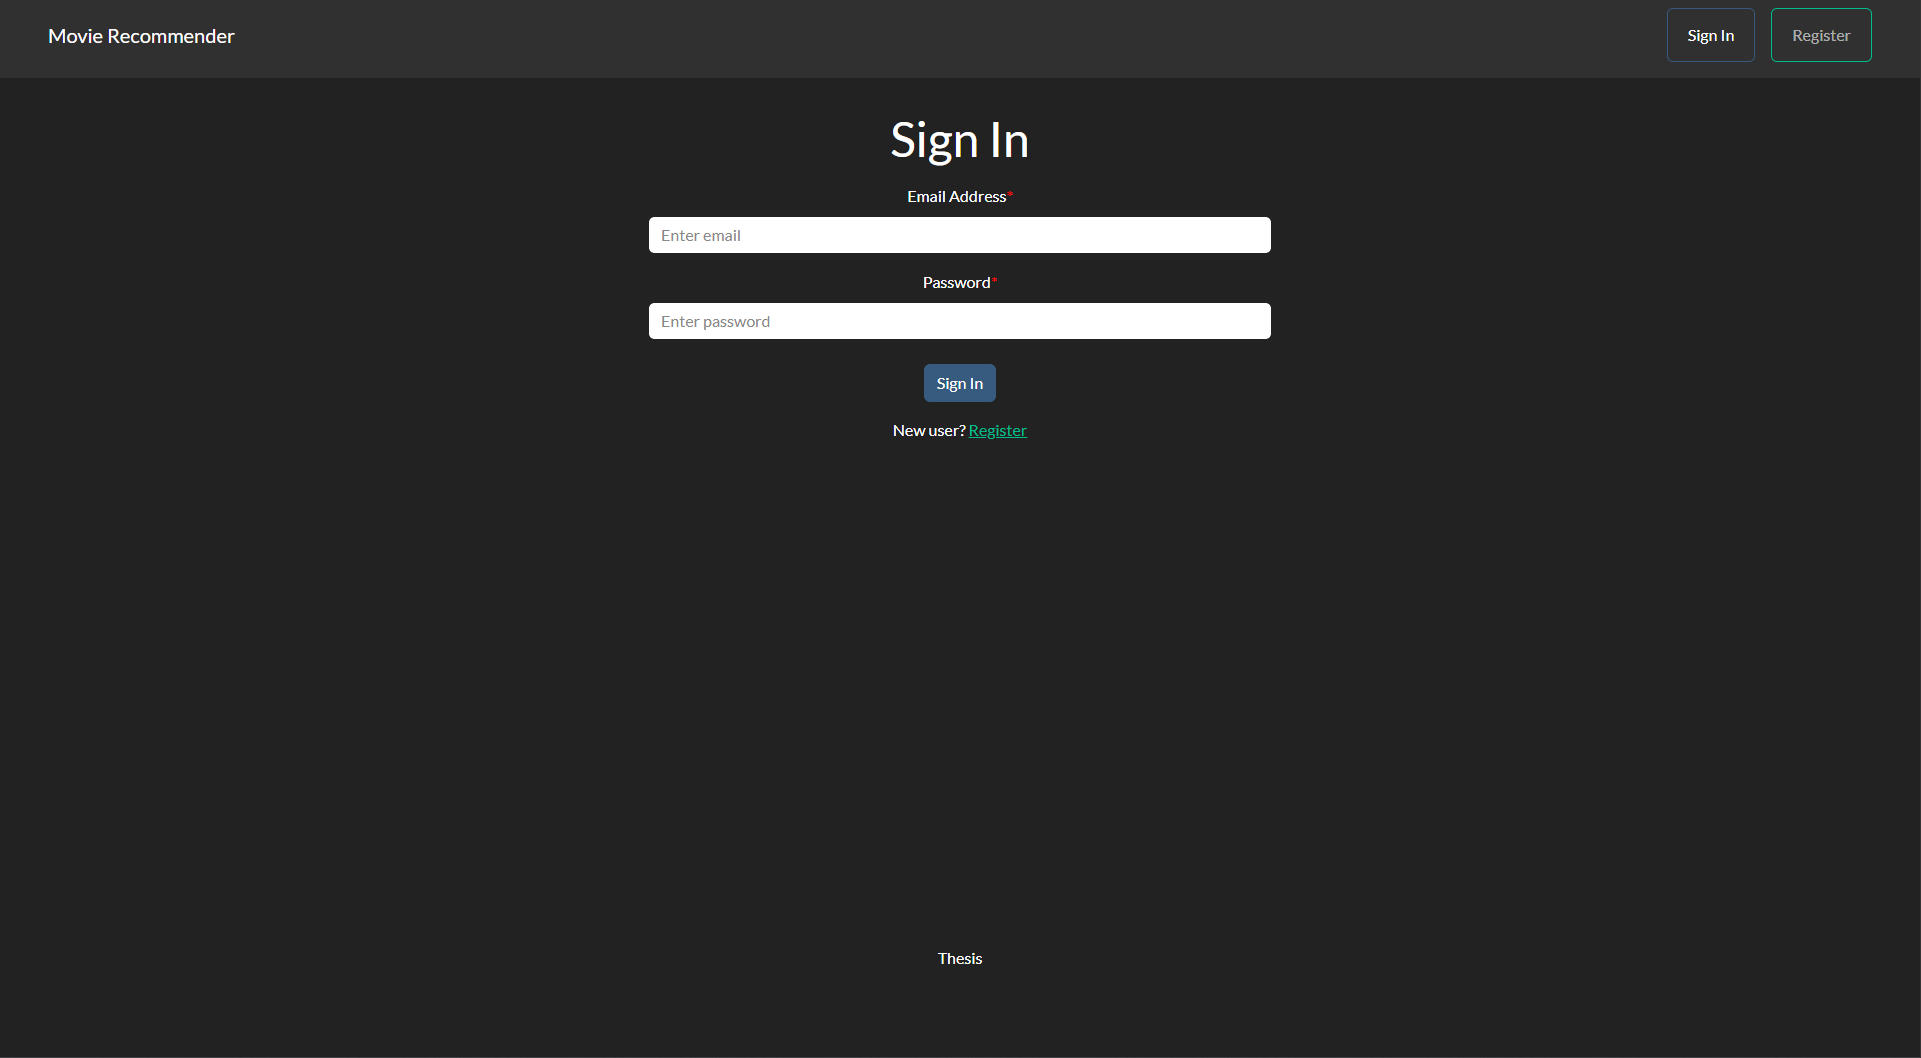
\includegraphics[width=14cm]{images/frontend-login-1.png}
	\caption[Bejelentkezési felület]{Bejelentkezési felület}
	\label{fig-sign-in}
\end{figure}

A két felület és a folyamat nagyon hasonló. Validációt nem implementáltam, az \emph{Email Address} mezőhöz a \emph{HTML input element type} értékét ``email''-re állítottam, valamint a piros csillaggal jelölt mezőknél \emph{required}-ként (kötelezőként) definiáltam az inputokat.

A \emph{Sign In} (bejelentkezés) gomb megnyomását követően az alkalmazás beküldi a \emph{backend szolgáltatás} részére a szükséges adatokat (\ref{fig-sign-in-network}. és \ref{fig-sign-in-payload}. ábrák).

\begin{figure}[H]
	\centering
	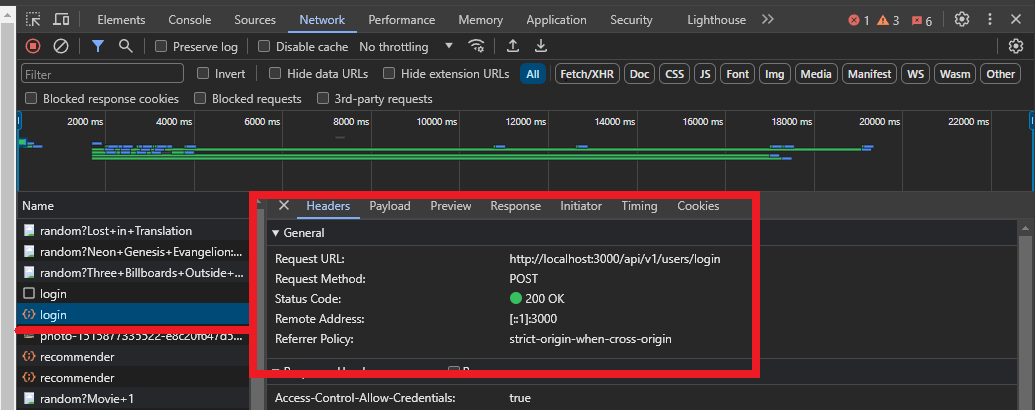
\includegraphics[width=14cm]{images/frontend-login-2.png}
	\caption[Bejelentkezési űrlap beküldése a Backend részére]{Bejelentkezési űrlap beküldése a Backend részére}
	\label{fig-sign-in-network}
\end{figure}

A \emph{backend szolgáltatás} a \emph{./backend-service/src/index.ts} fájlban az \emph{app.use('/api/v1/users', userRouter);} sorral átirányítjuk a kérést az \emph{userRouter}-nek. Majd az \emph{userRouter}-ben definiált \emph{userRouter.post('/login', UserController.loginUser)} sor meghívja az \emph{UserController.loginUser} statikus metódusát, ami látható \aref{code-backend-user-controller-login}. kódban.

\lstinputlisting[style=ts,caption=Backend szolgáltatás - UserController.userLogin\(\),label=code-backend-user-controller-login]{codes/user-controller-login.ts}

\begin{figure}[H]
	\centering
	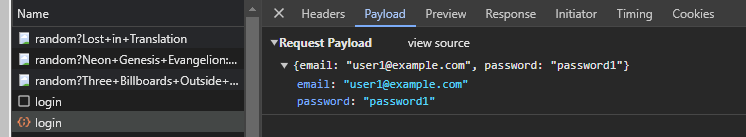
\includegraphics[width=12cm]{images/frontend-login-network-payload.png}
	\caption[Bejelentkezési űrlap tartalma]{Bejelentkezési űrlap tartalma}
	\label{fig-sign-in-payload}
\end{figure}

\Aref{code-backend-user-controller-login}. kód 3. sorában validáljuk a kérésben küldött adatokat, majd a 4. sorban az \emph{UserService}-t használva, az \emph{UserDAO} segítségével megnézzük, hogy létezik-e felhasználó ezzel az \emph{email-jelszó} párossal. Ha a felhasználó megtalálható az adatbázisban és a jelszó is stimmel, válaszként visszaküldjük az adatbázisból származó felhasználó adatokat \emph{JSON formátumban}, hozzá egy \emph{200}-as (OK) HTTP kódot társítva, jelezve, hogy minden rendben ment. Ez látható \aref{fig-sign-in-response}. ábrán is. Ellenkező esetben egy \emph{UnauthorizedError}-t dobunk. 

\begin{figure}[H]
	\centering
	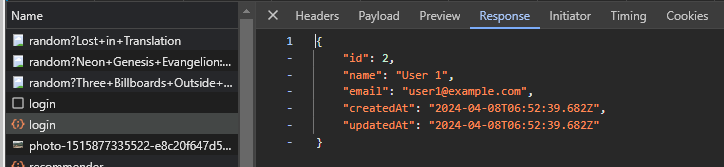
\includegraphics[width=12cm]{images/frontend-login-3.png}
	\caption[Backend HTTP válasza a bejelentkezésre]{Backend HTTP válasza a bejelentkezésre}
	\label{fig-sign-in-response}
\end{figure}

Emellett \aref{code-backend-user-controller-login}. kód 7. sorában látható, hogy meghívunk egy függvényt, melyet \aref{code-backend-setup-jwt-cookie}. kód mutat részletesebben.

\lstinputlisting[style=ts,caption=Backend szolgáltatás - HttpOnly cookie Beállítása,label=code-backend-setup-jwt-cookie]{codes/setup-jwt-cookie.ts}

\Aref{code-backend-setup-jwt-cookie}. kód 8. sorában létrehozunk egy \emph{JWT token}t (lásd \ref{subsec-authentikacio-authorizacio}. fejezet), amit a \emph{protect middleware}-ben (\ref{code-backend-auth-middleware}. kód) fogunk használni. Ezzel fogjuk ellenőrizni, hogy érvényes-e a token, azaz, hogy mi a benne található \emph{userId} és hogy lejárt-e. Ezt a tokent visszaküldjük \emph{HttpOnly cookie}ként a 12-16. sorokban látható módon (a cookie látható \aref{fig-sign-in-cookie}. ábrán) és eltároljuk a \emph{frontenden} melyeket a bejelentkezés után a kliens automatikusan csatolni fog a \emph{HTTP(S)} kérésekhez. Így a \emph{backend} számára a kérésekkel elérhetővé válik a token és tudjuk \emph{autentikálni} a felhasználót, ezáltal \emph{privát útvonalakat} tudunk létrehozni, ahogy az ajánlások útvonala is az.

\begin{figure}[H]
	\centering
	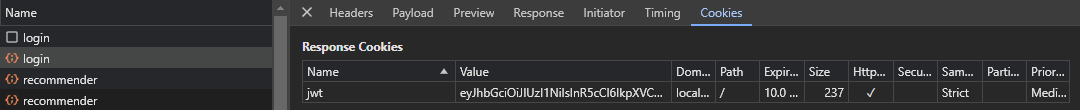
\includegraphics[width=14cm]{images/frontend-login-response-cookie.png}
	\caption[Bejelentkezésnél beállított Cookie]{Bejelentkezésnél beállított Cookie}
	\label{fig-sign-in-cookie}
\end{figure}

Így tehát, ha a bejelentkezést követően le szeretnénk kérni a \emph{backend}től a felhasználónak készített \emph{Top-N} ajánlásokat, a \emph{frontend} ahhoz a kéréshez már automatikusan társítja a kapott cookiet. Mindez \aref{fig-frontend-rec-request-cookies}. ábrán látható. A felső keretben a hívott URL (Request URL), a használt \emph{HTTP metódus} (Request Method) valamint a válasz státusza (Status Code), mely utóbbi 200 OK, azaz sikeres. Alatta a \emph{Request Headers} részben láthatjuk a legalsó keretben lévő \emph{Cookie} mezőt, mely tartalmazza a \emph{backendtől kapott JWT tokent}. Ha hiányzó tokennel vagy cookie-val, azaz bejelentkezés nélkül végeznénk el ugyanezt a hívást, esetleg lejárt vagy invalid a token, akkor \emph{401 Unauthorized} kódot kapnánk.

\begin{figure}[H]
	\centering
	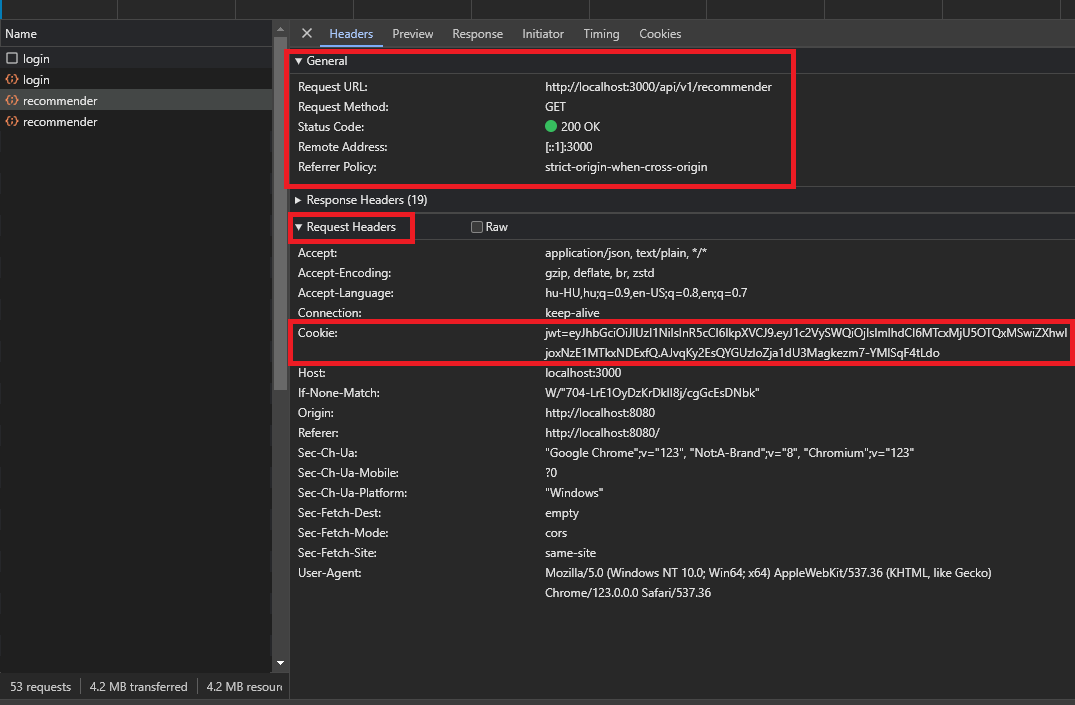
\includegraphics[width=14cm]{images/frontend-recommender-request.png}
	\caption[Ajánlások kérése a backend-service API-tól]{Ajánlások kérése a backend-service API-tól}
	\label{fig-frontend-rec-request-cookies}
\end{figure}

\subsection{Személyre szabott ajánlások}
Végül, de nem utolsó sorban elérkeztünk a pontra, ahol mindez összeáll egy egésszé, és a bejelentkezett felhasználó számára lekérjük a \emph{Top-N} ajánlást.

Ahogy azt \aref{fig-frontend-rec-request-cookies}. ábrán is látható (a bal sávban), bejelentkezést követően egyből le is kérjük a felhasználónak már előre elkészített ajánlásokat (lásd \ref{subsubsec-modell-betanitasa-majd-mentese}. fejezet). Ehhez a \emph{backend szolgáltatás} \emph{recommendations API}-ját hívja meg a frontend, \aref{demo-autentikacio}. fejezetben tárgyalt \emph{cookie}-val ellátva. Ez a \emph{cookie} tartalmaz egy \emph{JWT tokent}, melyet használva a \emph{./backend-service/src/\allowbreak{}middlewares/auth-middleware.ts} fájlban definiált \emph{protect köztes szoftvert} (middleware) -- mely \aref{code-backend-auth-middleware}. kódban látható -- alkalmazva \emph{dekódoljuk} és \emph{validáljuk} az ábra 13. sorában, majd az \emph{UserService}-t és a tokenben tárolt \emph{userId}-t használva lekérjük a felhasználó adatait az adatbázisból, ami a 18. sorban olvasható. A 19. sorban \emph{a felügyeleti lánc elvét} (the chain of responsibility)\footnote{The chain of responsibility-ről bővebben: \url{https://www.geeksforgeeks.org/chain-responsibility-design-pattern/}} használva, a \emph{reqeust} objektumhoz, melyet a \emph{middleware} tovább ad a következő \emph{middleware}-nek, létrehozunk egy \emph{user} nevű tulajdonságot, és ennek értékül adjuk a Service-től kapott\footnote{Az \emph{UserService} az \emph{UserDAO}-t használva szerzi meg az adatbázisban tárolt adatokat.} \emph{user}-t. Végül a 20. sorban hívjuk a következő middleware-t.

\lstinputlisting[style=ts,caption=Backend szolgáltatás - protect middleware,label=code-backend-auth-middleware]{codes/auth-middleware.ts}

Mivel a hívott API végpont el van látva ezzel a köztes szoftverrel, az ezzel a végponttal összekötött \emph{RecommendationController.getTopNRecommendationForLoggedInUser} statikus metódusában elérhető a \emph{reqest} objektum \emph{user} tulajdonsága (property), mely \emph{user\_id} tulajdonságának értékével meghívjuk a  \emph{RecommendationService.getTopNRecom\allowbreak{}mendationsForUserById} (\ref{code-backend-recommender-service-get-top-n}. kód) statikus metódusát és az abból kapott értéket fogjuk visszaküldeni a \emph{frontendnek}.

\lstinputlisting[style=ts,caption=RecommenderService.getTopNRecommendationsForUserById,label=code-backend-recommender-service-get-top-n]{codes/recommender-service-get-top-n.ts}

\Aref{code-backend-recommender-service-get-top-n}. kódban először validáljuk a paraméterként kapott \emph{id}-t majd a felhasználót. Ezután a 8-10. sorokban meghívjuk az \emph{intelligens szolgáltatás} azon végpontját, mely a felhasználó ID-ját használva kikeresi, majd visszaküldi a számára készített ajánlásokat, egy lista formájában, bennük objektumokkal, amik tartalmazzák a \emph{movieID}-t. Ezeket az ID-kat szelektáljuk ki a 11. sorban. Ezt követően a 14. sorban, a \emph{MovieService.getMoviesByArrayOfId}-t hívva megkapjuk a filmek adatait és végül a \emph{backend API} visszaküld egy listát az így kapott filmekről, melyek ``azonnal'' láthatóak a felhasználó számára a \emph{Recommended for you} listában\footnote{A képek csak reprezentációként szolgálnak}, melyet \aref{fig-frontend-for-you}. ábra is mutat.

\begin{figure}[H]
	\centering
	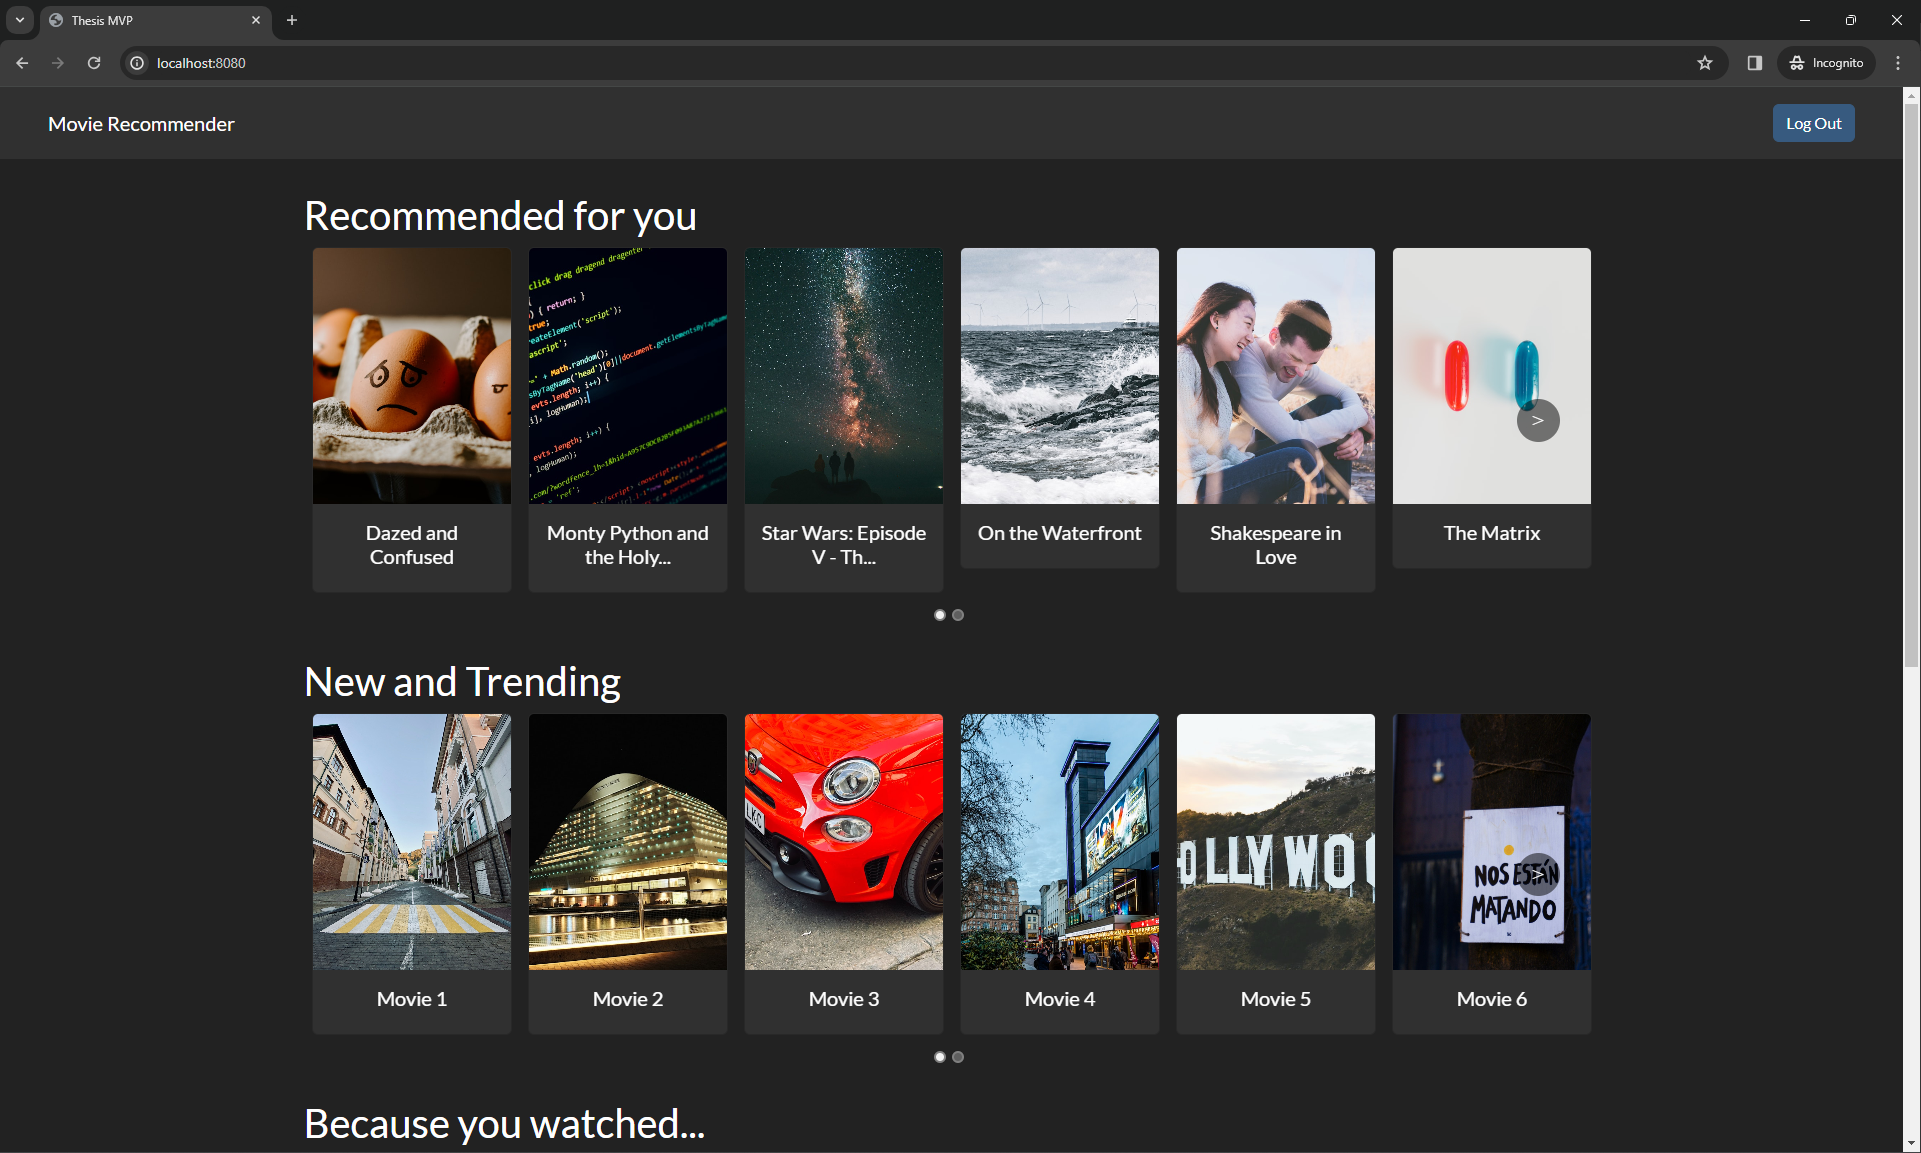
\includegraphics[width=14cm]{images/for-you.png}
	\caption[Személyre szabott ajánlások megjelenítése a böngészőben]{Személyre szabott ajánlások megjelenítése a böngészőben}
	\label{fig-frontend-for-you}
\end{figure}

A \emph{frontenden} ezt az ajánlást az \emph{AppContext}-ből menedzseljük. Az \emph{AppContext}-ből tudunk szolgáltatni funkciókat és állapotokat (state) azoknak a komponensek a számára, melyek \emph{ennek a Context-nek a Provider-jének a gyermekei} (ebben az alkalmazásban gyakorlatilag minden komponens számára).\footnote{React useContext hookjáról bővebben: \url{https://react.dev/reference/react/useContext}} A feladat mérete miatt a \emph{React}-ra jellemző \emph{prop drilling} probléma nincs jelen, azonban az applikáció bizonyos kulcs funkcióit (például autentikáció, ajánlások lekérése) és állapotait (például felhasználó, filmek adatai, hibák) az \emph{AppContext}-tel menedzselem, így központosítva azt. Ezáltal megkapjuk a \emph{HomeScreen} komponens kódját, mely \aref{code-frontend-homescreen}. kódban látható.

\lstinputlisting[style=ts,caption=HomeScreen komponens,label=code-frontend-homescreen]{codes/HomeScreen.ts}

\Aref{code-frontend-homescreen}. kód 8. sorában látható, hogy az \emph{AppContext}-et igénybe vesszük, így hozzáférünk annak \emph{appState} és \emph{getTopN} elemeihez. A 10-14. sorokon lévő \emph{useEffect} minden alkalommal lefut, amikor a 14. sorban lévő függőségek -- \emph{appState.user}, \emph{appState.movies}, \emph{appState.getTopN}, \emph{appState.error} -- megváltoznak. A 11. sorban ellenőrizzük, hogy van-e bejelentkezett felhasználónk (\emph{appState.user}), hogy nincsenek-e még betöltve  filmek\footnote{JavaScriptben az üres tömb (\texttt{[]}) is igaz értéket ad vissza, tehát \texttt{![] === false}} és nincs-e hiba. Ha ezek közül bármelyik hamis, akkor lekérjük a Top-N ajánlási listát a 12. sorban lévő utasítással, mely programkódja \aref{code-frontend-getTopN}. kódban látható.

\lstinputlisting[style=ts,caption=AppContext - getTopN() függvény ,label=code-frontend-getTopN]{codes/getTopN.ts}

Az ajánlásokat a jobb felhasználó élményért \emph{cache}-elem, jelen esetben eltárolom a \emph{local storage}-be. Így amikor meghívom a \emph{getTopN} függvényt, először azt nézem meg, hogy a \emph{local storage}-be vannak-e adatok tárolva (\ref{code-frontend-getTopN}. kód 2-10. sorai), ha vannak, szimplán visszaadom azokat (6. sor), ha nincs, akkor (\emph{axios}-t használva) meghívom a \emph{backend API}-t a 8. sorban látott módon, majd eltárolom a \emph{local storage}-be (9. sor). Ha a folyamat közben hiba lépne fel, azt a 17-18. sorokban látott módon kezeli a program.\footnote{A \emph{handleError} függvényre azért van szükség, mert az \emph{Axios} hibáknak más a felépítésük, így azokat külön kell kezelni. Ebben a funkcióban megvizsgálom, hogy \emph{Axios} dobta-e a hibát, ha igen, akkor azt a \emph{handleAxiosError} függvény fogja a továbbiakban lekezelni.}

\subsubsection{Modell betanítása, majd annak mentése}
\label{subsubsec-modell-betanitasa-majd-mentese}
Azonban ahhoz, hogy az ajánlások bejárják ezt az utat, az \emph{intelligens szolgáltatástól} egészen a \emph{frontendig}, előtte valahogy létre kell őket hozni. \Aref{fig-algoruitmus-metrikak}. ábrán láthattuk, hogy az adatmennyiség és az ajánló algoritmus nagyban befolyásolja, mennyi időt vehet igénybe egy-egy algoritmus betanítása. Valamint lehet, hogy más erőforrásokon más módszerekkel szeretnénk betanítani a modellünket a hatékonyság vagy költségtakarékosság\footnote{Például ha a platform a hívások száma és a futás ideje alapján kalkulálja és számlázza az összeget.} végett. \Aref{fig-mentett-vs-friss}. ábra 2. sorában látható, hogy mennyi időt vesz igénybe egy már betanított modellt és az ahhoz tartozó előre legenerált ajánlásokból létrehozni az összes felhasználó számára egy Top-N ajánlási listát, ahol a $N = 10$.\footnote{\Aref{fig-mentett-vs-friss}. ábrát a \emph{benchmark-loaded-and-fresh-model-svdpp.py} szkripttel hoztam létre.} Ezzel ellenben, a 3. sorban az látható, hogy mennyi időt vesz igénybe, egy új modellt betanítani ugyanazon az adatkészleten és azzal létrehozni ugyanezt a listát. 

A modell és az ajánlások mentéséhez valamint annak betöltésére a \emph{surprise.dump} modulját használtam.

\begin{figure}[H]
	\centering
	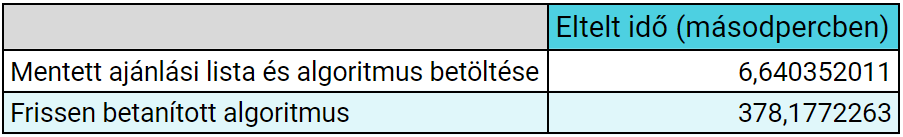
\includegraphics[width=14cm]{images/mentett-vs-friss-algoritmus.png}
	\caption[Kész algoritmus és ajánlások betöltése vs. Frissen betanított algoritmus]{Kész algoritmus és ajánlások betöltése vs. frissen betanított algoritmus\footnotemark}
	\label{fig-mentett-vs-friss}
\end{figure}
\footnotetext{\benchmarkSpecificationSec}


\lstinputlisting[style=python,caption=Intelligens szolgáltatás - \emph{app.py },label=code-flask-app]{codes/app.py}

\Aref{code-flask-app}. kódban látható mindössze 20 sornyi kód létrehoz egy \emph{API}-t a \emph{Flask} csomagot használva. A kód 10. sorában a \emph{load\_dumped.py} fájlban definiált \emph{get\_top\_n} függvényt használva betölti az összes felhasználó számára generált Top-N ajánlási listát (ahol az $N$ a kód 7. sorában van definiálva), ami a \emph{rating\_threshold} (a kód 8. sora) érték fölött van. A kód 12-17. soraiban látható a végpont definiálva, melyet a \emph{backend szolgáltatás} hív. Ez lényegében visszaadja a \emph{top\_n} változóból az útvonal paraméterben kapott, \emph{user\_id} kulcshoz tartozó értéket.\footnote{Ha nincs ilyen kulcs, akkor \emph{None}-t.} Majd ezt a kód 17. sorában visszaküldi \emph{JSON} formátumban. A \emph{backend} ezt továbbítja a \emph{frontend}nek mely megjeleníti azt és a kör bezárul. Ennek a végeredményét láthatjuk \aref{fig-frontend-for-you}. ábrán, valamint mindezt szemlélteti \aref{fig-sequence-diagram-hu}. ábra is.

\begin{figure}[H]
	\centering
	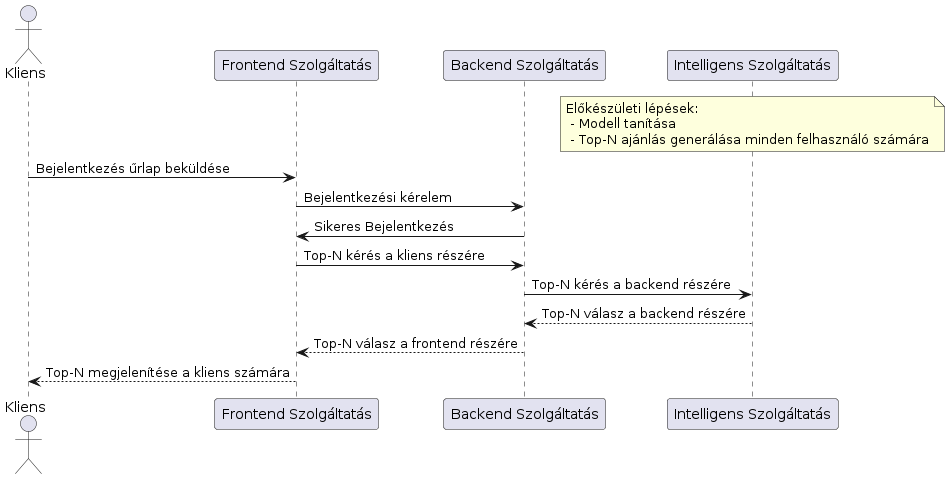
\includegraphics[width=14cm]{images/sequence-diagram-hu.png}
	\caption[Szekvenciadiagram]{Szekvenciadiagram}
	\label{fig-sequence-diagram-hu}
\end{figure}

\chapter*{Összegzés}
\addcontentsline{toc}{chapter}{Összegzés}
Szakdolgozatomban a felhasznált technológiák rövid bemutatása után a gépi tanulás került terítékre. Kifejtettem, mit is takar ez a kifejezés, valamint ismertettem pár felhasználási területét. Ezt követően a gépi tanulás lépéseit taglaltam. Majd az adatról esett szó, azzal kapcsolatos kifejezésekről, feladatokról. Ezután a gépi tanulási típusokat és a hiperparaméter optimalizálást boncolgattam. Később az ajánlórendszereket részleteztem, hogy milyen problémákra nyújtanak megoldást, hogyan lehet őket formálisan leírni, valamint különböző hasonlósági függvényeket is fejtegettem. Majd az ajánlórendszerek eltérő megközelítéseit vettem górcső alá, valamint, hogy hogyan készítjük elő az adatot a tanításra, tesztelésre, és hogyan lehet mérhetővé tenni az ajánlórendszer által generált ajánlások pontosságát, hogyan lehet azok különböző tulajdonságait megvizsgálni. Ezt követően definiáltam az alkalmazásom feladatát, specifikáltam annak rendszertervét, architektúráját. Végül bemutattam a szoftver érdekesebb részeit, hogyan közelítettem meg különböző feladatokat, problémákat, és érdekességképpen prezentáltam pár mérési adatot. Betekintést nyújtottam, onnantól, hogy a felhasználó böngészője először megjeleníti az oldalunkat, az autentikáción át a különböző szolgáltatások kommunikációján keresztül az ajánlások generálásával és azok a megjelenítésével bezárólag.

Úgy érzem, a szakdolgozatomban definiált célt kellőképpen teljesítettem és sikerült egy átfogó képet nyújtanom a gépi tanulásról és ajánlórendszerekről, valamint arról, hogyan lehet mindezt webalkalmazás formájában megvalósítani. A megírásához és az írása alatt egyaránt, magam is rengeteget tanultam és fejlődtem. Remélem aki olvassa hasznát tudja venni ennek az irománynak és ha netán még örömét is leli az olvasásában, annak különösképpen örülök.

\begin{thebibliography}{2}
\addcontentsline{toc}{chapter}{\bibname}

\bibitem{wiki-ts}
TypeScript (2024.02.09.)
\\\url{https://en.wikipedia.org/wiki/TypeScript}

\bibitem{wiki-react}
React (software) (2024.02.09.)
\\\url{https://en.wikipedia.org/wiki/React_(software)}

\bibitem{nodejs-homepage}
Node.js hivatalos oldala
\\\url{https://nodejs.org/en}

\bibitem{expressjs-homepage}
Express.js hivatalos oldala
\\\url{https://expressjs.com/}

\bibitem{chain-of-responsibility}
\textsc{Refactoring Guru}: \emph{Chain of Responsibility} 
\\\url{https://refactoring.guru/design-patterns/chain-of-responsibility}

\bibitem{sequelize}
\textsc{Sequelize} 
\\\url{https://sequelize.org/}

\bibitem{wiki-flask}
Flask (web framework) (2024.02.17.)
\\\url{https://en.wikipedia.org/wiki/Flask_(web_framework)}

\bibitem{surpriselib}
Surprise könyvtár hivatalos oldala
\\\url{https://surpriselib.com/}

\bibitem{surpriselib_docs:prediction_algorithms}
Surprise - prediction\_algorithms package documentation (a \emph{Surprise} könyvtár dokumentációjának egy aloldala) 
\\\url{https://surprise.readthedocs.io/en/stable/prediction_algorithms_package.html}

\bibitem{surpriselib_docs:tune-algorithms-w-gridsearch}
Tune algorithm parameters with GridSearchCV (a \emph{Surprise} könyvtár  dokumentációjának egy aloldala)
\\\url{https://surprise.readthedocs.io/en/stable/getting_started.html#tune-algorithm-parameters-with-gridsearchcv}

\bibitem{wiki-adatbazis}
Adatbázis (2023.09.19.)
\\\url{https://hu.wikipedia.org/wiki/Adatb%C3%A1zis}

\bibitem{postgres-docs}
PostgreSQL dokumentációja
\\\url{https://www.postgresql.org/docs/current/intro-whatis.html}

\bibitem{docker-docs}
Docker dokumentációja
\\\url{https://docs.docker.com/}

\bibitem{docker-overview}
Docker dokumentáció - Docker overview
\\\url{https://docs.docker.com/get-started/overview/}

\bibitem{docker-overview-container}
Docker dokumentáció - What is a container?
\\\url{https://docs.docker.com/guides/docker-concepts/the-basics/what-is-a-container/}

\bibitem{docker-overview-image}
Docker dokumentáció - What is an image?
\\\url{https://docs.docker.com/guides/docker-concepts/the-basics/what-is-an-image/}

\bibitem{docker-compose-docs}
Docker Compose dokumentációja
\\\url{https://docs.docker.com/compose/}

\bibitem{node-docs}
Node.js dokumentációja
\\\url{https://nodejs.org/en/learn/getting-started/introduction-to-nodejs}

\bibitem{wiki-ml}
Machine learning (2024.03.10.)
\\\url{https://en.wikipedia.org/wiki/Machine_learning}

\bibitem{book:ml-for-beginners}
\textsc{Oliver Theobald}: \emph{Machine Learning For Absolute Beginners: A Plain English Introduction (Second Edition)} (2021)

\bibitem{wiki-aihun}
Mesterséges Intelligencia (2024.03.12.)
\\\url{https://hu.wikipedia.org/wiki/Mesters%C3%A9ges_intelligencia}

\bibitem{wiki-aieng}
Artificial Intelligence (2024.03.08.)
\\\url{https://en.wikipedia.org/wiki/Arificial_intelligence}

\bibitem{ml-lifecycle}
The Machine Learning Life Cycle Explained (2020. október)
\\\url{https://www.datacamp.com/blog/machine-learning-lifecycle-explained}

\bibitem{featureengineeringmagyaritas}
Feature engineering magyarul (2012.05.13.)
\\\url{https://angolulblog.wordpress.com/2012/05/13/feature-engineering-magyarul/}

\bibitem{introduction-to-statistical-learning}
\textsc{Gareth James}: \emph{An Introduction to Statistical Learning: with Applications in R}, (2013.)

\bibitem{gepitanulasalapfogalmak}
\textsc{Farkas Richárd}: \emph{Gépi tanulás alapfogalmai}
\\\url{https://www.inf.u-szeged.hu/~rfarkas/ML20/alapfogalmak.html}

\bibitem{bioinformatics-in-ml}
\textsc{Sindhu V., Nivedha S., Prakash M.}: \emph{An Empirical Science Research on Bioinformatics in Machine Learning. (2020. Február)} \textit{Journal of Mechanics of Continua and Mathematical Sciences}
\\\url{https://www.journalimcms.org/special_issue/an-empirical-science-research-on-bioinformatics-in-machine-learning}

\bibitem{tabular-data-def}
What is Tabular Data? (Definition \& Example), (2022.03.25.)
\\\url{https://www.statology.org/tabular-data/}

\bibitem{supervised-learning-google}
Supervised Learning
\\\url{https://cloud.google.com/discover/what-is-supervised-learning#section-5}

\bibitem{gepi-tanulas-3-fo-tipusa}
A gépi tanulás 3 fő típusa
\\\url{https://netliferobotics.hu/blog/a-gepi-tanulas-3-fo-tipusa}

\bibitem{unsupervised-learning-google}
Unsupervised Learning
\\\url{https://cloud.google.com/discover/what-is-unsupervised-learning}

\bibitem{wiki-klaszteranalízis}
Klaszteranalízis (2023.03.15.)
\\\url{https://hu.wikipedia.org/wiki/Klaszteranal%C3%ADzis}

\bibitem{semi-supervised-learning-mit}
\textsc{Olivier Chapelle, Bernhard Schölkopf, Alexander Zien}: \emph{Semi-Supervised Learning}, 2006
\\\url{https://www.molgen.mpg.de/3659531/MITPress--SemiSupervised-Learning.pdf}

\bibitem{mi-a-gepi-tanulas}
Mi a gépi tanulás?
\\\url{https://www.sap.com/hungary/products/artificial-intelligence/what-is-machine-learning.html}

\bibitem{what-is-reinforcement-learning}
What is reinforcement learning?
\\\url{https://aws.amazon.com/what-is/reinforcement-learning}

\bibitem{aws-hyperparameter-tuning}
What is Hyperparameter Tuning?
\\\url{https://aws.amazon.com/what-is/hyperparameter-tuning}

\bibitem{wiki-hyperparameter-optimization}
Hyperparameter optimization, (2024.01.04.)
\\\url{https://en.wikipedia.org/wiki/Hyperparameter_optimization}

\bibitem{wiki-ajánlórendszer-marketing}
Ajánlórendszer (marketing), (2023.04.20.)
\\\url{https://hu.wikipedia.org/wiki/Aj%C3%A1nl%C3%B3rendszer_(marketing)}

\bibitem{wiki-recommender-system}
Recommender system (2024.03.11.)
\\\url{https://en.wikipedia.org/wiki/Recommender_system}

\bibitem{werner-ajanlo-rendszer}
\textsc{Werner Ágnes}: \emph{Ajánló rendszerek}, 2019

\bibitem{wiki-collaborative-filtering}
Collaborative filtering (2024.02.07.)
\\\url{https://en.wikipedia.org/wiki/Collaborative_filtering}

\bibitem{wiki-matrix-factorization}
Matrix factorization (recommender systems), (2023.12.26.)
\\\url{https://en.wikipedia.org/wiki/Matrix_factorization_(recommender_systems)}

\bibitem{hybrid-user-item-based-collaborative-filtering}
\textsc{Nitin Pradeep Kumar, Zhenzhen Fan}: \emph{Hybrid User-Item Based Collaborative Filtering}, 2015. \\\url{https://www.sciencedirect.com/science/article/pii/S1877050915023492}

\bibitem{book:introduction-to-data-minging}
\textsc{Pang-Ning Tan, Michael Steinbach, Vipin Kumar}: \emph{Introduction to Data Mining}, 2014.

\bibitem{journal-neural-collaborative-filtering}
\textsc{Xiangnan He, Lizi Liao, Hanwang Zhang, Liqiang Nie, Xia Hu, Tat-Seng Chua}: \emph{Neural Collaborative Filtering}. 2017 IEEE Conference on Computer Communications (INFOCOM), 2017. 
\\\url{https://arxiv.org/abs/1708.05031}.

\bibitem{recommender-systems-the-textboox}
\textsc{Charu C. Aggarwal}: \emph{Recommender Systems: The Textbook}, 2016.

\bibitem{the-adaptive-web}
\textsc{Peter Busilovsky}: \emph{The Adaptive Web}, 2007.

\bibitem{wiki-hosszu-farok}
Hosszú farok (2024.03.11.)
\\\url{https://hu.wikipedia.org/w/index.php?title=Hossz%C3%BA_farok}

\bibitem{wiki-cosine-similarity}
Cosine similarity (2024.02.15.)
\\\url{https://en.wikipedia.org/wiki/Cosine_similarity}

\bibitem{wiki-skalaris-szorzat}
Skaláris szorzat (2024.02.10.)
\\\url{https://hu.wikipedia.org/wiki/Skal%C3%A1ris_szorzat}

\bibitem{wiki-euklideszi-norma}
Euklideszi norma (2023.07.12.)
\\\url{https://hu.wikipedia.org/wiki/Euklideszi_norma}

\bibitem{wiki-tavolsag}
Távolság (2023.12.25.)
\\\url{https://hu.wikipedia.org/wiki/T%C3%A1vols%C3%A1g}
	
\bibitem{wiki-korrelacios-egyutthato}
Korrelációs együttható (2022.01.09.)
\\\url{https://hu.wikipedia.org/wiki/Korrel%C3%A1ci%C3%B3s_egy%C3%BCtthat%C3%B3}

\bibitem{wiki-tf-idf}
tf-idf (2024.03.17.)
\\\url{https://en.wikipedia.org/wiki/Tf%E2%80%93idf}

\bibitem{journal-netflix-prize-and-svd}
\textsc{Stephen Gower}: \emph{Netflix Prize and SVD}, 2014.04.18.

\bibitem{matrix-factorization-techniques-for-rec-sys}
\textsc{Y. Koren, R. Bell, C. Volinsky}: \emph{Matrix Factorization Techniques for Recommender Systems.} IEE Computer Society, 2009

\bibitem{wiki-latent-and-observable-variables}
Latent and observable variables (2024.01.26.)
\\\url{https://en.wikipedia.org/wiki/Latent_and_observable_variables}

\bibitem{szingularis-ertek-felbontas-es-fuggvenyillesztes}
\textsc{Kormányos Andor}: \emph{Szinguláris érték felbontás és függvényillesztés}, 2020.02.20.

\bibitem{wiki-diagonalis-matrix}
Diagonális mátrix (2023.02.18.)
\\\url{https://hu.wikipedia.org/wiki/Diagon%C3%A1lis_m%C3%A1trix}

\bibitem{overfitting}
Overfitting (2020.11.16.)
\\\url{https://lexiq.hu/overfitting}

\bibitem{szupercella:elorejelzesek-verifikacioja}
Előrejelzések verifikációja II. (2015.04.14.)
\\\url{https://www.szupercella.hu/elorejelzesek_verifikacioja_2}

\bibitem{surpriselib:accuracy-module}
Surprise documentation - Accuracy Module
\\\url{https://surprise.readthedocs.io/en/stable/accuracy.html#surprise.accuracy.rmse}

\bibitem{wiki-hit-rate}
Hit rate (2022.09.29.)
\\\url{https://en.wikipedia.org/wiki/Hit_rate}

\bibitem{article-evaulating-a-real-life-recommender-system}
\textsc{Susan Li}: \emph{Evaluating A Real-Life Recommender System, Error-Based and Ranking-Based}. 2019.01.17.
\\\url{https://towardsdatascience.com/evaluating-a-real-life-recommender-system-error-based-and-ranking-based-84708e3285b}

\bibitem{recommendation-system-evaluation-metrics}
\textsc{Rishabh Bhatia}: \emph{Recommendation System Evaluation Metrics}. 2019.03.18.
\\\url{https://medium.com/@rishabhbhatia315/recommendation-system-evaluation-metrics-3f6739288870}

\bibitem{10-metrics-to-evaluate-rec-and-ranking-systems}
10 metrics to evaluate recommender and ranking systems
\\\url{https://www.evidentlyai.com/ranking-metrics/evaluating-recommender-systems#behavioral-metrics}

\bibitem{linkedin:serendipity}
How can recommender systems learn from serendipitous discoveries and outcomes?
\\\url{https://www.linkedin.com/advice/0/how-can-recommender-systems-learn-from-serendipitous}

\bibitem{evaluation-metrics-for-rec-sys}
\textsc{Claire Longo}: \emph{Evaluation Metrics for Recommender Systems} 2018.11.23.
\\\url{https://towardsdatascience.com/evaluation-metrics-for-recommender-systems-df56c6611093}

\bibitem{recommender-systems-machine-learning-metrics-and-business-metrics}
\textsc{Zuzanna Deutschman}: \emph{Recommender Systems: Machine Learning Metrics and Business Metrics}, 2023.08.07.
\\\url{https://neptune.ai/blog/recommender-systems-metrics}

\bibitem{wiki-a/b-testing}
A/B testing (2024.03.29.)
\\\url{https://en.wikipedia.org/wiki/A/B_testing}

\bibitem{a/b-testing-guide}
A/B Testing Guide
\\\url{https://vwo.com/ab-testing/#how-to-perform-an-a-b-test}

\bibitem{journal-the-definition-of-novelty-in-rec-systems}
\textsc{Liang Zhang}: \emph{The Definition of Novelty in Recommendation System}
\\\url{https://pdfs.semanticscholar.org/e417/a959f8431a61e9cd74e726ea6367f00a82d6.pdf}

\bibitem{wiki-system-design}
Systems Design (2024.02.15.)
\\\url{https://en.wikipedia.org/wiki/Systems_design}

\bibitem{the-complete-guide-to-system-design-in-2024}
The complete guide to System Design in 2024, (2024.02.15.)
\\\url{https://www.educative.io/blog/complete-guide-to-system-design}

\bibitem{wiki-szolgaltatasorientalt-architektura}
Szolgáltatásorientált architektúra (2023.09.15.)
\\\url{https://hu.wikipedia.org/wiki/Szolg%C3%A1ltat%C3%A1sorient%C3%A1lt_architekt%C3%BAra}

\bibitem{mvp-es-mme-jelentese}
Az MVP és MMF jelentése, célja, szerepe (2023.11.27.)
\\\url{https://promanconsulting.hu/mvp-mmf/}

\bibitem{wiki-authentication}
Authentication (2024.03.29.)
\\\url{https://en.wikipedia.org/wiki/Authentication}

\bibitem{wiki-kozbeekelodeses-tamadas}
Közbeékelődéses támadás ( 2023.11.29.)
\\\url{https://hu.wikipedia.org/wiki/K%C3%B6zbe%C3%A9kel%C5%91d%C3%A9ses_t%C3%A1mad%C3%A1s}

\bibitem{prototyping-a-recommender-system-step-by-step-part-2}
\textsc{Kevin Liao}: \emph{Prototyping a Recommender System Step by Step Part 2: Alternating Least Square (ALS) Matrix Factorization in Collaborative Filtering}, 2018.11.17.
\\\url{https://towardsdatascience.com/prototyping-a-recommender-system-step-by-step-part-2-alternating-least-square-als-matrix-4a76c58714a1}

\bibitem{wiki-benchmark}
Benchmark (computing), (2024.02.20.)
\\\url{https://en.wikipedia.org/wiki/Benchmark_(computing)}

\bibitem{wiki-self-information}
Information content (2024.03.21.)
\\\url{https://en.wikipedia.org/wiki/Information_content}

\bibitem{wiki-dip-magyar}
A függőség megfordításának elve (2023.06.16.)
\\\url{https://hu.wikipedia.org/wiki/A_f%C3%BCgg%C5%91s%C3%A9g_megford%C3%ADt%C3%A1s%C3%A1nak_elve}

\bibitem{wiki-dependency-injection-magyar}
A függőség befecskendezése (2023.05.30.)
\\\url{https://hu.wikipedia.org/wiki/A_f%C3%BCgg%C5%91s%C3%A9g_befecskendez%C3%A9se}

\bibitem{wiki-dto-hun}
Adatátviteli objektum (2020.06.06.)
\\\url{https://hu.wikipedia.org/wiki/Adat%C3%A1tviteli_objektum}
\end{thebibliography}

% Aláírt, szkennelt nyilatkozat beillesztése a szakdolgozat végére
\includepdf{nyilatkozat.pdf}
\end{document}